\chapter{Additional techniques, features, measurements} %%%%%%%%%%%%%%%%%%%%%%%%%%%%%%%%%%%%%%%%%%%

\begin{flushright} {\tiny {\color{gray} chapter8.tex}} \end{flushright}

Solving the Stokes equations and the energy equations is one thing. Doing it in 
a geodynamical context requires a lot of additional techniques. 
\newpage %-----------------------------------------------------------------------------------------
\section{Dealing with a free surface (and mesh deformation)}\label{sec:freesurface} \index{general}{Free Surface}


When carrying out global models, typically  mantle convection, the effect of the free surface
is often neglected/negligeable: topography ranges from $\sim$ 10km depth to $\sim$ 10km height, which 
is very small compared to the depth of the mantle ($\sim$ 3000km). 

However, it has long been regognised that there is a feedback between topography and crust/lithosphere
deformation: the surface of the Earth reflects the deeper processes, from orogeny, back-arc basins, 
rifts, mid-ocean ridges, etc ... (see for instance \cite{brau10}).

\begin{remark}
Free surface flows are not unique to Earth sciences, and their modelling has given rise to many studies 
and textbooks. A typical free-surface flow problem in the CFD literature is the so-called 'dam break' 
problem \cite{moeb99,bacp07,liir07,lemx08,homa09,anco09}. Other occurrences involve 
sea waves, flow over structures, flow around ships, mould filling, flow with bubbles \cite{liir07}.
\end{remark}
 
What distinguishes geodynamics free surface modelling from its engineering 
counterpart is (i) the absence of surface tension, (ii) the fact that the fluids under consideration are
Stokesian, (iii) their rheology is complex (the elastic and plastic components can be 
dominant at the surface).

%There are to main modelling approaches employed in Computational Geodynamics: the so-called 
%'sticky air' approach and the Arbitrary-Lagrangian approach.

The problem of dealing with a free surface can be deceptively simple at first glance: as mentioned before the
amplitude of surface movement is often less than 1\% of the domain size. Isostacy-driven movements are
easy to deal with since the movement is vertical (and often characteried by  long wavelength). However, computational 
problems quickly arise in subduction modelling: the downgoing lithosphere subducts below the 
overriding plate and the relative convergence of the two is likely to generate a cusp at the trench. The presence
of shear bands intersecting the surface accentuates the problem:

\begin{center}
\includegraphics[width=13cm]{images/freesurface/matv15} \\
{\tiny Taken from Maffione et al \cite{matv15}. Example of free surface deformation above 
intra-oceanic subduction initiation}
\end{center}

\begin{remark} It is difficult to talk about free surface without including the underlying mesh. What follows
should be read alongside Section~\ref{sec:meshes}.
\end{remark}

%.......................................
\subsubsection{The fully Lagrangian approach}

\index{general}{Bow-tied element}

In this case the mesh is deformed with the velocity (or displacement) computed on its nodes. 
It is sometimes called 'body fitting' \cite{crsg12} or 'boundary fitted'. 
In the case when large deformation occurs (which is rather frequent in geodynamics - 
think about subduction or rifting processes where materials end up moving 100's or 1000's of km, horizontally
and/or vertically), it leads to highly deformed elements, and in some case even bow-tied:

\begin{center}
\frame{\includegraphics[width=4.5cm]{images/freesurface/b00}}
\frame{\includegraphics[width=4.5cm]{images/freesurface/b01}}
\frame{\includegraphics[width=4.5cm]{images/freesurface/b02}}\\
\frame{\includegraphics[width=4.5cm]{images/freesurface/b03}}
\frame{\includegraphics[width=4.5cm]{images/freesurface/b05}}
\frame{\includegraphics[width=4.5cm]{images/freesurface/b07}}\\
\frame{\includegraphics[width=4.5cm]{images/freesurface/b08}}
\frame{\includegraphics[width=4.5cm]{images/freesurface/b09}}
\frame{\includegraphics[width=4.5cm]{images/freesurface/b10}}\\
{\tiny Example of a free surface evolution above a sinking sphere. The isostatic rebound above the sphere 
generates a cusp which, if no special measure is taken, ultimately leads to a bow-tied element. Once this 
occurs the simulation stops since the mapping of the bow-tied element to the reference element yields to
wrong elemental matrix. Curtesy of M. Fraters}
\end{center}

In the mildest cases this does not occur but it has long been established that 
large mesh deformation yields low accuracy calculations, 
especially when angles between edges become small or large. 
One way to overcome this problem is to remesh, i.e. generate a better mesh based on the 
available information on the deformed one. In 2D this is routinely done, especially when 
triangular elements are used. In 3D, multiple remeshing are very costly and it is generally
avoided.  
Note also that re-meshing often involves some form of interpolation and therefore some unwanted 
numerical diffusion. 
When deformation is reasonably small, fully lagrangian methods work and have been used in 
geodynamics \cite{hach96b,mera80,labp00}.

\begin{center}
\includegraphics[width=8cm]{images/freesurface/labp00}\\
{\captionfont Taken from \cite{labp00}. Upper-crustal faulting, note that the bottom and the top surface are deformed.}
\end{center}


\begin{center}
\begin{minipage}{0.45\textwidth}
\centering
\includegraphics[width=7cm]{images/freesurface/guez96}\\
{\captionfont Taken from \cite{guez96}. Subduction model, topographic expression is shown without vertical exaggeration}. 
\end{minipage}\hfill
\begin{minipage}{0.45\textwidth}
\centering
\includegraphics[width=6cm]{images/freesurface/gowo93}\\
{\captionfont Taken from \cite{gowo93}. Asymmetric lithospheric extension.}
\end{minipage}
\end{center}







GET:
Crook et al. 2006, and references therein \cite{crwy06})
Beaumont et al. 1994;  \cite{befh94}


%.......................................
\subsubsection{The Eulerian approach: using sticky air}
\index{general}{Sticky Air}

Sticky air is the default option for numerical methods which mesh 
cannot be deformed (typically the finite difference method).
In this case, the air above the crust/sediments is modelled as a zero-density fluid with 
very low viscosity (see for instance the early article by Zaleski and Julien \cite{zaju92}). 
One problem quickly arises when one realises that the viscosity of the 
air ($\sim 18.5\cdot10^{-6}$ Pa$\cdot$s\footnote{\url{https://en.wikipedia.org/wiki/Viscosity}})
is almost 25-30 orders of magnitude lower than the (effective) viscosity of Earth materials. 
Real air viscosity cannot therefore be used because of 1) round-off errors, 2) extremely 
poorly-conditioned matrices. Low viscosities around $10^{16}-10^{19}$Pa$\cdot$s are then 
commonly used as they are still negligible next to those of the (plastic) crust, and the 
flow of air parallel to Earth materials only generates extremely small shear and normal stress values
(thereby approaching the true nature of a free surface). 
This approach is the one employed in all the papers based on the I2/I3(EL)VIS code (see Appendix~\ref{app:codes})
and has been benchmarked in Crameri et al. \cite{crsg12}.

This approach has a few advantages:
\begin{enumerate}
\item it is simple to implement 
\item it is compatible with all the standard numerical methods (FEM, FDM,FVM)
\item it avoids (potentially complicated) remeshing
\end{enumerate}
and quite a few drawbacks:
\begin{enumerate}
\item it increases the size of the computational domain, thereby adding more unknowns to the linear system: in \cite{scbe08} the air layer is set to 50km while the lithospheric domain underneath is 700km thick;
\item it requires the use of averaging all along the free-surface
where very large viscosity contrasts are present. Here is what Poliakov and Podlachikov \cite{popo92}
say about the sticky air method:
"Zaleski \& Julien \cite{zaju92} used a top layer with a very low
viscosity and density to represent air or water above the
surface. This allows a simple representation of the free
surface. However, due to the very high viscosity and density
contrast and diffusion between the top layer and the
underlying layers, calculations sometimes become unstable
and give significant errors."

\item it can showcase air entrainment:
\begin{center}
\includegraphics[width=8cm]{images/freesurface/scbe08}\\
{\small Taken from \cite{scbe08}. Details of the entrainment and lubrication of the soft surface layer. 
Light blue particles are sticky air particle and are found to greatly alter the viscosity
of the subduction channel.}
\end{center}
\item it is not clear how thick the air layer must be
\item it often requires to ascribe thermal parameters to the air;
\item it makes the implementation of Dirichlet or Neuman boundary conditions for temperature at the surface less
obvious.
\item it makes the coupling with surface processes codes less straightforward.
\item its accuracy depends on the method used to track materials in the rest of the code (markers, level sets, ...). If markers are used, the free surface position is then known up to the average distance between markers.
\item it negatively impacts the condition number of the matrix.
\end{enumerate}

The sticky air approach is employed by various codes in the subduction benchmark study \cite{scbe08}

The term 'sticky water' is sometimes employed too. The dynamic viscosity of water is about 
$10^{-3}$Pa$\cdot$s so that it is also negligible compared to the viscosity of Earth materials
and the same reasonng as air applies. However, in such a case a density of about 1000kg/m$^3$ 
is then assigned to the layer. REF?

In conclusion, as stated in \cite{crsg12}: "the sticky air method is a good way to
simulate a free surface for Eulerian approaches, provided that its
parameters are chosen carefully."


%..........................................................
\subsubsection{The Arbitrary Lagrangian Eulerian (ALE) approach}
\index{general}{Arbitrary Lagrangian Eulerian} \index{general}{ALE}

It is a very widely used approach in FEM-based geodynamics codes but originates in the field of 
CFD \cite{hiac74,hulz81} and is described at length in \cite{sozo01,dohp04,dohu03}.
To put it very simply, the key idea in the ALE formulation is
the introduction of a computational mesh which can move and deform with a velocity 
independent of the velocity carried by the material particles.

\paragraph{The simple approach in \cite{thie11}.}
What follows is written with a 2D Cartesian model in mind ($Q_1\times P_0$ elements are used).
The computational domain is a rectangle of size $L_x \times  L_y$ 
and a nnx $\times$ nny rectangular grid spanning the simulation
domain is generated.
The grid points constituting the top row of the grid define the
discrete free surface of the domain. Once the Eulerian velocity field
has been computed on these, their position is first updated using a
simple Eulerian advection step (see a,b on figure hereunder):
\[
\vec{r}_i'(t+\delta t) = \vec{r}_i(t) + \vec{v}_i \cdot \delta t
\qquad\qquad
i=1,\dots nnx
\]
The other boundaries of the system remain fixed at locations
$x=0$, $x=L_x$ and $y=0$. Even though the Eulerian grid must conform
to the current domain shape, only vertical motion of grid nodes is
allowed. It is therefore necessary to resample the predicted free
surface given by $\vec{r}_i'$ at equidistant positions between $x=0$ and $x=L_x$.
The resampling is carried out either with Spline functions or a 
moving least square algorithm. 
Finally, the vertical position of all the nodes corresponding
to column $i\in [1,nnx]$ is recalculated so that they are equidistant, 
as sketched in Figure d. This has the advantage of keeping
the mesh distortion to a minimum in the case of large
deformation.

\begin{center}
\includegraphics[width=9cm]{images/freesurface/ale2d}\\
 {\small The ALE algorithm of \cite{thie11} in 2D. 
(a) Grid and free surface at a given time $t$; 
(b) advection of the free surface; 
(c) resampling of the free surface at equidistant abscissae; 
(d) vertical adjustment of grid nodes in each column at equidistant ordinates.}
\end{center}

The ALE method is used in the SOPALE, SULEC, FANTOM, ELEFANT, and ASPECT codes to name a few
(see Appendix~\ref{app:codes}).


\paragraph{The not-so-simple but rather elegant approach of ASPECT}

What follows is mostly borrowed from Rose et al \cite{robh17}. Their approach 
has the advantage that it does not presuppose a geometry (Cartesian, Spherical, ...)
nor a number of dimensions. It is also designed to work in parallel and on octree-based
meshes, and with various combinations of boundary conditions.
Note that the authors specify that "for moderate mesh deformation, the mesh stays smooth and well
conditioned, though it breaks down for large deformations".


This approach is obtained by simply imposing the obvious condition 
that no particle (fluid parcel) can cross the free surface (because it is a material surface). 
This can be imposed in a straightforward manner by using a Lagrangian description along this surface. 
However, this condition may be relaxed by imposing only the necessary 
condition: $\vec{\upnu}$ equal to zero along the normal to the boundary 
(ie. $\vec{n}\cdot\vec{\upnu} = 0$, where $\vec{n}$ is the outward unit 
normal to the fluid domain). 
The mesh position, normal to the free surface, is determined from the normal component of 
the particle velocity 
and remeshing can be performed along the tangent; 
see, for instance Huerta and Liu, 1989 \cite{huli88} or Braess and Wriggers, 2000 \cite{brwr00} 

As mentioned above the mesh velocity in normal direction at the free surface (with
unit normal $\vec{n}$) has to be consistent with the velocity of the Stokes
velocity solution $\vec{\upnu}(t)$:
\begin{equation}
\vec{\upnu}_{\text{mesh}}(t)\cdot \vec{n} = \vec{\upnu}(t)\cdot \vec{n} 
\qquad
\text{on}
\quad
\Gamma_F
\end{equation}
In ALE calculations the internal mesh velocity is usually undetermined, 
but one wants to smoothly deform the mesh so as to preserve its regularity, 
avoiding inverted or otherwise poorly conditioned cells. 
The mesh deformation can be calculated in many different ways, icluding algebraic 
(as mentioned in the previous paragraph) and PDE based approaches.
The latter is chosen here. 
The Laplace equation is solved where the unknown is the mesh velocity, i.e. 
one must solve:
\begin{equation}
\Delta \vec{\upnu}_{\text{mesh}} = 0\label{eq:fsaspect1}
\end{equation}
subjected to the following boundary conditions:
\begin{eqnarray}
\vec{\upnu}_{\text{mesh}} &=& \vec{0} \qquad\qquad \text{on } \Gamma_0 \\
\vec{\upnu}_{\text{mesh}} &=& (\vec{\upnu}\cdot\vec{n})\vec{n} \qquad \text{on } \Gamma_F \\
\vec{\upnu}_{\text{mesh}}\cdot \vec{n} &=& 0 \qquad\qquad \text{on } \Gamma_{FS} \label{eq:fsaspect2}
\end{eqnarray}
where $\Gamma_{FS}$ is the part of the boundary with free slip boundary conditions, 
$\Gamma_0$ is the no-slip part and $\Gamma_{FS}$ is the free slip part.

Once the mesh velocity has been obtained for all mesh points, these can be moved with 
said velocity. However, it must be noted that the multiple occurences of the normal vector
in the above equations is not without problem as the normal vectors are not well defined on the
mesh vertices, which is where the mesh velocity is defined.

This yields what the author coin the 'quasi-implicit' scheme 
(we have so far neglected any kind of stabilisation):
\begin{enumerate}
\item Solve the Stokes system;
\item Solve for the surface mesh velocity using Equation~\ref{eq:fsaspect3};
\item Solve for the internal mesh velocity using Equations~\ref{eq:fsaspect1}, \ref{eq:fsaspect2}; 
\item Advect the mesh forward in time using displacements determined by
the forward Euler scheme: $\vec{x}(t^{n+1} ) = \vec{x}(t^n ) + \vec{\upnu}_{\text{mesh}} \delta t$.
\end{enumerate}

Note that Rose et al (2017) \cite{robh17} go further than this, propose a 'nonstandard finite difference scheme' 
and make a link with the stabilisation presented in Kaus et al (2010) \cite{kamm10}.

The authors list two simple methods of computing the normals:
\begin{itemize}
\item one can take $\vec{n}$ as the direction of the local vertical,
\item one could compute $\vec{n}$ as some weighted average of the cell normals adjacent to a given
vertex
\end{itemize}
but conclude that they have found that these schemes do not necessarily
have good mass conservation properties.

A better approach is proposed in the form of an $L_2$ projection of the 
normal velocity $\vec{v}\cdot\vec{n}$ onto the free surface $\Gamma_F$. 
Multiplying the boundary conditions 
\[
\vec{\upnu}_{\text{mesh}} = (\vec{\upnu}\cdot\vec{n})\vec{n} 
\]
by a test function $\vec{w}$ and integrating over the free surface part of the boundary, we find:
\begin{equation}
\int_{\Gamma_F} \vec{w}\cdot\vec{\upnu}_{\text{mesh}} d\Gamma 
=
\int_{\Gamma_F} \vec{w}\cdot (\vec{\upnu}\cdot\vec{n})\vec{n} d\Gamma
=
\int_{\Gamma_F} (\vec{w}\cdot\vec{n}) (\vec{\upnu}\cdot\vec{n}) d\Gamma \label{eq:fsaspect3}
\end{equation}
When discretized, this forms a linear system which can be solved for the mesh velocity 
$\vec{\upnu}_{\text{mesh}}$ at the free surface. 
This system, being nonzero over only the free surface, is relatively computationally inexpensive to solve.
The authors unfortunately fail to mention that this approach is particularly 
interesting since the numerical quadrature used to compute the above integrals
require the normal $\vec{n}$ between the nodes and these normals are well defined over each 
segment joining two nodes!\footnote{what if $Q_k$ with $k>1$ elements are used and nodes on the surface
no more form a line? }

In what follows I present in some detail how to carry out the $L_2$ projection to arrive at the surface velocity
for both $Q_1$ and $Q_2$ elements.

I start from the following integral over a $Q_1$ element:
\begin{eqnarray}
\int_{\Gamma_e} N_i \vec{\upnu}_{mesh} d\Gamma
&=& \int N_i \left( \begin{array}{c} u_{mesh} \\ v_{mesh} \end{array} \right) d\Gamma \\
&=& \int N_i 
\left( \begin{array}{cccc}  N_1 & 0 & N_2 & 0 \\ 0 & N_1 & 0 & N_2  \end{array}\right)\cdot
\left( \begin{array}{c} u_1 \\ v_1 \\ u_2 \\ v_2 \end{array} \right) d\Gamma \\
\end{eqnarray}
Writing this equation alternatively for $N_i=N_1,N_2$ yields:
\[
\int_{\Gamma_e} 
\left( \begin{array}{cccc}  
N_1N_1 & 0 & N_1N_2 & 0 \\ 
0 & N_1N_1 & 0 & N_1N_2 \\
N_2N_1 & 0 & N_2N_2 & 0 \\ 
0 & N_2N_1 & 0 & N_2N_2 
\end{array}\right)
\cdot \left( \begin{array}{c} u_1 \\ v_1 \\ u_2 \\ v_2 \end{array} \right) 
d\Gamma 
=
\int_{\Gamma_e} 
\left( \begin{array}{cccc}  
N_1N_1 & 0 & N_1N_2 & 0 \\ 
0 & N_1N_1 & 0 & N_1N_2 \\
N_2N_1 & 0 & N_2N_2 & 0 \\ 
0 & N_2N_1 & 0 & N_2N_2 
\end{array}\right)
d\Gamma \quad 
\cdot \left( \begin{array}{c} u_1 \\ v_1 \\ u_2 \\ v_2 \end{array} \right) 
\]
Turning now to the right hand side %(I denote by $\vec{n}_e$ the normal to the element edge):
$\int_{\Gamma_e} N_i   (\vec{\upnu}\cdot\vec{n}_e)\vec{n}_e  d\Gamma$, it yields the following rhs:
\[
\int_{\Gamma_e}   (\vec{\upnu}\cdot\vec{n}_e)
\left(\begin{array}{c}
N_1 n_x \\ N_1 n_y \\ N_2 n_x \\ N_2 n_y
\end{array}\right)
 d\Gamma
\]
The elemental matrix and rhs must be built for each element and assembled in a 
global matrix and rhs. The solution is the mesh velocity vector at all surface nodes.
the same approach can be taken for $Q_2$ elements:
\begin{eqnarray}
\int_{\Gamma_e} N_i \vec{\upnu}_{mesh} d\Gamma
&=& \int N_i \left( \begin{array}{c} u_{mesh} \\ v_{mesh} \end{array} \right) d\Gamma \\
&=& \int N_i 
\left( \begin{array}{cccccc}  
N_1 & 0 & N_2 & 0 & N_3 & 0\\ 
0 & N_1 & 0 & N_2 & 0 & N_3 
\end{array}\right)\cdot
\left( \begin{array}{c} u_1 \\ v_1 \\ u_2 \\ v_2 \\ u_3 \\ v_3 \end{array} \right) d\Gamma 
\end{eqnarray}
Writing this equation alternatively for $N_i=N_1,N_2,N_3$ yields:
\begin{eqnarray}
&&\int_{\Gamma_e} 
\left( \begin{array}{cccccc}  
N_1N_1 & 0 & N_1N_2 & 0 & N_1N_3 & 0 \\ 
0 & N_1N_1 & 0 & N_1N_2 & 0 & N_1N_3 \\
N_2N_1 & 0 & N_2N_2 & 0 & N_2N_3 & 0 \\ 
0 & N_2N_1 & 0 & N_2N_2 & 0 & N_2N_3 \\
N_3N_1 & 0 & N_3N_2 & 0 & N_3N_3 & 0 \\ 
0 & N_3N_1 & 0 & N_3N_2 & 0 & N_3N_3 \\
\end{array}\right)
\cdot \left( \begin{array}{c} u_1 \\ v_1 \\ u_2 \\ v_2 \\ u_3 \\ v_3 \end{array} \right) 
d\Gamma \nn\\ 
&=&
\int_{\Gamma_e} 
\left( \begin{array}{cccccc}  
N_1N_1 & 0 & N_1N_2 & 0 & N_1N_3 & 0 \\ 
0 & N_1N_1 & 0 & N_1N_2 & 0 & N_1N_3 \\
N_2N_1 & 0 & N_2N_2 & 0 & N_2N_3 & 0 \\ 
0 & N_2N_1 & 0 & N_2N_2 & 0 & N_2N_3 \\
N_3N_1 & 0 & N_3N_2 & 0 & N_3N_3 & 0 \\ 
0 & N_3N_1 & 0 & N_3N_2 & 0 & N_3N_3 
\end{array}\right)
d\Gamma \quad 
\cdot \left( \begin{array}{c} u_1 \\ v_1 \\ u_2 \\ v_2 \\ u_3 \\ v_3 \end{array} \right) 
\end{eqnarray}

The right hand side is then  
\[
\int_{\Gamma_e}   (\vec{\upnu}\cdot\vec{n}_e)
\left(\begin{array}{c}
N_1 n_x \\ N_1 n_y \\ 
N_2 n_x \\ N_2 n_y \\
N_3 n_x \\ N_3 n_y 
\end{array}\right)
 d\Gamma
\]
Having obtained the boundary condition velocity for the Laplace equation, we can now turn our attention 
to solving this ODE. 


Note that Rose et al (2017) \cite{robh17} go further than this and propose a 'nonstandard finite difference scheme' and make a link with the stabilisation presented in Kaus et al (2010) \cite{kamm10}.

In what follows I omit the subscript 'mesh' and focus on the 2D case. The components of the (mesh) velocity
are given by
\[
u^h = \sum_{i=1}^{m_\upnu} N_i^\upnu u_i
\qquad
\qquad
v^h = \sum_{i=1}^{m_\upnu} N_i^\upnu v_i
\qquad
\qquad
\vec{\upnu}^h=\left( 
\begin{array}{c}
u^h \\
v^h 
\end{array}  \right)
\]
We start from the ODE to solve in its strong form:
\[
\Delta \vec{\upnu}^h = \vec{0}
\]
We multiply it by a velocity test function $N_i^\upnu$ and integrate over an element: 
\begin{eqnarray}
&&\vec 0 \nonumber\\
&=& \int_{\Omega_e} N_i^\upnu  \Delta \vec{\upnu}^h \nonumber\\ 
&=&\int_{\Omega_e} N_i^\upnu \Delta \vec\upnu^h dV \nonumber\\
&=&\int_{\Omega_e}  \left(\begin{array}{c}
N_i^\upnu \Delta u^h \\
N_i^\upnu \Delta v^h 
\end{array}\right) dV \nonumber\\
&=&\int_{\Omega_e}  \left(\begin{array}{c}
N_i^\upnu \vec\nabla \cdot \vec\nabla u^h \\
N_i^\upnu \vec\nabla \cdot \vec\nabla v^h 
\end{array}\right) dV \nonumber\\
&=&
\int_{\Omega_e}   \left(\begin{array}{c}
\vec\nabla N_i^\upnu \cdot \vec\nabla u^h \\
\vec\nabla N_i^\upnu \cdot \vec\nabla v^h 
\end{array}\right) dV \nonumber\\
&=&
\int_{\Omega_e}
\left(\begin{array}{c}
\partial_x N_i^\upnu \partial_x u^h + \partial_y N_i^\upnu \partial_y u^h \\ 
\partial_x N_i^\upnu \partial_x v^h + \partial_y N_i^\upnu \partial_y v^h 
\end{array}\right) dV \nonumber\\
&=&\int_{\Omega_e}
\left(
\begin{array}{cccc}
\partial_x N_i^\upnu & \partial_y N_i^\upnu & 0 & 0 \\ 
0 & 0 & \partial_x N_i^\upnu & \partial_y N_i^\upnu  \\ 
\end{array}
\right)
\!\cdot\!
\left(
\begin{array}{c}
\partial_x u^h \\
\partial_y u^h \\
\partial_x v^h \\
\partial_y v^h 
\end{array}
\right) dV \nonumber\\
&=&\int_{\Omega_e}
\left(
\begin{array}{cccc}
\frac{\partial N_i^\upnu}{\partial x} & \frac{\partial N_i^\upnu}{\partial y} & 0 & 0 \\ 
0 & 0 & \frac{\partial N_i^\upnu}{\partial x} & \frac{\partial N_i^\upnu}{\partial y}  \\ 
\end{array}
\right)
\!\cdot\!
\left(
\begin{array}{cccccccccc}
\frac{\partial N_1^\upnu}{\partial x} & 0  & \frac{\partial N_2^\upnu}{\partial x} & 0  & \cdots & \frac{\partial N^\upnu_{m_\upnu}}{\partial x} & 0 \\ \\
\frac{\partial N_1^\upnu}{\partial y} & 0  & \frac{\partial N_2^\upnu}{\partial y} & 0  & \cdots & \frac{\partial N^\upnu_{m_\upnu}}{\partial y} & 0 \\ \\
0 & \frac{\partial N_1^\upnu}{\partial x}  & 0& \frac{\partial N_2^\upnu}{\partial x}  & \cdots & 0 & \frac{\partial N^\upnu_{m_\upnu}}{\partial x}  \\ \\
0 & \frac{\partial N_1^\upnu}{\partial y}  & 0& \frac{\partial N_2^\upnu}{\partial y}  & \cdots & 0 & \frac{\partial N^\upnu_{m_\upnu}}{\partial y}  
\end{array}
\right) 
\!\cdot\!
\left(
\begin{array}{c}
u_1 \\ v_1 \\ u_2 \\ v_2 \\ \dots \\ u_{m_v} \\ v_{m_v} 
\end{array}
\right) dV \nonumber
\end{eqnarray}
Writing this equation for $i=1,...m_\upnu$, we obtain:
\[
\int
\left(
\begin{array}{cccc}
\frac{\partial N_1^\upnu}{\partial x} & \frac{\partial N_1^\upnu}{\partial y} & 0 & 0 \\ 
0 & 0 & \frac{\partial N_1^\upnu}{\partial x} & \frac{\partial N_1^\upnu}{\partial y}  \\ 
\frac{\partial N_2^\upnu}{\partial x} & \frac{\partial N_2^\upnu}{\partial y} & 0 & 0 \\ 
0 & 0 & \frac{\partial N_2^\upnu}{\partial x} & \frac{\partial N_2^\upnu}{\partial y}  \\ 
\vdots & \vdots & \vdots & \vdots \\
\vdots & \vdots & \vdots & \vdots \\
\frac{\partial N_{m_\upnu}^\upnu}{\partial x} & \frac{\partial N_{m_\upnu}^\upnu}{\partial y } & 0 & 0 \\ 
0 & 0 & \frac{\partial N_{m_\upnu}^\upnu}{\partial x} & \frac{\partial N_{m_\upnu}^\upnu}{\partial y}  \\ 
\end{array}
\right)
\cdot
\left(
\begin{array}{cccccccccc}
\frac{\partial N_1^\upnu}{\partial x} & 0  & \frac{\partial N_2^\upnu}{\partial x} & 0  & \cdots & \frac{\partial N^\upnu_{m_\upnu}}{\partial x} & 0 \\ \\
\frac{\partial N_1^\upnu}{\partial y} & 0  & \frac{\partial N_2^\upnu}{\partial y} & 0  & \cdots & \frac{\partial N^\upnu_{m_\upnu}}{\partial y} & 0 \\ \\
0 & \frac{\partial N_1^\upnu}{\partial x}  & 0& \frac{\partial N_2^\upnu}{\partial x}  & \cdots & 0 & \frac{\partial N^\upnu_{m_\upnu}}{\partial x}  \\ \\
0 & \frac{\partial N_1^\upnu}{\partial y}  & 0& \frac{\partial N_2^\upnu}{\partial y}  & \cdots & 0 & \frac{\partial N^\upnu_{m_\upnu}}{\partial y}  
\end{array}
\right) 
\cdot
\underbrace{
\left(
\begin{array}{c}
u_1 \\ v_1 \\ u_2 \\ v_2 \\ \dots \\ u_{m_v} \\ v_{m_v} 
\end{array}
\right) }_{\vec V}
dV
=\vec{0}
\]
or, 
\[
\left( \int_{\Omega_e} {\bm B}^T  \cdot {\bm B} \; dV \right)\cdot \vec{V} = \vec{0}
\]
where ${\bm B}$ is a $(ndim*ndim) \times (m_v*ndofV)$ matrix. This is implemented in Stone 54 \ref{f54}.

\begin{remark}
The integration by parts should have a minus appear but since the left hand side 
is 0, it is not taken into account. 
\end{remark}

\todo[inline]{surface terms arising from the integration by parts are neglected. EXPLAIN WHY!}


\paragraph{Yet another approach \cite{dohp04}}
The unknown position of free surfaces can be computed using the following approach:
for the simple case of a single-valued function $h=h(x,y,t)$, a hyperbolic equation must be solved,
\begin{equation}
\frac{\partial h}{\partial t} + (\vec{ \upnu}\cdot \vec{ \nabla}) h = 0    \label{eqfs1}
\end{equation}
This is the kinematic equation of the surface and has been used, for instance, 
by Ramaswamy and Kawahara (1987), Huerta and Liu, 1988b, 1990; Souli and Zolesio (2001).





\underline{Idea:} Eq. (\ref{eqfs1}) is a simple advection equation. 
One could also add a diffusion operator with a diffusion coefficient $D$.
Low values of $D$ could be used to stabilise the surface while 
higher values (possibly nonlinear ones) could be used to account for simple 
surface processes. 

\begin{equation}
\frac{\partial h}{\partial t} + (\vec{\upnu}\cdot\vec{ \nabla}) h = D \Delta h  \label{eqfs2}
\end{equation}

Also, Hansen and Nielsen \cite{hanl00,hani03} write:
During the entire model evolution surface processes act to re-distribute sediments. 
These processes are modelled by a diffusion equation with a source term enabling the transport 
of sediments to and from the model profile. The transport equation is written
\[
\dot{h}=\nabla\cdot (\kappa \nabla h) + \dot{s}(w)
\]
where $\kappa=200 km^2/Ma$ is the diffusivity of topography and $\dot{s}(w)$ 
is a linear function of water depth. 



The following pictures are taken from Naliboff et al \cite{nabp17} on the topic 
of how complex fault interaction controls continental rifting. It is a beautiful
example (among many) of the importance of free surface geodynamical expression
and large deformation:

\begin{center}
\includegraphics[width=9cm]{images/freesurface/nabp17a}\\
\includegraphics[width=9cm]{images/freesurface/nabp17b}\\
\includegraphics[width=14cm]{images/freesurface/nabp17c}\\
{\captionfont Taken from \cite{nabp17}}
\end{center}

%-------------------------------------------------------
\subsubsection{On the topic of moving internal nodes}

Braess \& Wriggers \cite{brwr00} propose the following interesting algorithm:
"A measure of the quality of a triangular mesh is the quotient of the
outer radius $r_{out}$ and the inner radius $r_{in}$ 
of each element. This quotient is important because it plays a
certain role in a priori error estimates. If an element degenerates this quotient will approach infinity.
Another important feature of good mesh is that no element becomes very large. With these considerations
in mind the penalty function $W$ is defined:
\begin{equation}
W = \sum_{elts} \left( \frac{r_{out}}{r_{in}} \right)^m \left( \frac{r_{out}}{r_0} \right)^n
\end{equation}
where $m$, $n$ and $r_0$ are positive constants. 
For our calculations we chose $m=3$, $n=1$ and $r_0=1$, but the results seem
to depend only slightly on this choice. Whenever a triangle is distorted or very large, this function becomes
very large. A similar penalty function was presented in \cite{jole97} for 
four-node elements. In that case the angles
of the elements are used to construct the penalty function.
In order to regularize a distorted mesh the coordinates of the internal nodes will be chosen such that $W$ is
minimized. It is not necessary to reach the global minimum, a rough approximation is sufficient.
Therefore the minimization of the potential can be done efficiently with standard procedures and will not be
discussed in any detail. This algorithm can also be applied to $h$-adaptive mesh-generation by choosing
appropriate constants $r_0$ for each triangle."\footnote{Indeed, if $r_0$ is the same for all elements
this parameter will not play any role at all in the minimisation process.} 



\vspace{4cm}
This is still WORK IN PROGRESS. I Need to look at those papers:
\cite{raka87}
\cite{huli88}\cite{pobe98}
\cite{bens89}
\cite{sucy00}
\cite{rama90}
\cite{tebm92}(moving pulse)
\cite{dumg11}
\cite{dumy16} 
\cite{anmp15}
\cite{krwd12}
\cite{stcl10}
\cite{maie12}
\cite{guez96}\cite{zhgm96}
\cite{elsp04}
\cite{brwr00}
\cite{pada83}
and talk about free surface stabilisation \cite{kamm10,qube11,dumg11,robh17}.



 
\newpage %-----------------------------------------------------------------------------------------
\section{Picard and Newton \label{ss_nonlinear}} \index{nonlinear} \index{Picard iterations} \index{relaxation}

\todo[inline]{explain why our eqs are nonlinear}

%--------------------------------
\subsubsection{Picard iterations}

Let us consider the following system of nonlinear algebraic equations:
\[
\mathbb{A}(\vec X) \cdot \vec X = \vec b(\vec X)
\]
Both matrix and right hand side depend on the solution vector $\vec X$.

For many mildly nonlinear problems, a simple successive substitution 
iteration scheme (also called Picard method) will converge to the solution
and it is given by the simple relationship:
\[
\mathbb{A}(\vec X^n) \cdot \vec X^{n+1} = \vec b(\vec X^n)
\]
where $n$ is the iteration number. 
It is easy to implement:
\begin{enumerate}
\item guess $\vec X^0$ or use the solution from previous time step
\item compute $\mathbb{A}$ and $\vec b$ with current solution vector $\vec X^{old}$
\item solve system, obtain $T^{new}$
\item check for convergence (are $\vec X^{old}$ and$\vec X^{new}$ close enough?)
\item $\vec X^{old} \leftarrow \vec X^{new}$
\item go back to 2.
\end{enumerate}

There are various ways to test whether iterations have converged. The simplest
one is to look at $\norm{\vec X^{old}-\vec X^{new} }$ (in the $L_1$, $L_2$ or maximum norm)
and assess whether this term is smaller than a given tolerance $\epsilon$. 
However this approach poses a problem: in geodynamics, if two consecutively obtained 
temperatures do not change by more than a thousandth of a Kelvin (say $\epsilon=10^{-3}$K )
we could consider that iterations have converged but looking now at velocities which 
are of the order of a cm/year (i.e. $\sim 3\cdot 10^{-11}$m/s) we would need a tolerance 
probably less than $10^{-13}$m/s. We see that using absolute values for a convergence 
criterion is a potentially dangerous affair, which is why one uses a relative 
formulation (thereby making $\epsilon$ a dimensionless parameter):
\[
\frac{\norm{\vec X^{old}-\vec X^{new}}}{\norm{\vec X^{new}}} < \epsilon
\]
Another convergence criterion is proposed by Reddy (section 3.7.2) \cite{reddybook2}:
\[
\left(
\frac{ (\vec X^{old}-\vec X^{new})\cdot(\vec X^{old}-\vec X^{new} ) }{ X^{new}\cdot X^{new}  } 
\right)^{1/2} < \epsilon
\]
Yet another convergence criterion is used in \cite{thie11}: the means $<\vec X^{old}>$, $<\vec X^{new}>$
as well as the variances $\sigma^{old}$ amd $\sigma^{new}$ are computed, followed by the 
correlation factor $R$:
\[
R= \frac{ <  (\vec X^{old}-<\vec X^{old}>)\cdot( \vec X^{new}-<\vec X^{new}> )>  }{\sqrt{\sigma^{old}\sigma^{new}}}
\]
Since the correlation is normalised, it takes values between 0
(very dissimilar velocity fields) and 1 (very similar fields). The
following convergence criterion is then used: $1-R < \epsilon$.

\todo[inline]{write about nonlinear residual}


Note that in some instances and improvement in convergence rate can be obtained by use of a 
relaxation formula where one first solves
\[
\mathbb{A}(\vec X^n) \cdot \vec X^{\star} = \vec b(\vec X^n)
\]
and then update $\vec X^n$ as follows:
\[
\vec X^n = \gamma \vec X^n + (1-\gamma) \vec X^\star 
\quad\quad\quad
0 < \gamma \leq 1
\]
When $\gamma=1$ we recover the standard Picard iterations formula above.

%------------------------------------------
\subsection{Defect correction formulation}

Work in progress. 

We start from the system to solve:
\[
{\bm A}(\vec X) \cdot \vec X = \vec b(\vec X)
\]
with the associated residual vector $\vec F$ 
\[
\vec F(\vec X) = {\bm A}(\vec X) \cdot \vec X - \vec b(\vec X)
\]
The Newton-Raphson algorithm consists of two steps:
\begin{enumerate}
\item solve $\bm J_k \cdot \delta \vec X_k = -\vec F(\vec X_k)$, or in the 
case of the incompressible Stokes equation FEM system:
\[
\left(
\begin{array}{cc}
\bm J^{{\cal V}{\cal V}}_k & \bm J^{{\cal V}{\cal P}}_k \\
\bm J^{{\cal P}{\cal V}}_k & 0
\end{array}
\right)
\cdot
\left(
\begin{array}{c}
\delta \vec {\cal V}_k \\ \delta \vec {\cal P}_k
\end{array}
\right)
=
\left(
\begin{array}{c}
- \vec F_k^{\cal V} \\ -\vec F_k^{\cal P}
\end{array}
\right)
\]

\item update $\vec X_{k+1} = \vec X_k + \alpha_k \delta \vec X_k$
\end{enumerate}
The defect correction Picard approach consists of neglecting the derivative terms present 
in the $J$ terms (Eqs. 16,17,18 of \cite{frbt19}) so that 
\[
\bm J^{{\cal V}{\cal V}}_k \simeq \K_k 
\quad\quad
\bm J^{{\cal V}{\cal P}}_k \simeq \G 
\quad\quad
\bm J^{{\cal P}{\cal V}}_k \simeq \G^T
\]
and step 1 of the above iterations become:
\[
\left(
\begin{array}{cc}
\K_k & \G \\ \G^T & 0
\end{array}
\right)
\cdot
\left(
\begin{array}{c}
\delta \vec {\cal V}_k \\ \delta \vec {\cal P}_k
\end{array}
\right)
=
\left(
\begin{array}{c}
- \vec F_k^{\cal V} \\ -\vec F_k^{\cal P}
\end{array}
\right)
\]



 %----------------------------
\newpage %-----------------------------------------------------------------------------------------
\section{Convergence criterion for nonlinear iterations\label{sec:nlconvcrit}}\begin{flushright} {\tiny {\color{gray} nlconvcrit.tex}} \end{flushright}

Disclaimer: the topic of nonlinear PDEs solving is vast and has received 
much attention from the mathematical community. In what follows I present 
a few key ideas which are at the core of many codes and publications in 
computational geodynamics.

Looking at the conservation equations that we must solve, i.e. 
conservation of mass, momentum and energy, we find that more often 
than not the coefficients of these PDEs depend on the strain rate, 
temperature, pressure, etc ... 
This makes solving the PDEs even harder. 
Also the advection term $\vec{\upnu}\cdot \vec\nabla$ couples the two primary 
variables velocity and temperature. 

One simple approach consists first in 'separating' the mass+momentum equations 
from the energy equation: one solves the first two equations assuming temperature known
while the energy equation is solved assuming velocity and pressure known. 
Better schemes obviously exist and iterate on these equations until convergence 
for velocity, pressure and temperature is reached (see for instance the \aspect manual). 
In what follows I focus on the mass and momentum equations assuming temperature known. 

The main source of nonlinearity lies in the (effective) viscosity which often
depends on strain rate and pressure (note that density can also depend on pressure
in compressible cases):
\begin{eqnarray}
\vec\nabla\cdot (2 \eta_{\rm eff}(\dot{\bm\varepsilon},p) \;  \dot{\bm\varepsilon}) 
- \vec\nabla p + \rho \vec{g} &=& \vec{0} \nn\\
\vec\nabla \cdot \vec\upnu &=& 0\nn
\end{eqnarray}
Simply put, in order to solve these equations and obtain 
the velocity and pressure fields I need to specify the density and viscosity (and of course 
appropriate boundary conditions!), but in order to compute the viscosity I need the strain rate 
and pressure fields.  

The simplest approach here consists in so-called Picard iterations as 
explained in Section~\ref{ss:picard}.

Let us start with the penalty-based FEM codes. In this case the mass and momentum 
equations are 'merged' into a single PDE where pressure has been eliminated:
\[
\vec\nabla\cdot (2 \eta_{\rm eff}(\dot{\bm\varepsilon},p) \;  \dot{\bm\varepsilon}) 
+\lambda \vec\nabla (\vec\nabla \cdot \vec\upnu) + \rho \vec{g} = \vec{0} 
\]
In this case the algorithm is simple:
\begin{enumerate}
\item start with a guess for the velocity and pressure fields, i.e. $\vec{\cal V}^{old}$ 
and $\vec{\cal P}^{old}$
\item compute the effective viscosity field with $\vec{\cal V}^{old}$ and $\vec{\cal P}^{old}$
\item solve PDE, obtain new solution $\vec{\cal V}^{new}$ 
\item compute $\vec{\cal P}^{new}$ from $\vec{\cal V}^{new}$
\item assess convergence, i.e. answer 'how close are the newly obtained fields from the old ones?'
\item $\vec{\cal V}^{old} \leftarrow \vec{\cal V}^{new}$, and $\vec{\cal P}^{old} \leftarrow \vec{\cal P}^{new}$
\item if not converged go back to 2, else exit
\end{enumerate}

Thieulot (2011) \cite{thie11} computes the means
$\langle \vec{\cal V}^i\rangle$, 
$\langle \vec{\cal V}^{i+1}\rangle$, 
and the variances 
$\sigma_{\cal V}^i$ and 
$\sigma_{\cal V}^{i+1}$ 
followed by the correlation 
\[
R^{i,i+1} = \frac{\langle (\vec{\cal V}^i - \langle \vec{\cal V}^i\rangle)
\cdot ( \vec{\cal V}^{i+1} - \langle \vec{\cal V}^{i+1}\rangle) \rangle }
{\sqrt{\sigma_{\cal V}^i \sigma_{\cal V}^{i+1}}}
\]
Since the correlation is normalised, it takes values between 0
(very dissimilar velocity fields) and 1 (very similar fields). The
following convergence criterion, formulated in terms of the variable $\chi = 1 -R^{i,i+1} $
has been implemented: convergence is reached when $\chi<tol$.
Since pressure is a derived quantity from velocity, if velocity is converged so is 
pressure\footnote{Two caveats here: the amplitude of the chequerboard mode
might come into play - in the case $Q_1\times P_0$ elements are used- and so does the applied smoothing.}.

When the algorithm above is close to convergence then $\vec{\cal V}^i$ and $\vec{\cal V}^{i-1}$ are close. 
If these were scalar quantities we could subtract them and look at the (absolute) difference: 
if it is 'small enough' then the algorithm has converged. 
However there are two problems with this: 
\begin{enumerate}
\item $\vec{\cal V}^i$ and $\vec{\cal V}^{i-1}$ are vector 
quantities (with potentially millions of values) so in order to measure a scalar difference 
between these we must take the norm of the difference, or $||\vec{\cal V}^i-\vec{\cal V}^{i-1}||$
and it is common to take the $L^2$-norm. 
\item we do not know a priori the (magnitude of the) solution so that 'small enough' is a dangerous 
statement. We could check for $||\vec{\cal V}^i-\vec{\cal V}^{i-1}||<tol$ and set $tol=10^{-6}$
for example. However in geodynamics velocities are of the order of a \si{\cm\per\year} which is 
about $3.1\cdot10^{-10}\si{\metre\per\second}$. Small velocity changes would then be enforced
only if $tol<10^{-12}$. This value might prove completely unpractical for other applications. 
In light of all this one then resorts to assessing the {\it relative} change in the velocity by normalising 
the previous quantity by the average velocity in the domain $||\vec{\cal V}^i||$.
\end{enumerate}

This is the very approach taken by Spiegelman \etal \cite{spmw16} who monitor the 
relative changes in the solution from iteration to iteration: 
\[
\frac{||\Delta \vec{\cal V} ||_{L2}}{||\vec{\cal V}||_{L2}} 
=
\left( \frac{\int\limits_\Omega (\vec{\cal V}_i-\vec{\cal V}_{i-1}) \cdot( \vec{\cal V}_i-\vec{\cal V}_{i-1}) dV}{\int\limits_\Omega \vec{\cal V}_i\cdot\vec{\cal V}_i dV} \right)^{1/2}
\]
Of course, if a mixed formulation is used where velocity and pressure are solved for unknowns,
the same monitoring can be done for pressure:
\[
\frac{||\Delta \vec{\cal P} ||_{L2}}{||\vec{\cal P}||_{L2}} 
=
\left( \frac{\int\limits_\Omega (\vec{\cal P}_i-\vec{\cal P}_{i-1}) \cdot( \vec{\cal P}_i-\vec{\cal P}_{i-1}) dV}{\int\limits_\Omega \vec{\cal P}_i\cdot\vec{\cal P}_i dV} \right)^{1/2}
\]
Convergence is reached when both are below 0.001 (as in Lemiale \etal (2008) \cite{lemm08}) 
or 0.0001 (as in Kaus \etal (2010) \cite{kaus10}).

The last option is via the nonlinear residual. Coming back to the penalty formulation, 
we can form the nonlinear residual as follows:
\[
\vec{\cal R}^i = \K(\eta_{\rm eff}(\dot{\bm\varepsilon}^{i},p^{i})) \cdot \vec{\cal V}^i - \vec{f}
\]
where $\K$ is defined in Section~\ref{sec_penalty}. 
Close to convergence $\vec{\cal V}^i$ and $\vec{\cal V}^{i-1}$
are very close so that we expect the residual $\vec{\cal R}$ to become smaller and smaller.
In order to extract a scalar from $\vec{\cal R}$ we once again resort to the $L^2$-norm and 
we also wish to to monitor its relative change. In this case it is customary to use $\vec{\cal R}^0=\vec{f}$ so 
that the convergence criterion becomes
\[
\frac{||\vec{\cal R}^i ||}{||\vec{\cal R}^0 ||} < tol.
\]

FINISH: explain problem with mixed formulation!


\begin{center}
\includegraphics[width=6cm]{images/nlconv/spmw16}\\
{\captionfont Taken from Spiegelman, May \& Wilson \etal (2016). Example of 
reported nonlinear convergence.}
\end{center}





 
\newpage %-----------------------------------------------------------------------------------------
\section{Strain weakening} \label{sec:strainweakening} \begin{flushright} {\tiny {\color{gray} strainweakening.tex}} \end{flushright}

Several mechanisms may contribute to strain or strain
rate dependent weakening but their relative and absolute
importance is poorly constrained. Furthermore, 
weakening mechanisms are often crudely parameterised in 
geodynamical codes with simple mathematical functions 
and a limited number of parameters. 

For example, in \cite{alht11} the authors use a von Mises plasticity formulation so that the 
rheology is parameterised by the cohesion $c$, or $c=\sigma_y$ in their notations. The
yield strength $\sigma_y$ starts is constant until the strain
$\varepsilon$ reaches the threshold value $\varepsilon_1$. It then decreases linearly
from $\sigma_y$ to $\sigma_{y}^{sw}$ between $\varepsilon_1$ and $\varepsilon_2$. 
For strain values $\varepsilon>\varepsilon_2$ , the yield strength remains constant 
at $\sigma_y^{sw}$ .

\begin{center}
\includegraphics[width=6cm]{images/strainweakening/alht11}\\
{\tiny Taken from \cite{alht11}}
\end{center}

The same authors in a subsequent study use a Drucker-Prager rheology parameterised by 
cohesion $c$ and friction angle $\phi$. They use the same approach as before but now 
both parameters are subjected to strain weakening: 

\begin{center}
\includegraphics[width=6cm]{images/strainweakening/alht12}\\
{\tiny Taken from \cite{alht12}, see also \cite{thie11}}
\end{center}

They further define the factor $R=C^0/C^{sw}=\phi^0/\phi^{sw}\geq 1$ which is a proxy
for the ratio $\sigma_y/\sigma_y^{sw}$ where $\sigma_y=p \sin\phi + c \; \cos \phi$, 
and carry out 3D crustal extensional models for $R$ between 2 and 5. 


\begin{itemize}
\item In \cite{lemh17} the authors also define 
\[
\tau_y = p \sin (\phi(\varepsilon^p))  + c_0 \cos(\phi(\varepsilon^p))
\]
but the cohesion is regarded to be constant. 
The angle of friction $\phi$ is assumed to decrease as a function of the accumulated plastic
strain $\varepsilon^p$ to
\[
\phi(\varepsilon^p) 
=
\max \left(
\phi_\infty , \phi_0 - \frac{\varepsilon^p (\phi_0-\phi_\infty)}{\varepsilon^p_\infty}
\right)
\]
This equation defines an empirical softening relation which reduces the
friction angle linearly with accumulated plastic strain.
$\phi_0$ defines the initial friction angle, $\varepsilon^p_\infty$
represents the measure of plastic strain after which complete softening is achieved and internal
friction angle reaches $\phi_\infty$ . Plastic strain represents an integrated,
tensorial invariant measure of the deformation which has occurred
due to plastic yielding. Thus, the quantity $\varepsilon^p$ can be regarded as
a simplified measure of material damage. 


\item In Dyksterhuis \etal \cite{dyrm07} a variant of the above formulation is used:
\[
f(\varepsilon)=
\left\{
\begin{array}{cc} 
1-(1-a)(\varepsilon/\varepsilon_0)^n & \varepsilon \leq \varepsilon_0 \\
a &  \varepsilon \geq \varepsilon_0 
\end{array}
\right.
\]
where $\varepsilon$ is the accumulated plastic strain, $\varepsilon_0$ is the
saturation strain beyond which no further weakening
takes place, $n$ is an exponent that controls the shape
of the function and $a$ is a maximum value of strain
weakening beyond which no further weakening
occurs. This equation leads to the following plot:

\begin{center}
\includegraphics[width=6cm]{images/strainweakening/dyrm07}\\
{\tiny Strain-softening behaviour showing strength weakening from 100 to 20\% 
after an accumulated strain of 0.5, after which no further weakening occurs. 
Dashed lines show the effect of the exponential parameter
(En) on the curve. Taken from \cite{dyrm07}}
\end{center}

Although it is not specified in \cite{dyrm07} what $f$ is, other users of the code 
specify that the yield strength is given by 
\[
\sigma_y = (B_0 + B_1 p ) f(\varepsilon)
\]
where $p$ is the pressure, $B_0$ is the cohesion, or yield stress at
zero pressure, and $B_p$ is the pressure dependence of the yield
stress, equivalent to the friction coefficient in Byerlee's law. 

In \cite{yamz18} the authors take a different approach:
\[
C=C_0+C_1 \exp \left( -\frac{\varepsilon_{plast}}{\varepsilon_{ref}} \right)
\]
\[
\mu=\mu_0+\mu_1 \exp \left( -\frac{\varepsilon_{plast}}{\varepsilon_{ref}} \right)
\]
where $C_0$ and $C_0+C_1$ represent the minimum and maximum cohesions, respectively;
$\mu_0$ and $\mu_0+\mu_1$ represent the minimum and maximum frictional coefficients, respectively. 
$\varepsilon_{plast}$ and $\varepsilon_{ref}$ represent accumulated plastic strain and 
reference strain, respectively.

\index{general}{Plastic Hardening}
\item In \cite{leor89} the authors describe another formulation for plastic hardening. The angle of friction 
changes with the accumulated plastic strain:
\[
\sin \phi = \sin \phi_i  + \frac{2(\sin \phi_f - \sin\phi_i)\sqrt{\varepsilon^p_c  \varepsilon^p }}{\varepsilon^p + \varepsilon^p_c}
\] 
where $\phi$ transitions from an initial value $\phi_i$ to a maximum $\phi_f$ attained when the effective
plastic strain reaches a critical value $\varepsilon_c^p$. When $\varepsilon^p \rightarrow \varepsilon^p_c$
then $\phi \rightarrow \phi_f$.

\end{itemize}


\Literature: \cite{ster99,nigo15}
 %----------------
\newpage %-----------------------------------------------------------------------------------------
\section{Assigning values to quadrature points \label{ss:averagings}} 
As we have seen in Section \ref{solvingFEM}, the building of the elemental matrix and rhs
requires (at least) to assign a density and viscosity value to each quadrature point inside
the element. Depending on the type of modelling, this task can prove more complex than 
one might expect and have large consequences on the solution accuracy.

Here are several options:

\begin{itemize}
\item The simplest way (which is often used for benchmarks) consists in computing the 'real'
coordinates $(x_q,y_q,z_q)$ of a given quadrature point based on its reduced coordinates 
$(r_q,s_q,t_q)$, and passing these coordinates to a function which returns density and/or viscosity
at this location. For instance, for the Stokes sphere:
\begin{verbatim}
def rho(x,y):
    if (x-.5)**2+(y-0.5)**2<0.123**2:
       val=2.
    else:
       val=1.
    return val

def mu(x,y):
    if (x-.5)**2+(y-0.5)**2<0.123**2:
       val=1.e2
    else:
       val=1.
    return val
\end{verbatim}
This is very simple, but it has been shown to potentially be problematic. In essence, it can introduce very large contrasts inside a single element and perturb the quadrature. Please read section 3.3 of \cite{hedg17} and/or
have a look at the section titled "Averaging material properties" in the ASPECT manual.

\item another similar approach consists in assigning a density and viscosity value to the nodes of the FE mesh first, and then using these nodal values to assign values to the quadrature points. Very often ,and quite logically, the shape functions are used to this effect. Indeed we have seen before that for any point $(r,s,t)$ inside an element we have
\[
f_h(r,s,t) = \sum_{i}^m f_i N_i(r,s,t)
\]  
where the $f_i$ are the nodal values and the $N_i$ the corresponding basis functions. 

In the case of linear elements ($Q_1$ basis functions), this is straightforward. In fact, the basis functions $N_i$ can be seen as moving weights: the closer the point is to a node, the higher the weight (basis function value). 

However, this is quite another story for quadratic elements ($Q_2$ basis functions). In order to illustrate the 
problem, let us consider a 1D problem. The basis functions are 
\[
N_1(r) =\frac{1}{2}r(r-1)
\quad\quad
N_2(r)=1-r^2
\quad\quad
N_3(r) =\frac{1}{2}r(r+1)
\]
Let us further assign: $\rho_1=\rho_2=0$ and $\rho_3=1$. Then 
\[
\rho_h(r) = \sum_{i}^m \rho_i N_i(r) = N_3(r)
\]  
There lies the core of the problem: the $N_3(r)$ basis function is negative for $r\in[-1,0]$. This means that the quadrature point in this interval will be assigned a negative density, which is nonsensical and numerically problematic!

{\color{red} use 2X Q1. write about it !}

\end{itemize}

The above methods work fine as long as the domain contains a single material. As soon as there are multiple fluids in the domain a special technique is needed to track either the fluids themselves or their interfaces. 
Let us start with markers. We are then confronted to the infernal trio (a {\it menage a trois}?)
which is present for each element, composed of its nodes, its markers and its quadrature points. 

Each marker carries the material information (density and viscosity). 
This information must ultimately be projected onto the quadrature points. Two main options are possible: an algorithm is designed and projects the marker-based fields onto the quadrature points directly or the marker fields are first projected onto the FE nodes and then onto the quadrature points using the techniques above.  

--------------------------




At a given time, every element $e$ contains $n^e$ markers. During the FE matrix building 
process, viscosity and density values are needed at the quadrature points. 
One therefore needs to project the values carried by the markers at these locations. 
Several approaches are currently in use in the community and the topic has been 
investigated 
by \cite{deka08} and \cite{dumg11} for instance.

{\sc elefant} adopts a simple approach: viscosity and density are considered to be elemental values, i.e. 
all the markers within a given element contribute to assign a unique constant density and viscosity 
value to the element by means of an averaging scheme. 

While it is common in the literature to treat the so-called arithmetic, geometric and harmonic means 
as separate averagings, I hereby wish to introduce the notion of generalised mean, which is a family 
of functions for aggregating sets of numbers that include as special cases the arithmetic, geometric and 
harmonic means. 

If $p$ is a non-zero real number, we can define the generalised mean (or power mean)
with exponent $p$ of the positive real numbers $a_1$, ... $a_n$ as:
\begin{equation}
M_p(a_1,...a_n)=
\left(
\frac{1}{n} \sum_{i=1}^n a_i^p
\right)^{1/p}
\end{equation}
and it is trivial to verify that we then have the special cases:
\begin{eqnarray}
M_{-\infty} &=& \lim_{p\rightarrow -\infty} M_p = \min (a_1,...a_n)                   \quad ({\rm minimum})  \\
M_{-1}      &=& \frac{n}{\frac{1}{a_1} + \frac{1}{a_2} + \cdots + \frac{1}{a_n}} \quad\quad  ({\rm harm.\; avrg.}) \\
M_{0}       &=& \lim_{p\rightarrow 0} M_p = \bigg(\prod_{i=1}^n a_i \bigg)^{1/n} \quad\quad  ({\rm geom.\; avrg.}) \\
M_{+1}      &=& \frac{1}{n}\sum_{i=1}^n a_i                                      \quad\quad\quad\quad\quad\quad  ({\rm arithm.\; avrg.}) \\
M_{+2}      &=& \sqrt{ \frac{1}{n} \sum_{i=1}^n a_i^2   }    \quad\quad\quad ({\rm root\;  mean \; square})  \\ 
M_{+\infty} &=& \lim_{p\rightarrow +\infty} M_p = \max (a_1,...a_n)     \quad ({\rm maximum}) 
\end{eqnarray}
Note that the proofs of the limit convergence are given in \cite{bull03}.  

An interesting property of the generalised mean is as follows:
for two real values $p$ and $q$, if $p<q$ then $M_p \leq M_q$.
This property has for instance been illustrated in Fig. 20 of \cite{scbe08}. 

One can then for instance look at the generalised mean of 
a randomly generated set of 1000 viscosity values within $10^{18}Pa.s$
and $10^{23}Pa.s$ for $-5\leq p\leq 5$. Results are shown 
in the figure hereunder and the arithmetic, geometric and 
harmonic values are indicated too. 
The function $M_p$ assumes an arctangent-like shape: very low values of p 
will ultimately yield the minimum viscosity in the array while very high values will 
yield its maximum. In between, the transition is smooth and occurs essentially for $|p|\leq 5$. 

\includegraphics[width=12cm]{images/avrg/avrg.pdf}











\begin{mdframed}[backgroundcolor=green!5]
\begin{itemize}
\item[$\triangleright$] {\sl python\_codes/fieldstone\_markers\_avrg}
\end{itemize}
\end{mdframed}



 %------
\newpage %-----------------------------------------------------------------------------------------
\section{Matrix (Sparse) storage}\label{sec:sparse_storage} The FE matrix is the result of the assembly process of all elemental matrices. 
Its size can become quite large when the resolution is being increased (from thousands
of lines/columns to tens of millions).

One important property of the matrix is its sparsity. Typically less than 1\% of the 
matrix terms is not zero and this means that the matrix storage can and should be optimised. 
Clever storage formats were designed early on since the amount of RAM memory in computers
was the limiting factor 3 or 4 decades ago. \cite{saad}

There are several standard formats:
\begin{itemize}
\item compressed sparse row (CSR) format\index{CSR} \index{Compressed Sparse Row}
\item compressed sparse column format (CSC) \index{CSC} \index{Compressed Sparse Column}
\item the Coordinate Format (COO)
\item Skyline Storage Format
\item ...
\end{itemize}

I focus on  the CSR format in what follows. 

%..............................................................................
\subsubsection{2D domain - One degree of freedom per node}

Let us consider again the  $3\times2$ element grid which counts 12 nodes.
\begin{verbatim}
8=======9======10======11
|       |       |       |
|  (3)  |  (4)  |  (5)  |
|       |       |       |
4=======5=======6=======7
|       |       |       |
|  (0)  |  (1)  |  (2)  |
|       |       |       |
0=======1=======2=======3
\end{verbatim}

In the case there is only a single degree of freedom per node, the 
assembled FEM matrix will look like this:

\[
\left(
\begin{array}{cccccccccccc}
X & X &   &   & X & X &   &   &   &   &   &   \\
X & X & X &   & X & X & X &   &   &   &   &   \\
  & X & X & X &   & X & X & X &   &   &   &   \\
  &   & X & X &   &   & X & X &   &   &   &   \\
X & X &   &   & X & X &   &   & X & X &   &   \\
X & X & X &   & X & X & X &   & X & X & X &   \\
  & X & X & X &   & X & X & X &   & X & X & X \\
  &   & X & X &   &   & X & X &   &   & X & X \\
  &   &   &   & X & X &   &   & X & X &   &   \\
  &   &   &   & X & X & X &   & X & X & X &   \\
  &   &   &   &   & X & X & X &   & X & X & X \\
  &   &   &   &   &   & X & X &   &   & X & X \\
\end{array}
\right)
\]
where the $X$ stand for non-zero terms.
This matrix structure stems from the fact that
\begin{itemize}
\item node 0 sees nodes 0,1,4,5
\item node 1 sees nodes 0,1,2,4,5,6 
\item node 2 sees nodes 1,2,3,5,6,7 
\item ...
\item node 5 sees nodes 0,1,2,4,5,6,8,9,10 
\item ...
\item node 10 sees nodes 5,6,7,9,10,11 
\item node 11 sees nodes 6,7,10,11
\end{itemize}
In light thereof, we have
\begin{itemize}
\item 4 corner nodes which have 4 neighbours (counting themselves) 
\item 2(nnx-2) nodes which have 6 neighbours
\item 2(nny-2) nodes which have 6 neighbours
\item (nnx-2)$\times$(nny-2) nodes which have 9 neighbours
\end{itemize}
In total, the number of non-zero terms in the matrix is then:
\[
NZ=4\times4+4\times6+2\times6+2\times9=70
\]
In general, we would then have:
\[
NZ=4\times4+[2(nnx-2)+2(nny-2)]\times6 + (nnx-2)(nny-2)\times9
\]

Let us temporarily assume $nnx=nny=n$. Then the matrix size (total
number of unknowns) is $N=n^2$ and  
\[
NZ=16+24(n-2)+9(n-2)^2
\]
A full matrix array would contain $N^2=n^4$ terms. 
The ratio of $NZ$ (the actual number of reals to store)
to the full matrix size (the number of reals a full matrix contains) is then 
\[
R = \frac{16+24(n-2)+9(n-2)^2}{n^4}
\]
It is then obvious that when $n$ is large enough $R \sim 1/n^2$.

CSR stores the nonzeros of the matrix row by row, in a
single indexed array A of double precision  numbers.
Another array COLIND contains the column index of each
corresponding entry in the A array. A third integer array RWPTR
contains pointers to the beginning of each row, which an additional pointer to
the first index following the nonzeros of the matrix A.
A and COLIND have length NZ and RWPTR has length N+1.

In the case of the here-above matrix, the arrays COLIND and RWPTR will look like:
\[
COLIND=(0,1,4,5, \; 0,1,2,4,5,6, \; 1,2,3,5,6,7, ..., 6,7,10,11)
\]
\[
RWPTR=(0,4,10,16, ... )
\]

%..............................................................................
\subsubsection{2D domain - Two degrees of freedom per node}

When there are now two degrees of freedom per node, such as in the case of the Stokes equation
in two-dimensions, the size of the $\K$ matrix is given by 
\begin{lstlisting}
NfemV=nnp*ndofV  
\end{lstlisting}
In the case of the small grid above, we have {\tt NfemV=24}.
Elemental matrices are now $8\times8$ in size.

We still have
\begin{itemize}
\item 4 corner nodes which have 4 neighbours
\item 2(nnx-2) nodes which have 6 neighbours
\item 2(nny-2) nodes which have 6 neighbours
\item (nnx-2)x(nny-2) nodes which have 9 neighbours,
\end{itemize}
but now each degree of freedom from a node sees the other two
degrees of freedom of another node too.
In that case, the number of nonzeros has been multiplied by four
and the assembled FEM matrix looks like:
\begin{equation}
\left(
\begin{array}{cccccccccccccccccccccccc}
X&X & X&X &  &  &  &  & X&X & X&X &  &  &  &  &  &  &  &  &  &  &  &  \\
X&X & X&X &  &  &  &  & X&X & X&X &  &  &  &  &  &  &  &  &  &  &  &  \\
X&X & X&X & X&X &  &  & X&X & X&X & X&X &  &  &  &  &  &  &  &  &  &  \\
X&X & X&X & X&X &  &  & X&X & X&X & X&X &  &  &  &  &  &  &  &  &  &  \\
 &  & X&X & X&X & X&X &  &  & X&X & X&X & X&X &  &  &  &  &  &  &  &  \\
 &  & X&X & X&X & X&X &  &  & X&X & X&X & X&X &  &  &  &  &  &  &  &  \\
 &  &  &  & X&X & X&X &  &  &  &  & X&X & X&X &  &  &  &  &  &  &  &  \\
 &  &  &  & X&X & X&X &  &  &  &  & X&X & X&X &  &  &  &  &  &  &  &  \\
X&X & X&X &  &  &  &  & X&X & X&X &  &  &  &  & X&X & X&X &  &  &  &  \\
X&X & X&X &  &  &  &  & X&X & X&X &  &  &  &  & X&X & X&X &  &  &  &  \\
X&X & X&X & X&X &  &  & X&X & X&X & X&X &  &  & X&X & X&X & X&X &  &  \\
X&X & X&X & X&X &  &  & X&X & X&X & X&X &  &  & X&X & X&X & X&X &  &  \\
 &  & X&X & X&X & X&X &  &  & X&X & X&X & X&X &  &  & X&X & X&X & X&X \\
 &  & X&X & X&X & X&X &  &  & X&X & X&X & X&X &  &  & X&X & X&X & X&X \\
 &  &  &  & X&X & X&X &  &  &  &  & X&X & X&X &  &  &  &  & X&X & X&X \\
 &  &  &  & X&X & X&X &  &  &  &  & X&X & X&X &  &  &  &  & X&X & X&X \\
 &  &  &  &  &  &  &  & X&X & X&X &  &  &  &  & X&X & X&X &  &  &  &  \\
 &  &  &  &  &  &  &  & X&X & X&X &  &  &  &  & X&X & X&X &  &  &  &  \\
 &  &  &  &  &  &  &  & X&X & X&X & X&X &  &  & X&X & X&X & X&X &  &  \\
 &  &  &  &  &  &  &  & X&X & X&X & X&X &  &  & X&X & X&X & X&X &  &  \\
 &  &  &  &  &  &  &  &  &  & X&X & X&X & X&X &  &  & X&X & X&X & X&X \\
 &  &  &  &  &  &  &  &  &  & X&X & X&X & X&X &  &  & X&X & X&X & X&X \\
 &  &  &  &  &  &  &  &  &  &  &  & X&X & X&X &  &  &  &  & X&X & X&X \\
 &  &  &  &  &  &  &  &  &  &  &  & X&X & X&X &  &  &  &  & X&X & X&X \\
\end{array}
\right)\nonumber
\end{equation}
Note that the degrees of freedom are organised as follows: 
\[
(u_0,v_0,u_1,v_1,u_2,v_2, ... u_{11},v_{11})
\]
In general, we would then have:
\[
NZ=4 \left[4\times4+[2(nnx-2)+2(nny-2)]\times6 + (nnx-2)(nny-2)\times9 \right]
\]
and in the case of the small grid,
the number of non-zero terms in the matrix is then:
\[
NZ=4\left[4\times4+4\times6+2\times6+2\times9\right]=280
\]
In the case of the here-above matrix, the arrays COLIND and RWPTR will look like:
\[
COLIND=(0,1,2,3,8,9,10,11, \; 0,1,2,3,8,9,10,11,\; ...)
\]
\[
RWPTR=(0,8,16,28, ... )
\]

%..............................................................................
\subsubsection{Matrix Storage in fieldstone}

The majority of the codes have the FE matrix being a full array
\begin{lstlisting}
a_mat = np.zeros((Nfem,Nfem),dtype=np.float64) 
\end{lstlisting}
and it is converted to CSR format on the fly in the solve phase:
\begin{lstlisting}
sol = sps.linalg.spsolve(sps.csr_matrix(a_mat),rhs)
\end{lstlisting}

Note that linked list storages can be used (lil\_matrix). Substantial memory savings 
but much longer compute times.


%..............................................................................
\subsubsection{Sparse Matrix-Vector multiplication}
\index{SpMV}

\Literature \cite{krda10}


 %----------------------
\newpage %-----------------------------------------------------------------------------------------
\section{Mesh generation} \label{sec:meshes} 
Before basis functions can be defined and PDEs can be discretised and solved 
we must first tesselate the domain with polygons, e.g. triangles and 
quadrilaterals in 2D, tetrahedra, prisms and hexahedra in 3D. \index{convex polygon} 

When the domain is itself simple (e.g. a rectangle, a sphere, ...) the mesh (or grid) can 
be (more or less) easily produced and the connectivity array filled with straightforward 
algorithms \cite{thie18}.
However, real life applications can involve extremely complex geometries (e.g. a bridge, 
a human spine, a car chassis and body, etc ...) and dedicated algorithms/softwares 
must be used (see \cite{thsw,frge,xiyz09}). 

We usually distinguish between two broad classes of grids: structured grids (with a regular 
connectivity) and unstructured grids (with an irregular connectivity).
\index{structured grid} \index{unstructured grid}

\begin{center}
\includegraphics[width=5cm]{images/meshes/structured_grid}
\includegraphics[width=5cm]{images/meshes/unstructured_grid}
\end{center}

\begin{remark}
\index{meshless}
Various families of so-called meshless methods exist and are commonly employed in Computational 
Fluid Dynamics \cite{liugu,liliu,grliu,liuliu}. They are however very rarely used in 
Computational geodynamics, with a noticeable exception \cite{hans03}.
\end{remark}

%............................................
\subsubsection{Quadrilateral-based meshes}

Let us now focus on the case of a rectangular computational domain of size 
{\tt Lx} $\times$ {\tt Ly} with a regular mesh composed of {\tt nelx}$\times${\tt nely}={\tt nel}
   quadrilaterals.  
There are then {\tt nnx}$\times${\tt nny}={\tt nnp} grid points.
The elements are of size {\tt hx}$\times${\tt hy} with {\tt hx}={\tt Lx}/{\tt nelx}.

We have no reason to come up with an irregular/illogical node numbering so 
we can number nodes row by row or column by column as shown on the example 
hereunder of a 3$\times$2 grid:

\begin{verbatim}
8=======9======10======11       2=======5=======8======11
|       |       |       |       |       |       |       |
|  (3)  |  (4)  |  (5)  |       |  (1)  |  (3)  |  (5)  |
|       |       |       |       |       |       |       |
4=======5=======6=======7       1=======4=======7======10
|       |       |       |       |       |       |       |
|  (0)  |  (1)  |  (2)  |       |  (0)  |  (2)  |  (4)  |
|       |       |       |       |       |       |       |
0=======1=======2=======3       0=======3=======6=======9

     "row by row"                  "column by column"
\end{verbatim}

The numbering of the elements themselves could be done in a somewhat chaotic 
way but we follow the numbering of the nodes for simplicity.
The row by row option is the adopted one in \fieldstone{} and the coordinates of the 
points are computed as follows:

\begin{lstlisting}
x = np.empty(nnp, dtype=np.float64)
y = np.empty(nnp, dtype=np.float64)
counter = 0
for j in range(0,nny):
    for i in range(0,nnx):
        x[counter]=i*hx
        y[counter]=j*hy
        counter += 1
\end{lstlisting}
The inner loop has {\tt i} ranging from {\tt 0} to {\tt nnx-1} first for {\tt j}=0, 1, ...
up to {\tt nny-1} which indeed corresponds to the row by row numbering.

\index{connectivity array} 
We now turn to the connectivity. As mentioned before, this is a structured mesh so that the so-called
connectivity array, named {\tt icon} in our case, can be filled easily. For each element we need
to store the node identities of its vertices. Since there are {\tt nel} elements and {\tt m=4} corners, 
this is a {\tt m}$\times${\tt nel} array. The algorithm goes as follows:

\begin{lstlisting}
icon =np.zeros((m,nel),dtype=np.int16)
counter = 0
for j in range(0,nely):
    for i in range(0,nelx):
        icon[0,counter] = i + j * nnx 
        icon[1,counter] = i + 1 + j * nnx 
        icon[2,counter] = i + 1 + (j + 1) * nnx 
        icon[3,counter] = i + (j + 1) * nnx 
        counter += 1
\end{lstlisting}

In the case of the 3$\times$2 mesh, the {\tt icon} is filled as follows:
\begin{center}
\begin{tabular}{ccccccc}
element id$\rightarrow$ &0 &1&2&3&4&5 \\
node id$\downarrow$ \\
0& 0& 1& 2& 4& 5  &6\\
1& 1& 2& 3& 5& 6  &7\\
2& 5& 6& 7& 9& 10 &11\\
3& 4& 5& 6& 8& 9  &10\\
\end{tabular}
\end{center}
It is to be understood as follows: element $\#4$ is composed of nodes 5, 6, 10 and 9.
Note that nodes are always stored in a counter clockwise manner, starting at the bottom left.
This is very important since the corresponding basis functions and their derivatives 
will be labelled accordingly.

In three dimensions things are very similar. The mesh now counts 
{\tt nelx}$\times${\tt nely}$\times${\tt nelz}={\tt nel} elements which represent 
a cuboid of size {\tt Lx}$\times${\tt Ly}$\times${\tt Lz}.
The position of the nodes is obtained as follows:
\begin{lstlisting}
x = np.empty(nnp,dtype=np.float64)
y = np.empty(nnp,dtype=np.float64)
z = np.empty(nnp,dtype=np.float64)
counter=0
for i in range(0,nnx):
    for j in range(0,nny):
        for k in range(0,nnz):
            x[counter]=i*hx
            y[counter]=j*hy
            z[counter]=k*hz
            counter += 1
\end{lstlisting}
The connectivity array is now of size {\tt m}$\times${\tt nel} with {\tt m=8}:
\begin{lstlisting}
icon =np.zeros((m,nel),dtype=np.int16)
counter = 0
for i in range(0,nelx):
    for j in range(0,nely):
        for k in range(0,nelz):
            icon[0,counter]=nny*nnz*(i  )+nnz*(j  )+k
            icon[1,counter]=nny*nnz*(i+1)+nnz*(j  )+k
            icon[2,counter]=nny*nnz*(i+1)+nnz*(j+1)+k
            icon[3,counter]=nny*nnz*(i  )+nnz*(j+1)+k
            icon[4,counter]=nny*nnz*(i  )+nnz*(j  )+k+1
            icon[5,counter]=nny*nnz*(i+1)+nnz*(j  )+k+1
            icon[6,counter]=nny*nnz*(i+1)+nnz*(j+1)+k+1
            icon[7,counter]=nny*nnz*(i  )+nnz*(j+1)+k+1
            counter += 1
\end{lstlisting}

\improvement[inline]{produce drawing of node numbering}

Although it is not very common in geosciences, quadrilateral meshes are sometimes 
employed in a boundary-fitted way, as shown hereunder:

\begin{center}
\includegraphics[width=7cm]{images/meshes/gukt16}\\
\end{center}


%...................................................
\subsubsection{Delaunay triangulation and Voronoi cells, and triangle-based meshes}

The topic of Delaunay\footnote{The triangulation is named after 
Boris Delaunay for his work on this topic from 1934.}
 triangulation is vast, but a simple definition can be written 
as follows:
"a Delaunay triangulation for a set P 
of points in a plane is a triangulation DT(P) such that no point in P is  
inside the circumcircle of any triangle in DT(P)." [wikipedia]
Other properties of such triangulations are that they 
maximize the minimum angle of all the angles of the 
triangles in the triangulation.
Note that for four or more 
points on the same circle (e.g., the vertices of a rectangle) the Delaunay triangulation is  
not unique and that points on a line also cannot yield a valid triangulation
(for the simple reason that they do not form a triangle).

\begin{center}
\includegraphics[width=4cm]{images/meshes/delaunay}
\includegraphics[width=4cm]{images/meshes/delaunay3}\\
{\scriptsize a) A Delaunay triangulation in the plane with circumcircles shown.
b) The Delaunay triangulation of a random set of 100 points in a plane.}
\end{center}

The Delaunay triangulation of a discrete point set P in general corresponds 
to the dual graph of the Voronoi diagram for P. 
A Voronoi diagram is composed of non-overlapping Voronoi cells which make a partition 
of the plane. 
For each point there is a corresponding region consisting of all points closer to that 
point than to any other: this region is the Voronoi cell of that point.

\begin{center}
a)\includegraphics[width=4cm]{images/meshes/delaunay2}
b)\includegraphics[width=4cm]{images/meshes/voronoi}\\
{\scriptsize a) The Delaunay triangulation with all the circumcircles and their centers (in red).
b) Connecting the centers of the circumcircles produces the Voronoi diagram (in red). }
\end{center}

The Delaunay triangulation is used in the DOUAR code which is based on a particle levelset function to track materials. These particles are connected by means of a Delaunay triangulation (usually in a plane at startup, and then in a local Euclidean geometry once the surface is deformed) \cite{brtf08}.

\Literature: \cite{gebo}.


Once a Delaunay triangulation has been obtained it can be used as a FEM mesh.  
Triangle-based meshes are obviously better suited for simulations of complex geometries:
\begin{center}
\includegraphics[height=4cm]{images/meshes/tr1}
\includegraphics[height=4cm]{images/meshes/dolfin}
\end{center}

A very practical 2D triangle mesher is the 
code {\sl Triangle}\footnote{\url{https://www.cs.cmu.edu/~quake/triangle.html}}
written by J.R. Shewchuk \cite{shew96}.
Triangle is specialized for creating two-dimensional finite element meshes, but can 
also perform simpler related tasks such as forming Delaunay triangulations under various assumptions.

\begin{center}
\includegraphics[width=13cm]{images/meshes/bugw01}\\
{\scriptsize Taken from Buiter et al \cite{bugw01}. Finite element grid. 
The subducting plate initially extends to 1226 km in the horizontal direction and 
is not completely shown here. Discretization in the subducting plate is slightly coarser 
towards the right edge.}
\end{center}

\begin{center}
\includegraphics[width=13cm]{images/meshes/bafl16}\\
{\scriptsize Numerical model setup of the 2D axisymmetric half-space with all applied 
boundary conditions to study the effects of ice-cap unloading
on shallow volcanic systems \cite{bafl16}}
\end{center}

Although it is rarely used in practice it is possible to produce meshes which contain 
both quadrilateral and triangular elements:
\begin{center}
\includegraphics[width=13cm]{images/meshes/fige95}\\
{\scriptsize Mesh used to analayse the stress distribution around a pressurized crack in a layered 
elastic medium \cite{fige95}}
\end{center}


\Literature \cite{musd15}\cite{vemm09}



\todo[inline]{mention stripack, plus paper moresi with it, and lithos1.0}

\todo[inline]{write about gmesh}


%...........................
\subsubsection{Tetrahedra}

\begin{center}
\includegraphics[height=4cm]{images/meshes/tetra}\\
\end{center}

\begin{center}
\includegraphics[width=5cm]{images/meshes/glacier}
{\small Example of 3D mesh \cite{yash15}  }
\end{center}

\begin{center}
\includegraphics[width=5cm]{images/meshes/gowo05}
{\small Normalized velocities of a STEP subduction model \cite{gowo05}  }
\end{center}


%............................................
\subsubsection{Hexahedra}

A hexahedron is a convex polytope isomorphic to the cube $[0,1]^3$.
Edges are line segments, facets are strictly {\bf planar} convex polygons.

\begin{center}
\includegraphics[width=5cm]{images/meshes/hexa.jpg}
\includegraphics[width=6cm]{images/meshes/hexa2}
\end{center}




%.......................................
\subsubsection{Adaptive Mesh Refinement}
\index{AMR} \index{Adaptive Mesh Refinement}

\Literature: \cite{bugg10}\cite{beck10}\cite{lezh11} \cite[sect 3]{bugs09} \cite{beck10}


\newpage

\includegraphics[width=5cm]{images/meshes/AMR/amr0}
\includegraphics[width=5cm]{images/meshes/AMR/amr1}
\includegraphics[width=5cm]{images/meshes/AMR/amr2}\\
\includegraphics[width=5cm]{images/meshes/AMR/amr3}
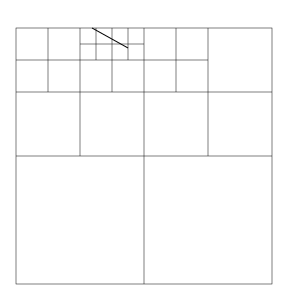
\includegraphics[width=5cm]{images/meshes/AMR/amr4}
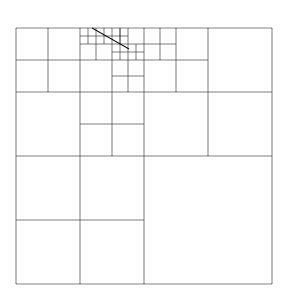
\includegraphics[width=5cm]{images/meshes/AMR/amr5}\\
\includegraphics[width=5cm]{images/meshes/AMR/amr6}
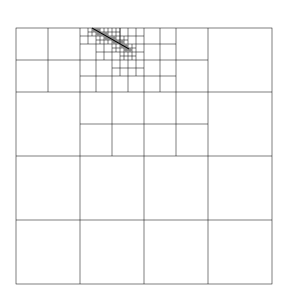
\includegraphics[width=5cm]{images/meshes/AMR/amr7}
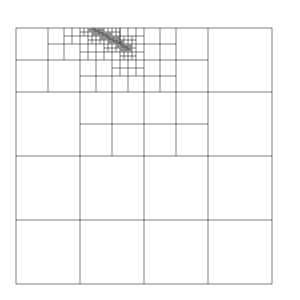
\includegraphics[width=5cm]{images/meshes/AMR/amr8}

\begin{tabular}{l|ccccccccc}
             & \# l0  & \# l1 & \# l2 & \# l3 & \# l4 & \# l5 & \# l6 & \# l7 & \# l8 \\ 
\hline\hline
max level= 0 & 1 & \\
max level= 1 & 0 & 4 & \\
max level= 2 & 0 & 3 & 4 \\
max level= 3 & 0 & 2 & 7 & 4\\
max level= 4 & 0 & 2 & 5 & 10 & 8 \\
max level= 5 & 0 & 1 & 8 & 12 & 11 & 20 \\ 
max level= 6 & 0 & 1 & 8 & 11 & 13 & 20 & 32 \\
max level= 7 & 0 & 0 & 11 & 14 & 15 & 23 & 37 & 60 \\
max level= 8 & 0 & 0 & 11 & 13 & 17 & 27 & 43 & 72 & 116 \\
\hline
\end{tabular}

\includegraphics[width=8cm]{images/meshes/AMR/amr_data1.pdf}
\includegraphics[width=8cm]{images/meshes/AMR/amr_data2.pdf}

In the particular case presented here, even though the inclusion in a short 
two-dimensional line, the total number of elements grows faster than the 
third power of the refinement level. While of course the total number 
of elements remains much smaller than the constant resolution counterpart, 
this observation tells us that authorising a unit increase of the maximum 
refinement level can have a substantial effect on the total number of elements.

\newpage

\noindent
\includegraphics[width=4cm]{images/meshes/AMR/amr_0}
\includegraphics[width=4cm]{images/meshes/AMR/amr_1}
\includegraphics[width=4cm]{images/meshes/AMR/amr_2}
\includegraphics[width=4cm]{images/meshes/AMR/amr_3}\\
\includegraphics[width=4cm]{images/meshes/AMR/amr_4}
\includegraphics[width=4cm]{images/meshes/AMR/amr_5}
\includegraphics[width=4cm]{images/meshes/AMR/amr_6}
\includegraphics[width=4cm]{images/meshes/AMR/amr_7}


\includegraphics[width=5cm]{images/meshes/AMR/amr_data3.pdf}
\includegraphics[width=5cm]{images/meshes/AMR/amr_data4.pdf}
\includegraphics[width=5cm]{images/meshes/AMR/amr_data5.pdf}






%.......................................
\subsubsection{Conformal Mesh Refinement}

\Literature: \cite{vaks15}\cite{kott05}


%.......................................
\subsubsection{Meshes in an annulus}


\begin{center}
\includegraphics[width=7cm]{images/meshes/brhv08}
\includegraphics[width=7cm]{images/meshes/brva07a}\\
{\scriptsize The quadratic finite element mesh as used in \cite{brhv08,brva07a}}
\end{center}


%.......................................
\subsubsection{Meshes in a hollow sphere}

The cubed sphere \cite{roip96}

The Citcom mesh  \cite{thie18}

WRITE MORE!!
 %-----------------------------------
%\newpage %----------------------------------------------------------------------------------------
%\section{Visco-Plasticity} 
\Literature: \cite{mumc03,chpe15,momu06,muso11}

\subsubsection{Tensor invariants}\label{sec:invariants}

Before we dive into the world of nonlinear rheologies it is necessary to introduce the concept of tensor 
invariants since they are needed further on. \index{general}{Tensor Invariant}
Unfortunately there are many different notations used in the literature and these can prove to be 
confusing. Note that we only consider symmetric tensors in what follows.

\index{general}{Moment Invariant}
Given a tensor $\bm{T}$,  one can compute its (moment) invariants as follows \cite[p.339]{reddybook2}: 
\begin{itemize}
\item first invariant:
\begin{eqnarray}
{\cal I}_1({\bm T})|^{2D} &=& Tr[\bm{T}] = T_{xx} + T_{yy} \nonumber\\
{\cal I}_1({\bm T})|^{3D} &=& Tr[\bm{T}] = T_{xx} + T_{yy} + T_{zz} 
\end{eqnarray}
\item second invariant:
\begin{eqnarray}
{\cal I}_2({\bm T})|^{2D} &=& \frac{1}{2} Tr[{\bm T}\cdot{\bm T}] = \frac{1}{2} \sum_{ij} T_{ij} T_{ji} = \frac{1}{2} (T_{xx}^2 + T_{yy}^2) + T_{xy}^2 \nonumber\\
{\cal I}_2({\bm T})|^{3D} &=& \frac{1}{2} Tr[{\bm T}\cdot{\bm T}] = \frac{1}{2} \sum_{ij} T_{ij} T_{ji} = \frac{1}{2} (T_{xx}^2 + T_{yy}^2 + T_{yy}^2) + T_{xy}^2 + T_{xz}^2 + T_{yz}^2 
\end{eqnarray}
\item third invariant: 
\begin{equation}
{\cal I}_3({\bm T}) = \frac{1}{3} Tr[{\bm T}\cdot{\bm T}\cdot {\bm T}]  = \frac{1}{3}\sum_i\sum_j \sum_k T_{ij} T_{jk} T_{ki} 
\end{equation}
\end{itemize}
These definitions are to be found in Appendix A.2 of \cite{zita2}.
 

\subsubsection{Stress invariants}\label{sec:stress_invariants}

The implementation of the plasticity criterions relies essentially 
on the second invariants of the (deviatoric) stress ${\bm \tau}$ 
and the (deviatoric) strainrate tensors $\dot{\bm \varepsilon}$:

\begin{eqnarray}
{\cal I}_2({\bm \tau})|^{2D}            
&=& \frac{1}{2} ( \tau_{xx}^2 + \tau_{yy}^2  ) + \tau_{xy}^2   \nonumber\\
&=& \frac{1}{4} (\sigma_{xx} - \sigma_{yy})^2 + \sigma_{xy}^2 \nonumber\\
\nonumber\\
{\cal I}_2({\bm \tau})|^{3D}            
&=&\frac{1}{2}(\tau_{xx}^2 + \tau_{yy}^2 + \tau_{zz}^2 ) + \tau_{xy}^2 + \tau_{xz}^2 + \tau_{yz}^2  \nonumber\\
&=&\frac{1}{6}\left[(\sigma_{xx}-\sigma_{yy})^2 + (\sigma_{yy}-\sigma_{zz})^2 + (\sigma_{xx}-\sigma_{zz})^2 \right] 
   + \sigma_{xy}^2 + \sigma_{xz}^2 + \sigma_{yz}^2 \nonumber \\
\nonumber\\
{\cal I}_2(\dot{\bm{\varepsilon}}^d)|^{2D} 
&=& \frac{1}{2} \left[ (\dot{\varepsilon}_{xx}^d)^2 + (\dot{\varepsilon}_{yy}^d)^2  \right] + (\dot{\varepsilon}_{xy}^d)^2  \nonumber\\
           &=& \frac{1}{2} \left[ 
               \frac{1}{4}(\dot{\varepsilon}_{xx} - \dot{\varepsilon}_{yy})^2 + \frac{1}{4}(\dot{\varepsilon}_{yy} - \dot{\varepsilon}_{xx})^2 
               \right] + \dot{\varepsilon}_{xy}^2  \nonumber\\
           &=& \frac{1}{4} (\dot{\varepsilon}_{xx} - \dot{\varepsilon}_{yy})^2  + \dot{\varepsilon}_{xy}^2  \nonumber\\
\nonumber\\
{\cal I}_2(\dot{\bm{\varepsilon}}^d)|^{3D} 
&=& \frac{1}{2} \left[ (\dot{\varepsilon}_{xx}^d)^2 + (\dot{\varepsilon}_{yy}^d)^2 + (\dot{\varepsilon}_{zz}^d)^2   \right] 
+ (\dot{\varepsilon}_{xy}^d)^2  
+ (\dot{\varepsilon}_{xz}^d)^2  
+ (\dot{\varepsilon}_{yz}^d)^2  \nonumber\\
           &=& \frac{1}{6} \left[ (\dot{\epsilon}_{xx}-\dot{\epsilon}_{yy})^2 + (\dot{\epsilon}_{yy}-\dot{\epsilon}_{zz})^2 + (\dot{\epsilon}_{xx}-\dot{\epsilon}_{zz})^2 \right] 
               + \dot{\epsilon}_{xy}^2 + \dot{\epsilon}_{xz}^2 + \dot{\epsilon}_{yz}^2 \nonumber \\
\nonumber
\end{eqnarray}

Note that these (second) invariants are almost always used under a square root so we define:
\begin{mdframed}[backgroundcolor=blue!5]
\[
\tau_{e}=\sqrt{{\cal I}_2({\bm \tau})}
\quad\quad
\quad\quad
\dot{\varepsilon}_{e}=\sqrt{{\cal I}_2(\dot{\bm \varepsilon}^d)}
\]
\end{mdframed}
Note that these quantities have the same dimensions as their tensor counterparts, i.e. Pa for stresses and s$^{-1}$ for strain rates.

If the stress tensor is such that it is diagonal, i.e.
\[
{\bm \sigma}= \left( \begin{array}{ccc}
\sigma_1 & 0 & 0 \\
0 & \sigma_2 & 0 \\
0 & 0 & \sigma_3
\end{array}\right)
\qquad
{\rm and}
\qquad
{\bm \tau}= \left( \begin{array}{ccc}
\tau_1 & 0 & 0 \\
0 & \tau_2 & 0 \\
0 & 0 & \tau_3
\end{array}\right)
\]
then the invariants are 
\begin{eqnarray}
{\cal I}_1({\bm \sigma}) &=& \sigma_1 + \sigma_2+ \sigma_3 \nonumber\\
{\cal I}_2({\bm \tau})|^{2D} &=& \frac{1}{4} (\sigma_{1} - \sigma_{2})^2 \nonumber\\
{\cal I}_2({\bm \tau})|^{3D} &=& \frac{1}{6}\left[(\sigma_{1}-\sigma_{2})^2 + (\sigma_{2}-\sigma_{3})^2 
+ (\sigma_{1}-\sigma_{3})^2 \right] \\ 
{\cal I}_3({\bm \tau}) 
&=& \frac{1}{3} Tr[{\bm T}\cdot{\bm T}\cdot {\bm T}]  \nn\\
&=& \frac{1}{3} Tr
\left[
\left(
\begin{array}{ccc}
\tau_1 & 0 & 0 \\
0 & \tau_2 & 0 \\
0 & 0 & \tau_3 
\end{array}
\right)
\cdot
\left(
\begin{array}{ccc}
\tau_1 & 0 & 0 \\
0 & \tau_2 & 0 \\
0 & 0 & \tau_3 
\end{array}
\right)
\cdot
\left(
\begin{array}{ccc}
\tau_1 & 0 & 0 \\
0 & \tau_2 & 0 \\
0 & 0 & \tau_3 
\end{array}
\right)
\right] \nn\\
&=&  \frac{1}{3} Tr
\left(
\begin{array}{ccc}
\tau_1^3 & 0 & 0 \\
0 & \tau_2^3 & 0 \\
0 & 0 & \tau_3^3 
\end{array}
\right) \nn\\
&=& \frac{1}{3}(\tau_1^3+\tau_2^3+\tau_3^3) \nn\\
&=&  \frac{1}{3} [ 
(\sigma_1-{\cal I}_1({\bm \sigma})/3)^3+  
(\sigma_2-{\cal I}_1({\bm \sigma})/3)^3+
(\sigma_3-{\cal I}_1({\bm \sigma})/3)^3 ]   \nonumber\\ 
&=&  \frac{1}{3\cdot 27} [ 
(3\sigma_1-{\cal I}_1({\bm \sigma}))^3+  
(3\sigma_2-{\cal I}_1({\bm \sigma}))^3+
(3\sigma_3-{\cal I}_1({\bm \sigma}))^3 ]   \nonumber\\ 
&=& \frac{1}{81}
\left[
(2\sigma_1-\sigma_2-\sigma_3)^3+
(2\sigma_2-\sigma_1-\sigma_3)^3+
(2\sigma_3-\sigma_1-\sigma_2)^3
\right] 
\label{eq:3rdinvb} 
\end{eqnarray}
This formulation of the third invariant of ${\bm \tau}$ is used in \cite{wojc18}.


{\color{gray} 
One can prove that (REF?)\footnote{Near identical equations are to be found at 
\url{https://en.wikipedia.org/wiki/Cauchy_stress_tensor}} 
\begin{eqnarray}
{\cal I}_3({\bm \tau}) 
&=& \frac{1}{27} \left( 2 {\cal I}_1({\bm \sigma})^3 + 
9 {\cal I}_1({\bm \sigma}) {\cal I}_2({\bm \sigma}) 
+27 {\cal I}_3({\bm \sigma})   \right) \nn\\
&=& det ({\bm\tau}) \nn\\
&=& \tau_1 \tau_2\tau_3 \nn\\
\end{eqnarray}

The third (deviatoric) stress invariant is given by: (VERIFY!!)
\begin{eqnarray}
{\cal I}_3({\bm \tau})|^{3D} 
&=&  \frac{1}{3} s_{xx} (s_{xx}^2 + 3  s_{xy}^2   + 3  s_{xz}^2  )     \nonumber\\
&+& \frac{1}{3} s_{yy} (3s_{xy}^2 +  s_{yy}^2   + 3  s_{yz}^2  )     \nonumber\\
&+& \frac{1}{3} s_{zz} ( 3 s_{xz}^2  + 3 s_{yz}^2 +s_{zz}^2)       \nonumber\\
&+& 2   s_{xy} s_{xz} s_{yz}   \nonumber \\
&=& s_1 s_2 s_3 \nonumber
\end{eqnarray}

}

%%%%%%%%%%%%%%%%%%%%%%%%%%%%%%%%%%%%%%%%%%%%%%%%%%%%%%%%%%%%%%%%%%%%%%%%%%%%%%%%%%%%%%%%%%%%%%%%%%%%
\subsubsection{Alternative principal stresses notations}\label{sec:altinv}

The principal stress of the stress tensor ${\bm \sigma}$ are $\sigma_1$, $\sigma_2$
and $\sigma_3$ with $\sigma_1 \geq \sigma_2 \geq \sigma_3$.
Following \cite{wojc18}, we start by stating that the intermediate principal 
stress can always be represented as a linear combination of two other stresses:
\begin{equation}
\sigma_2 = (1-b)\sigma_1 + b \sigma_3
\qquad
{\rm where}
\qquad
b = \frac{\sigma_1-\sigma_2}{\sigma_1-\sigma_3}\in [0,1]
\end{equation}
The quantity $b$ is called the principal stress ratio. \index{general}{Principal Stress Ratio}
Let us now introduce the maximum shear plane stresses $p$ and $q$ such that 
\begin{equation}
p=\frac{\sigma_1+\sigma_3}{2}
\qquad
q=\frac{\sigma_1-\sigma_3}{2}
\end{equation}
so that we have 
\begin{eqnarray}
\sigma_1 &=& p+q \\
\sigma_2 &=& p-aq \qquad a=2b-1 \in[-1,1] \\
\sigma_3 &=& p-q
\end{eqnarray}
The quantity $a$ is an equivalent measure of the principal stress ratio.
We can introduce $a,p,q$ in the invariants above:
\begin{eqnarray}
{\cal I}_1({\bm \sigma}) 
&=& \sigma_1 + \sigma_2 + \sigma_3 \nn\\
&=& p+q + p-aq + p-q \nn\\
&=& 3p -aq \\
{\cal I}_2({\bm \tau}) 
&=&\frac{1}{6}\left[(\sigma_{1}-\sigma_{2})^2 +(\sigma_{2}-\sigma_{3})^2 +(\sigma_{1}-\sigma_{3})^2\right]\nn\\ 
&=&\frac{1}{6}\left[(p+q-p+aq)^2 +(p-aq-p+q)^2 +(p+q-p+q)^2\right]\nn\\ 
&=&\frac{1}{6}\left[(q+aq)^2 +(-aq+q)^2 +(q+q)^2\right]\nn\\ 
&=&\frac{q^2}{6}\left[(1+a)^2 +(-a+1)^2 + 4 \right]\nn\\ 
&=&\frac{q^2}{6}\left[ 1+2a+a^2 +1 - 2a+a^2 + 4 \right]\nn\\ 
&=&\frac{q^2}{3}\left( a^2 +3 \right)
\end{eqnarray}
Using the definition of the third invariant of Eq.~\ref{eq:3rdinvb}:
\begin{eqnarray}
{\cal I}_3({\bm \tau}) 
&=& \frac{1}{81} \left[
(2\sigma_1-\sigma_2-\sigma_3)^3+
(2\sigma_2-\sigma_1-\sigma_3)^3+
(2\sigma_3-\sigma_1-\sigma_2)^3
\right] \nn\\
&=& \frac{1}{81} \left[
(2p+2q-p+aq-p+q)^3+
(2p-2aq-p-q-p+q)^3+
(2p-2q-p-q-p+aq)^3
\right] \nn\\
&=& \frac{1}{81} \left[ (2q+aq+q)^3+ (-2aq-q+q)^3+ (-2q-q+aq)^3 \right] \nn\\
&=& \frac{q^3}{81} \left[ (3+a)^3+ (-2a)^3+ (-3+a)^3 \right] \nn\\
&=& \frac{q^3}{81} \left[ 27 +9a + 3a^2 + a^3  -8a^3 -27 +9a -3a^2 + a^3 \right] \nn\\
&=& \frac{q^3}{81} \left( 18a  -6 a^3  \right) \nn\\
&=& \frac{2a q^3}{27} \left( 3 - a^2  \right) 
\end{eqnarray}
which is not exactly Eq.(14) of \cite{wojc18}!!

\begin{remark}
Wojciechowski \cite{wojc18} defines the Lode angle \index{general}{Lode Angle} 
as being the opposite of my definition in Eq.~\ref{eq:lodang}.
\end{remark}

Finally, we can show that 
\begin{eqnarray}
a 
&=& 2b-1 \nn\\
&=& 2 \frac{\sigma_1-\sigma_2}{\sigma_1-\sigma_3} -1 \nn\\
&=& 2 \frac{  -\frac{1}{\sqrt{3}}\sin \theta  + \cos \theta - \frac{2}{\sqrt{3}} \sin \theta }
{-\frac{1}{\sqrt{3}}\sin \theta  + \cos \theta +\frac{1}{\sqrt{3}}\sin \theta  + \cos \theta } -1 \nn\\
&=& \frac{ -\frac{1}{\sqrt{3}}\sin \theta  + \cos \theta - \frac{2}{\sqrt{3}}\sin\theta }{\cos \theta } -1 \nn\\
&=& -\frac{3}{\sqrt{3}} \frac{\sin\theta}{\cos\theta} \nn\\
&=& -\sqrt{3} \tan\theta
\end{eqnarray}
Here again we arrive at the opposite of Eq.16 of \cite{wojc18}. 

%%%%%%%%%%%%%%%%%%%%%%%%%%%%%%%%%%%%%%%%%%%%%%%%%%%%%%%%%%%%%%%%%%%%%%%%%%%%%%%%%%%%%%%%%%%%%%%%%%%%
\subsubsection{Scalar viscoplasticity}

This formulation is quite easy to implement. It is widely used, e.g. \cite{will92,thfb08,spmw16}, and relies on the assumption that 
a scalar quantity $\eta_p$ (the 'effective plastic viscosity') exists such that the deviatoric stress tensor 
\begin{equation}
{\bm \tau}=2\eta_p \dot{\bm\varepsilon} \label{eqscpl1}
\end{equation}
is bounded by some yield stress value $Y$.
From Eq. (\ref{eqscpl1}) it follows that $\underline{\tau}_{II}= 2\eta_p \dot{\underline{\varepsilon}}_{II}=Y$ which yields
\begin{mdframed}[backgroundcolor=blue!5]
\[
\eta_p = \frac{Y}{2 \dot{\underline{\varepsilon}}_{II}}
\]
\end{mdframed}
This approach has also been coined the Viscosity Rescaling Method (VRM) \cite{kacha04}. 
\index{general}{VRM} \index{general}{Viscosity Rescaling Method}

\improvement[inline]{insert here the rederivation 2.1.1 of spmw16}

It is at this stage important to realise that (i) in areas where the strainrate is low, the resulting effective viscosity will be large, and 
(ii) in areas where the strainrate is high, the resulting effective viscosity will be low. This is not without consequences since 
(effective) viscosity contrasts up to 8-10 orders of magnitude have been observed/obtained with this formulation and it makes the FE 
matrix very stiff, leading to (iterative) solver convergence issues.
In order to contain these viscosity contrasts one usually resorts to viscosity limiters $\eta_{min}$ and $\eta_{max}$ such that 
\[
\eta_{min} \leq \eta_p \leq \eta_{max}
\]
Caution must be taken when choosing both values as they may influence the final results.


\begin{mdframed}[backgroundcolor=green!5]
\begin{itemize}
\item[$\triangleright$] {\sl python\_codes/fieldstone\_indentor}
\end{itemize}
\end{mdframed}


%-------------------------------------------------
\subsubsection{About the yield stress value $Y$}

In geodynamics the yield stress value is often given as a simple function. 
It can be constant (in space and time) and in this case we are dealing with a von Mises plasticity yield criterion. 
\index{general}{von Mises}. We simply assume $Y_{vM}=C$ where $C$ is a constant cohesion independent of pressure, strainrate,
deformation history, etc ... \index{general}{Cohesion}

Another model is often used: the Drucker-Prager plasticity model. \index{general}{Drucker-Prager}
A friction angle $\phi$ is then introduced and the yield value $Y$ takes the form
\[
Y_{DP}=p \sin\phi + C \cos \phi
\]
and therefore depends on the pressure $p$. Because $\phi$ is with the range $[0^\circ,45^\circ]$, $Y$ is
found to increase with depth (since the lithostatic pressure often dominates the overpressure).

Note that a slightly modified verion of this plasticity model has been used: the total pressure $p$
is then replaced by the lithostatic pressure $p_{lith}$.




%-------------------------------------------------
\subsubsection{Work in progress}

\Literature \cite{zico74,zigo74,zico74b,zien75,corm75,zigo75,zihl75,zijo78,vidm82,vidm84,vede84,zivt85,vimd86}
\cite{wasd97,debo88,debo01,hesd02,bewv11,mumg10,leor89,sccm13,desm93,demu92,debo91,shmv16}
\cite{modm01}\cite{baji02}
\cite{modm02}

Note that \cite{vidm82,vidm84,vimd86,zivt85} use the following formulation which they attribute to \cite{zijo78}:
\[
\eta_{eff} = \frac{c + (\dot{\varepsilon}_e / \gamma)^{1/n}}{ \dot{\varepsilon}_e }
\] 
For a perfectly plastic flow law, $\gamma \rightarrow \infty$ and then 
\[
\eta_{eff} = \frac{c}{ \dot{\varepsilon}_e }
\] 
and when when $c=0$ then the effective viscosity is essentially of the power law type.
Also, when $n=1$ the formulation becomes identical to the v-vp formulation (when the max viscosity is infinite) and with $1/\gamma=\eta_{min}$.





 %-------------------------------------------
\newpage %-----------------------------------------------------------------------------------------
\section{Pressure smoothing/filtering/recovery for $Q_1\times P_0$ elements \label{psmoothing}} 
It has been widely documented that the use of the $Q_1 \times P_0$ element is 
not without problems. Aside from the 
consequences it has on the FE matrix properties, we will here focus on another unavoidable side effect: 
the spurious pressure checkerboard modes. 
\index{general}{Pressure Smoothing} 
\index{general}{Checkerboard mode}

These modes have been thoroughly analysed decades ago, see for instance
Hughes \etal (1979)\cite{hulb79}, 
Sani \etal (1981) \cite{sagl81a,sagl81b},
Griffiths \& Silvester (1994) \cite{grsi94}.
They can be filtered out(Chen (1995)  \cite{chpc95}) 
or simply smoothed (Lee \etal (1979) \cite{legs79}), as we will see later.
Nodes on edges and corners may need special treatment as documented in Sani \etal \cite{sagl81a} or
Lee \etal (1979) \cite{legs79}.
The list of 8 schemes is not exhaustive with regards to the above mentioned publications. 
There has been considerable amount of work on the topic and this section is 
unfortunately not representing the literature appropriately.

\mscthesis: Get relevant literature, digest it, implement all variants in \stone 12.
 \index{general}{MSc Thesis} 


On the following figure (a,b), pressure fields for the lid driven cavity experiment 
are presented for both an even and un-even number of elements. We see that 
the amplitude of the modes can sometimes be so large that the 'real' pressure signal is 
not visible under the checkerboard and that something as simple as the number of elements in the 
domain can trigger those or not at all.

\begin{center}
a)\includegraphics[width=4cm]{images/checkerboard/p_el}
\includegraphics[width=4cm]{images/checkerboard/p_el_33x33}
b)\includegraphics[width=5cm]{images/checkerboard/press_doneahuerta}
c)\includegraphics[width=7cm]{images/checkerboard/douarpunch}\\
{\captionfont a) element pressure for a 32x32 grid and for a 33x33 grid;\\ 
b) image from \cite[p307]{dohu03} for a manufactured solution;
c) elemental pressure and smoothed pressure for the punch experiment \cite{thfb08}}
\end{center}

%----------------------------------------------------------------------
\paragraph{Scheme 1}.

The easiest post-processing step that can be used (especially when a regular grid is used) 
is explained in Thieulot \etal (2008) \cite{thfb08}: "The element-to-node interpolation is performed by
averaging the elemental values from elements common to each node; 
the node-to-element interpolation is performed
by averaging the nodal values element-by-element. This
method is not only very efficient but produces a smoothing
of the pressure that is adapted to the local density of the
octree. Note that these two steps can be repeated until a
satisfying level of smoothness (and diffusion) of the pressure field is attained."


\begin{center}
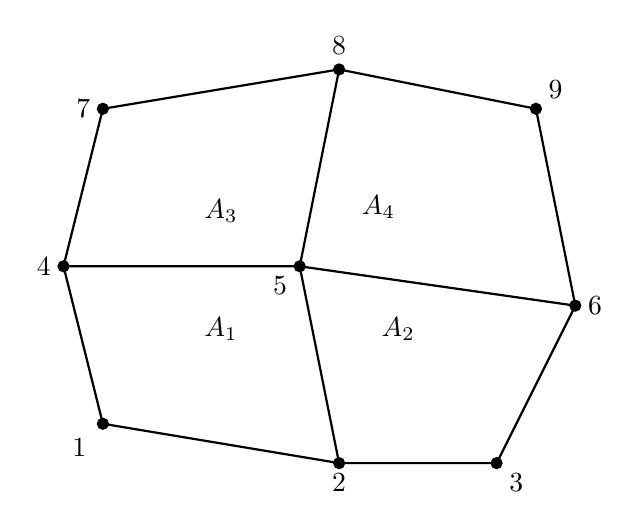
\begin{tikzpicture}
%\draw[fill=gray!5,gray!5](0,0) rectangle (9,7);
%\draw[step=0.5cm,gray,very thin] (0,0) grid (9,7); %background grid
\draw[thick](1.5,1.5) -- (4.5,1) -- (6.5,1) -- (7.5,3) -- (7,5.5) -- (4.5,6) --(1.5,5.5) -- (1,3.5) -- cycle;  
\draw[thick](4.5,1)--(4,3.5)--(4.5,6);
\draw[thick](1,3.5)--(4,3.5)--(7.5,3);
\draw[black,fill=black] (1.5,1.5) circle (2pt); \node[] at (1.2,1.2){1}; %1
\draw[black,fill=black] (4.5,1)   circle (2pt); \node[] at (4.5,0.75){2}; %2
\draw[black,fill=black] (6.5,1)   circle (2pt); \node[] at (6.75,0.75){3}; %3
\draw[black,fill=black] (1,3.5)   circle (2pt); \node[] at (0.75,3.5){4}; %4
\draw[black,fill=black] (4,3.5)   circle (2pt); \node[] at (3.75,3.25){5}; %5
\draw[black,fill=black] (7.5,3)   circle (2pt); \node[] at (7.75,3){6}; %6
\draw[black,fill=black] (1.5,5.5) circle (2pt); \node[] at (1.25,5.5){7}; %7
\draw[black,fill=black] (4.5,6)   circle (2pt); \node[] at (4.5,6.3){8}; %8
\draw[black,fill=black] (7,5.5)   circle (2pt); \node[] at (7.25,5.75){9}; %9
%\draw[thin,dashed](1,3.5)--(4.5,1)--(7.5,3)--(4.5,6)--cycle;
\node[] at (3,2.7){$A_1$}; %8
\node[] at (5.25,2.7){$A_2$}; %8
\node[] at (5,4.25){$A_4$}; %8
\node[] at (3,4.2){$A_3$}; %8
\end{tikzpicture}
\end{center}
\[
q_5^{(1)} = \frac{1}{4}\sum_{e=1}^4 p_e
\] 

In the codes which rely on the $Q_1 \times P_0$ element, the (elemental) pressure
is simply defined as 
\begin{lstlisting}
p=np.zeros(nel,dtype=np.float64)  
\end{lstlisting}
while the nodal pressure is then defined as\footnote{In virtually all stones $p$
stands for the 'raw' pressure and $q$ stands for its projection onto the velocity mesh.} 
\begin{lstlisting}
q=np.zeros(nnp,dtype=np.float64)  
\end{lstlisting}
The element-to-node algorithm is then simply (in 2D):

\begin{lstlisting}
count=np.zeros(nnp,dtype=np.int32)  
for iel in range(0,nel):
    q[icon[0,iel]]+=p[iel]
    q[icon[1,iel]]+=p[iel]
    q[icon[2,iel]]+=p[iel]
    q[icon[3,iel]]+=p[iel]
    count[icon[0,iel]]+=1
    count[icon[1,iel]]+=1
    count[icon[2,iel]]+=1
    count[icon[3,iel]]+=1
q=q/count
\end{lstlisting}



%----------------------------------------------------------------------
\paragraph{Schemes 2,3}.

{\sl Schemes 2,3} are very similar and are presented in Sani \etal (1981) \cite{sagl81a,sagl81b}.
Scheme 2 uses the areas of the surrounding elements as weights for the arithmetic averaging
while scheme 3 uses the area of the triangles:

\begin{multicols}{2}

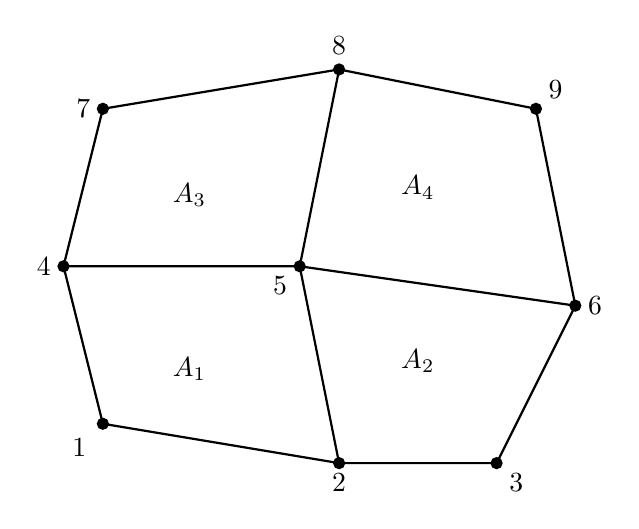
\begin{tikzpicture}
%\draw[fill=gray!5,gray!5](0,0) rectangle (9,7);
%\draw[step=0.5cm,gray,very thin] (0,0) grid (9,7); %background grid
\draw[thick](1.5,1.5) -- (4.5,1) -- (6.5,1) -- (7.5,3) -- (7,5.5) -- (4.5,6) --(1.5,5.5) -- (1,3.5) -- cycle;  
\draw[thick](4.5,1)--(4,3.5)--(4.5,6);
\draw[thick](1,3.5)--(4,3.5)--(7.5,3);
\draw[black,fill=black] (1.5,1.5) circle (2pt); \node[] at (1.2,1.2){1}; %1
\draw[black,fill=black] (4.5,1)   circle (2pt); \node[] at (4.5,0.75){2}; %2
\draw[black,fill=black] (6.5,1)   circle (2pt); \node[] at (6.75,0.75){3}; %3
\draw[black,fill=black] (1,3.5)   circle (2pt); \node[] at (0.75,3.5){4}; %4
\draw[black,fill=black] (4,3.5)   circle (2pt); \node[] at (3.75,3.25){5}; %5
\draw[black,fill=black] (7.5,3)   circle (2pt); \node[] at (7.75,3){6}; %6
\draw[black,fill=black] (1.5,5.5) circle (2pt); \node[] at (1.25,5.5){7}; %7
\draw[black,fill=black] (4.5,6)   circle (2pt); \node[] at (4.5,6.3){8}; %8
\draw[black,fill=black] (7,5.5)   circle (2pt); \node[] at (7.25,5.75){9}; %9
\node[] at (2.6,2.2){$A_1$}; %8
\node[] at (5.5,2.3){$A_2$}; %8
\node[] at (2.6,4.4){$A_3$}; %8
\node[] at (5.5,4.5){$A_4$}; %8
\end{tikzpicture}

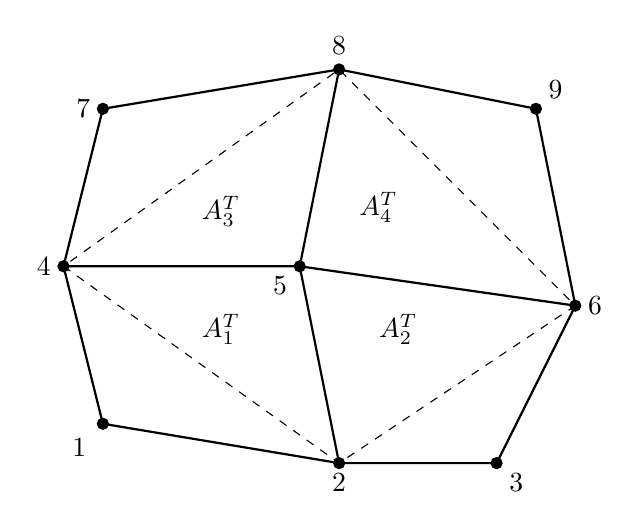
\begin{tikzpicture}
%\draw[fill=gray!5,gray!5](0,0) rectangle (9,7);
%\draw[step=0.5cm,gray,very thin] (0,0) grid (9,7); %background grid
\draw[thick](1.5,1.5) -- (4.5,1) -- (6.5,1) -- (7.5,3) -- (7,5.5) -- (4.5,6) --(1.5,5.5) -- (1,3.5) -- cycle;  
\draw[thick](4.5,1)--(4,3.5)--(4.5,6);
\draw[thick](1,3.5)--(4,3.5)--(7.5,3);
\draw[black,fill=black] (1.5,1.5) circle (2pt); \node[] at (1.2,1.2){1}; %1
\draw[black,fill=black] (4.5,1)   circle (2pt); \node[] at (4.5,0.75){2}; %2
\draw[black,fill=black] (6.5,1)   circle (2pt); \node[] at (6.75,0.75){3}; %3
\draw[black,fill=black] (1,3.5)   circle (2pt); \node[] at (0.75,3.5){4}; %4
\draw[black,fill=black] (4,3.5)   circle (2pt); \node[] at (3.75,3.25){5}; %5
\draw[black,fill=black] (7.5,3)   circle (2pt); \node[] at (7.75,3){6}; %6
\draw[black,fill=black] (1.5,5.5) circle (2pt); \node[] at (1.25,5.5){7}; %7
\draw[black,fill=black] (4.5,6)   circle (2pt); \node[] at (4.5,6.3){8}; %8
\draw[black,fill=black] (7,5.5)   circle (2pt); \node[] at (7.25,5.75){9}; %9
\draw[thin,dashed](1,3.5)--(4.5,1)--(7.5,3)--(4.5,6)--cycle;
\node[] at (3,2.7){$A_1^T$}; %8
\node[] at (5.25,2.7){$A_2^T$}; %8
\node[] at (5,4.25){$A_4^T$}; %8
\node[] at (3,4.2){$A_3^T$}; %8
\end{tikzpicture}

\end{multicols}




\[
q_5^{(2)} = \frac{\sum\limits_{e=1}^4 A_e p_e}{\sum\limits_{e=1}^4 A_e}
\qquad
\qquad
q_5^{(3)} = \frac{\sum\limits_{e=1}^4 A_e^T p_e}{\sum\limits_{e=1}^4 A_e^T}
\] 


\begin{remark} Although Schemes 1,2,3 are similar, scheme 1 is the simplest and fastest
to implement since the areas of neighbouring elements/triangles are not needed.
\end{remark}

\begin{remark} 
Schemes 1,2,3 are identical if all elements are rectangles of identical dimensions.
\end{remark}




%----------------------------------------------------------------------
\paragraph{Scheme 4} This scheme has been designed by me. 
It resembles the last three ones, but the weighing is in this case different.

Let us consider a 1D problem:
\begin{center}
\includegraphics[width=0.5\linewidth]{images/pressure_smoothing/newalgo.png}
\end{center}

Elemental pressures $p_1$ and $p_2$ corresponding to elements 1 and 2 respectively are known at
locations $x_1$ and $x_2$. The two elements have a different size, characterised in this case
by the distances $d_1$ and $d_2$ to their common edge.

The equation of the line passing through points $(x_1,p_1)$ and $(x_2,p_2)$ is 
\[
p(x)=\frac{p_2-p_1}{x_2-x_1}(x-x_1)+p_1
\]
The $x$ coordinate of the common edge is given by $x=x_1+d_1/2$, 
and since $x_2-x_1=(d_1+d_2)/2$, the 
pressure at this location writes:
\[
p(x_M)= \frac{p_2-p_1}{d_1+d_2}d_1+p_1 = \frac{\frac{p_1}{d_1} + \frac{p_2}{d_2}}{\frac{1}{d_1} + \frac{1}{d_2}}
\]
Extrapolating this formula to 2D, $d_1$ and $d_2$ are in fact the element volumes, so that
\[
q_5^{(4)} = 
\frac{\sum\limits_{j=1}^4 \frac{p_j^e}{A_j^e}}{\sum\limits_{j=1}^4 \frac{1}{A_j^e}}
=
\frac{
\frac{p_1^e}{A_1^e}+
\frac{p_2^e}{A_2^e}+
\frac{p_3^e}{A_3^e}+
\frac{p_4^e}{A_4^e}
}{
\frac{1}{A_1^e}+
\frac{1}{A_2^e}+
\frac{1}{A_3^e}+
\frac{1}{A_4^e}
}\]

There remains a problem, due to the presence of the boundary nodes for which 
the sums present in the above equation do not run up to 4. A boundary
node only has three neighbours and a corner node only two. Additional measures
are required for these nodes. 

\begin{center}
\includegraphics[width=0.5\linewidth]{images/pressure_smoothing/newalgo_corner.png}
\end{center}

The pressure value $p_N$ is obtained as follows:
\[
q_N = \frac{ 
 \frac{p_2^e}   {A_2^e}
+\frac{p_3^e}   {A_3^e}
+\frac{p_{2'}^e}{A_{2'}^e}
+\frac{p_{3'}^e}{A_{3'}^e}
}{
 \frac{1}{A_2^e}
+\frac{1}{A_3^e}
+\frac{1}{A_{2'}^e}
+\frac{1}{A_{3'}^e}
}
\]
The areas and pressures of the mirrored elements 2' and 3' are extrapolated from the areas of elements 2 and 6, and 3 and 7 respectively. 
Likewise the pressure $p_M$ at the corner node is obtained through the pressures of its surrounding elements.


%------------------------------------------------------------------------------
\paragraph{Scheme 5 - Least squares} This scheme is presented (among other places) in Lee \etal (1979)
\cite{legs79}. 
Let us start from the patch of 4 $Q_1$ elements counting 9 nodes: 

\begin{center}
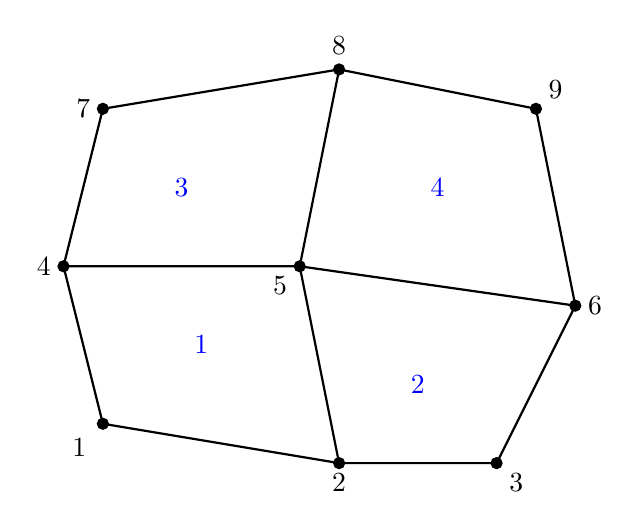
\begin{tikzpicture}
%\draw[fill=gray!5,gray!5](0,0) rectangle (9,7);
%\draw[step=0.5cm,gray,very thin] (0,0) grid (9,7); %background grid
\draw[thick](1.5,1.5) -- (4.5,1) -- (6.5,1) -- (7.5,3) -- (7,5.5) -- (4.5,6) --(1.5,5.5) -- (1,3.5) -- cycle;  
\draw[thick](4.5,1)--(4,3.5)--(4.5,6);
\draw[thick](1,3.5)--(4,3.5)--(7.5,3);

\node[] at (2.75,2.5) {\color{blue}1};
\node[] at (5.5,2) {\color{blue}2};
\node[] at (2.5,4.5) {\color{blue}3};
\node[] at (5.75,4.5) {\color{blue}4};

\draw[black,fill=black] (1.5,1.5) circle (2pt); \node[] at (1.2,1.2){1}; %1
\draw[black,fill=black] (4.5,1)   circle (2pt); \node[] at (4.5,0.75){2}; %2
\draw[black,fill=black] (6.5,1)   circle (2pt); \node[] at (6.75,0.75){3}; %3
\draw[black,fill=black] (1,3.5)   circle (2pt); \node[] at (0.75,3.5){4}; %4
\draw[black,fill=black] (4,3.5)   circle (2pt); \node[] at (3.75,3.25){5}; %5
\draw[black,fill=black] (7.5,3)   circle (2pt); \node[] at (7.75,3){6}; %6
\draw[black,fill=black] (1.5,5.5) circle (2pt); \node[] at (1.25,5.5){7}; %7
\draw[black,fill=black] (4.5,6)   circle (2pt); \node[] at (4.5,6.3){8}; %8
\draw[black,fill=black] (7,5.5)   circle (2pt); \node[] at (7.25,5.75){9}; %9

\end{tikzpicture}
\end{center}



We are looking for a field $q$ living on the nodes.
We build the quantity
\[
J=\iint_\Omega (q-p)^2 dV
\]
where $p$ is the elemental field. To make things clearer we split the integral into 
the sum of elemental integrals:
\[
J=
\iint_{\Omega_1} (q(x,y)-p_1)^2 dV+
\iint_{\Omega_2} (q(x,y)-p_2)^2 dV+
\iint_{\Omega_3} (q(x,y)-p_3)^2 dV+
\iint_{\Omega_4} (q(x,y)-p_4)^2 dV
\]
Inside each element the field $q(x,y)$ is given by a bilinear interpolation so that:
\begin{eqnarray}
J
&=& \iint_{\Omega_1} (\bN_1(x,y) q_1 + \bN_2(x,y)q_2 + \bN_5(x,y)q_5 + \bN_4(x,y)q_4 -p_1)^2 dV \nn\\
&+& \iint_{\Omega_2} (\bN_2(x,y) q_2 + \bN_3(x,y)q_3 + \bN_6(x,y)q_6 + \bN_5(x,y)q_5 -p_2)^2 dV \nn\\
&+& \iint_{\Omega_3} (\bN_4(x,y) q_4 + \bN_5(x,y)q_5 + \bN_8(x,y)q_8 + \bN_7(x,y)q_7 -p_3)^2 dV \nn\\
&+& \iint_{\Omega_4} (\bN_5(x,y) q_5 + \bN_6(x,y)q_6 + \bN_9(x,y)q_9 + \bN_8(x,y)q_8 -p_4)^2 dV 
\end{eqnarray}
where the $N_i$ functions are the basis functions (unusually expressed in $x,y$ coordinates).
The least square procedure looks for the set of $q_i$ such that 
\[
\frac{\partial J}{\partial q_i} =0 \qquad \forall i=1,...9
\]
and this yields 9 equations/constraints for 9 unknowns.
\begin{eqnarray}
\frac{\partial J}{\partial q_1} 
&=& \iint_{\Omega_1} 2 (\bN_1(x,y) q_1 + \bN_2(x,y)q_2 + \bN_5(x,y)q_5 + \bN_4(x,y)q_4 -p_1) \bN_1(x,y) dV \nn\\
\frac{\partial J}{\partial q_2}
&=& \iint_{\Omega_1} 2(\bN_1(x,y) q_1 + \bN_2(x,y)q_2 + \bN_5(x,y)q_5 + \bN_4(x,y)q_4 -p_1) \bN_2(x,y) dV \nn\\
&+& \iint_{\Omega_2} 2(\bN_2(x,y) q_2 + \bN_3(x,y)q_3 + \bN_6(x,y)q_6 + \bN_5(x,y)q_5 -p_2) \bN_2(x,y) dV \nn\\
\frac{\partial J}{\partial q_3}
&=& \iint_{\Omega_2} 2(\bN_2(x,y) q_2 + \bN_3(x,y)q_3 + \bN_6(x,y)q_6 + \bN_5(x,y)q_5 -p_2) \bN_3(x,y) dV \nn\\
\frac{\partial J}{\partial q_4}
&=& \iint_{\Omega_1} 2(\bN_1(x,y) q_1 + \bN_2(x,y)q_2 + \bN_5(x,y)q_5 + \bN_4(x,y)q_4 -p_1) \bN_4(x,y) dV \nn\\
&+& \iint_{\Omega_3} 2(\bN_4(x,y) q_4 + \bN_5(x,y)q_5 + \bN_8(x,y)q_8 + \bN_7(x,y)q_7 -p_3) \bN_4(x,y) dV \nn\\
\frac{\partial J}{\partial q_5}
&=& \iint_{\Omega_1} 2(\bN_1(x,y) q_1 + \bN_2(x,y)q_2 + \bN_5(x,y)q_5 + \bN_4(x,y)q_4 -p_1) \bN_5(x,y) dV \nn\\
&+& \iint_{\Omega_2} 2(\bN_2(x,y) q_2 + \bN_3(x,y)q_3 + \bN_6(x,y)q_6 + \bN_5(x,y)q_5 -p_2) \bN_5(x,y) dV \nn\\
&+& \iint_{\Omega_3} 2(\bN_4(x,y) q_4 + \bN_5(x,y)q_5 + \bN_8(x,y)q_8 + \bN_7(x,y)q_7 -p_3) \bN_5(x,y) dV \nn\\
&+& \iint_{\Omega_4} 2(\bN_5(x,y) q_5 + \bN_6(x,y)q_6 + \bN_9(x,y)q_9 + \bN_8(x,y)q_8 -p_4) \bN_5(x,y) dV \nn\\
\frac{\partial J}{\partial q_6}
&=& \iint_{\Omega_2} 2(\bN_2(x,y) q_2 + \bN_3(x,y)q_3 + \bN_6(x,y)q_6 + \bN_5(x,y)q_5 -p_2) \bN_6(x,y) dV \nn\\
&+& \iint_{\Omega_4} 2(\bN_5(x,y) q_5 + \bN_6(x,y)q_6 + \bN_9(x,y)q_9 + \bN_8(x,y)q_8 -p_4) \bN_6(x,y) dV \nn\\
\frac{\partial J}{\partial q_7}
&=& \iint_{\Omega_3} 2(\bN_4(x,y) q_4 + \bN_5(x,y)q_5 + \bN_8(x,y)q_8 + \bN_7(x,y)q_7 -p_3) \bN_7(x,y) dV \nn\\
\frac{\partial J}{\partial q_8}
&=& \iint_{\Omega_3} 2(\bN_4(x,y) q_4 + \bN_5(x,y)q_5 + \bN_8(x,y)q_8 + \bN_7(x,y)q_7 -p_3) \bN_8(x,y)dV \nn\\
&+& \iint_{\Omega_4} 2(\bN_5(x,y) q_5 + \bN_6(x,y)q_6 + \bN_9(x,y)q_9 + \bN_8(x,y)q_8 -p_4) \bN_8(x,y)dV \nn\\ 
\frac{\partial J}{\partial q_9}
&=& \iint_{\Omega_4} 2(\bN_5(x,y) q_5 + \bN_6(x,y)q_6 + \bN_9(x,y)q_9 + \bN_8(x,y)q_8 -p_4) \bN_9(x,y)dV 
\end{eqnarray}
The factor 2 are removed and the terms $\int p_i N_j $ are known so they end up in the right hand side.
\begin{eqnarray}
 \iint_{\Omega_1} (\bN_1 \bN_1 q_1 + \bN_1 \bN_2 q_2 + \bN_1 \bN_5 q_5 + \bN_1 \bN_4 q_4) dV 
&=& \iint_{\Omega_1} p_1 N_1 dV \nn\\
 \iint_{\Omega_1} (\bN_2 \bN_1 q_1 + \bN_2 \bN_2 q_2 + \bN_2 \bN_5 q_5 + \bN_2 \bN_4 q_4) dV \nn\\
+\iint_{\Omega_2} (\bN_2 \bN_2 q_2 + \bN_3 \bN_2 q_3 + \bN_6 \bN_2 q_6 + \bN_5 \bN_2 q_5) dV 
&=& \iint_{\Omega_1} p_1N_2 dV + \iint_{\Omega_2}  p_2 \bN_2 dV \nn\\
\nn\\
\dots &=& \dots \nn\\
\nn\\
 \iint_{\Omega_4} (\bN_9\bN_5 q_5 + \bN_9\bN_6q_6 + \bN_9\bN_9q_9 + \bN_9\bN_8q_8) dV &=&  \iint_{\Omega_4} p_4 \bN_9 dV 
\end{eqnarray}

The mass matrices corresponding to the four elements are 
\[
{\bm M}_1 = \int_{\Omega_1} \left( \begin{array}{cccc}
 \bN_1 \bN_1 & \bN_1 \bN_2 & \bN_1 \bN_5 & \bN_1 \bN_4 \\
 \bN_2 \bN_1 & \bN_2 \bN_2 & \bN_2 \bN_5 & \bN_2 \bN_4 \\
 \bN_5 \bN_1 & \bN_5 \bN_2 & \bN_5 \bN_5 & \bN_5 \bN_4 \\
 \bN_4 \bN_1 & \bN_4 \bN_2 & \bN_4 \bN_5 & \bN_4 \bN_4 
\end{array}\right) dV
\qquad
{\bm M}_2 = \int_{\Omega_2} \left( \begin{array}{cccc}
 \bN_2 \bN_2 & \bN_2 \bN_3 & \bN_2 \bN_6 & \bN_2 \bN_5 \\
 \bN_3 \bN_2 & \bN_3 \bN_3 & \bN_3 \bN_6 & \bN_3 \bN_5 \\
 \bN_6 \bN_2 & \bN_6 \bN_3 & \bN_6 \bN_6 & \bN_6 \bN_5 \\
 \bN_5 \bN_2 & \bN_5 \bN_3 & \bN_5 \bN_6 & \bN_5 \bN_5 
\end{array}\right) dV
\]
\[
{\bm M}_3 = \int_{\Omega_3} \left( \begin{array}{cccc}
 \bN_4 \bN_4 & \bN_4 \bN_5 & \bN_4 \bN_8 & \bN_4 \bN_7 \\
 \bN_5 \bN_4 & \bN_5 \bN_5 & \bN_5 \bN_8 & \bN_5 \bN_7 \\
 \bN_8 \bN_4 & \bN_8 \bN_5 & \bN_8 \bN_8 & \bN_8 \bN_7 \\
 \bN_7 \bN_4 & \bN_7 \bN_5 & \bN_7 \bN_8 & \bN_7 \bN_7 
\end{array}\right) dV
\qquad
{\bm M}_4 = \int_{\Omega_4} \left( \begin{array}{cccc}
 \bN_5 \bN_5 & \bN_5 \bN_6 & \bN_5 \bN_9 & \bN_5 \bN_8 \\
 \bN_6 \bN_5 & \bN_6 \bN_6 & \bN_6 \bN_9 & \bN_6 \bN_8 \\
 \bN_9 \bN_5 & \bN_9 \bN_6 & \bN_9 \bN_9 & \bN_9 \bN_8 \\
 \bN_8 \bN_5 & \bN_8 \bN_6 & \bN_8 \bN_9 & \bN_8 \bN_8 
\end{array}\right) dV
\]
so that the 9 equations above are actually the result of the assembly process of these four 
elemental systems:
\[
\left( \iint_{\Omega_e} \vec{\bN}^T\vec{\bN} dV \right) \cdot \vec{q}_e = \iint_{\Omega_i} \vec{\bN}^T p_e dV 
\qquad\qquad e=1,2,3,4
\]


%------------------------------------------------------------------------------
\paragraph{Scheme 6 - Consistent pressure recovery}

The is the method presented in Zienkiewicz \& Nakazawa (1982) \cite{zina82}. In the second part 
of this publication the authors wish to establish a simple and effective numerical method to calculate 
variables eliminated by the penalisation process. 
The method involves an additional finite element solution for the nodal pressures using 
the same finite element basis and numerical quadrature as used for the velocity.

Let us start with\footnote{I here voluntarily use $q$ instead of $p$}:
\[
q = -\lambda \vec\nabla\cdot \vec\upnu
\]
We are going to treat this equation as any other PDE in the context of the FE method, i.e. 
we are going to establish its weak form. 
We assume that the pressure is given inside an element by
\[
q(x,y) = \sum_{i=1}^4 \bN_i(x,y) q_i = \vec{\bN} \cdot \vec{q}
\]
and the velocity:
\[
\vec\upnu = (u,v) 
\qquad 
\qquad 
u(x,y)  = \sum_{i=1}^4 \bN_i(x,y) u_i
\qquad 
\qquad 
v(x,y)  = \sum_{i=1}^4 \bN_i(x,y) v_i
\]
where the $\bN_i$ are the $Q_1$ basis functions and $q_i$ are the sought after nodal values. 
We multiply the equation above by a $Q_1$ basis function $\bN_i$ and integrate over the whole domain:
\[
\iint_\Omega \bN_i(x,y) q(x,y) \; dxdy 
= -\lambda \iint_\Omega \bN_i \vec\nabla\cdot \vec\upnu  \; dx dy
\]
As before we now focus on the above expression inside a single element $e$:
\[
\iint_{\Omega_e} \bN_i(x,y) q(x,y) \; dxdy = -\lambda \iint_{\Omega_e} \bN_i \vec\nabla\cdot \vec\upnu \; dx dy
\]
After $\bN_i \rightarrow \vec{\bN}=(\bN_1,\bN_2,\bN_3,\bN_4)^T$, the left hand side term becomes:
\[
\iint _{\Omega_e} \vec{\bN}^T q(x,y) \; dxdy 
=
\iint _{\Omega_e} \vec{\bN}^T \vec{\bN} \cdot \vec{q} \; dxdy 
=
\left(\underbrace{\iint _{\Omega_e} \vec{\bN}^T \vec{\bN} dxdy}_{{\bm M}_e} \right) \cdot \vec{q}  
\]
where ${\bm M}_e$ is the elemental mass matrix.
We now turn to the right hand side. We have
\[
\vec\nabla\cdot \vec\upnu
= \frac{\partial u}{\partial x}+\frac{\partial v}{\partial y}
= \sum_i \frac{\partial \bN_i}{\partial x} u_i + \sum_i \frac{\partial \bN_i}{\partial y} v_i 
\]
We here too define $\vec{V}_e=(u_1,v_1,u_2,v_2,u_3,v_3,u_4,v_4)^T$ so that 

\begin{eqnarray}
&& \iint_{\Omega_e} \vec{\bN} {\vec \nabla}\cdot {\vec \upnu} \; dV \nn\\
&=& \iint_{\Omega_e} \vec{\bN}^T \sum_{i=1}^{4} 
\left( \frac{\partial \bN_i}{\partial x} u_i + \frac{\partial \bN_i}{\partial y} v_i 
\right)  
dV \nonumber\\
&=& 
\iint_{\Omega_e} 
\left(
\begin{array}{c}
\bN_1 \left(
\sum\limits_{i=1}^{4} \frac{\partial \bN_i}{\partial x} u_i +
\sum\limits_{i=1}^{4} \frac{\partial \bN_i}{\partial y} v_i \right) \\
\bN_2 \left(
\sum\limits_{i=1}^{4} \frac{\partial \bN_i}{\partial x} u_i +
\sum\limits_{i=1}^{4} \frac{\partial \bN_i}{\partial y} v_i \right) \\
\bN_3 \left(
\sum\limits_{i=1}^{4} \frac{\partial \bN_i}{\partial x} u_i +
\sum\limits_{i=1}^{4} \frac{\partial \bN_i}{\partial y} v_i \right) \\
\bN_4 \left(
\sum\limits_{i=1}^{4} \frac{\partial \bN_i}{\partial x} u_i +
\sum\limits_{i=1}^{4} \frac{\partial \bN_i}{\partial y} v_i \right) 
\end{array}
\right) dV \nonumber \\  %%%%%%%%%%%%%%%%%%%%%%%%%%
&=& 
\int_{\Omega_e} 
\left(
\begin{array}{ccc}
{\bN}_1& {\bN}_1 &  0 \\\\
{\bN}_2& {\bN}_2 &  0 \\\\
{\bN}_3& {\bN}_3 &  0 \\\\
{\bN}_4& {\bN}_4 &  0 
\end{array}
\right)
\cdot
\left(
\begin{array}{c}
\sum\limits_i \frac{\partial \bN_i}{\partial x} u_i \\ \\
\sum\limits_i \frac{\partial \bN_i}{\partial y} v_i \\ \\
\sum\limits_i (\frac{\partial \bN_i}{\partial y} u_i\! +\! \frac{\partial \bN_i}{\partial x} v_i) 
\end{array}
\right)
\; dV \nonumber\\ %%%%%%%%%%%%%%%%%%%%%%%%%%
&=& 
\int_{\Omega_e} 
\underbrace{
\left(
\begin{array}{cccccc}
{\bN}_1 & {\bN}_1 &  0 \\
{\bN}_2 & {\bN}_2 &  0 \\
{\bN}_3 & {\bN}_3 &  0 \\
{\bN}_4 & {\bN}_4 &  0 
\end{array}
\right)
}_{{\bm N}}
\cdot
\underbrace{
\left(\begin{array}{cccccccc}
\partial_x \bN_1 & 0 &  
\partial_x \bN_2 & 0 &  
\partial_x \bN_3 & 0 &  
\partial_x \bN_4 & 0 \\ \\
0 & \partial_y \bN_1 &   
0 & \partial_y \bN_2 &   
0 & \partial_y \bN_3 &   
0 & \partial_y \bN_4 \\ \\
\partial_y \bN_1 & \partial_x \bN_1 &  
\partial_y \bN_2 & \partial_x \bN_2 &  
\partial_y \bN_3 & \partial_x \bN_3 &  
\partial_y \bN_4 & \partial_x \bN_4 
\end{array}\right)}_{{\bm B}}
\cdot \vec{V}_e
\; dV  \nonumber \\
&=& 
\left(\int_{\Omega_e} {\bm N} \cdot {\bm B} \; dV \right) \cdot \vec{V}_e \nonumber\\
&=& -\G_e^T \cdot {\vec V}_e
\end{eqnarray}

After assembly we arrive at
\[
{\bm M} \cdot \vec{q} = \lambda \G^T \cdot {\vec V} 
\qquad
\text{with}
\qquad
\G_e = -\int_{\Omega_e} {\bm N} \cdot {\bm B} \; dV
\]
where ${\bm M}$ is the global mass matrix, $\vec{q}$ the vector of all 
nodal pressures, $\G$ the discrete gradient matrix and $\vec{V}$
the (velocity) solution vector. 
The system can be easily solved since the mass matrix is a friendly matrix.
The vector ${\vec q}$ contains the nodal pressure values directly, with 
no need for a smoothing scheme! 

\begin{remark}
Very importantly, the mass matrix ${\bm M}$ is to be evaluated at the full integration points, 
while the constraint part (the right hand side of the equation) is to be evaluated at 
the reduced integration point, i.e. in the middle of the element.  
\end{remark}

\begin{remark}
As noted in \cite{zina82}, it is interesting to note that when linear elements are used 
and the lumped matrices are used for the ${\bm M}$ the resulting algebraic equation is identical 
to the smoothing scheme 1 only if a uniform square finite element 
mesh is used. In this respect this method is expected to yield different results when elements 
are not square or even rectangular.
\end{remark}

\begin{remark}
The third column of the matrix ${\bm N}$
and the last line of the ${\bm B}$ matrix could be removed altogether.
If your code is based on the mixed formulation, then you already 
have built matrix $\G$ so you can easily re-use this piece of code 
to compute $\G$ again, this time with a reduced integration quadrature.
If you are using the penalty formulation then you need to program 
all from scratch and then simply do away with these unnecessary terms, or 
you can direcly build the rhs as $\int_{\Omega_e} \vec{\bN}^T p_e$ (assuming
you have previously computed the pressure in the middle of each element 
by means of $p=-\lambda\vec\nabla\cdot\vec\upnu$).
\end{remark}

\begin{remark}
This  scheme is identical to the least square scheme!
\end{remark}


%--------------------------------------------------------------
\paragraph{Scheme 7}

Same as scheme 6, but with lumped mass matrix.  


%--------------------------------------------------------------
\paragraph{Scheme 8 - bilinear interpolation} Let us assume that the centers of the 
four elements make a $Q_1$ quadrilateral element, as shown on this figure:


\begin{center}
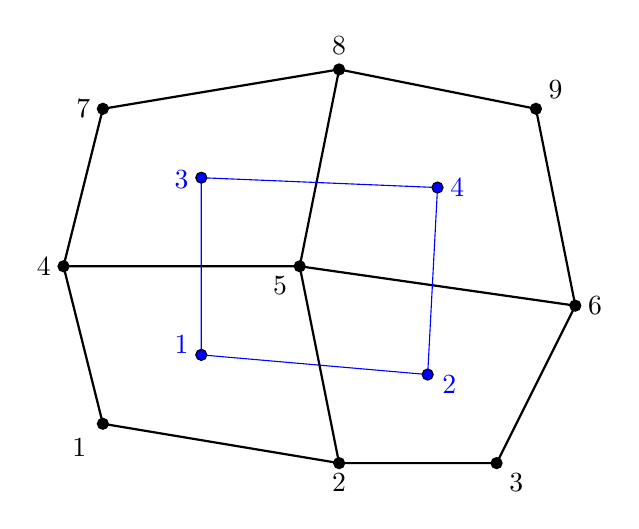
\begin{tikzpicture}
%\draw[fill=gray!5,gray!5](0,0) rectangle (9,7);
%\draw[step=0.5cm,gray,very thin] (0,0) grid (9,7); %background grid
\draw[thick](1.5,1.5) -- (4.5,1) -- (6.5,1) -- (7.5,3) -- (7,5.5) -- (4.5,6) --(1.5,5.5) -- (1,3.5) -- cycle;  
\draw[thick](4.5,1)--(4,3.5)--(4.5,6);
\draw[thick](1,3.5)--(4,3.5)--(7.5,3);

\draw[black,fill=blue] (2.75,2.375) circle (2pt); 
\node[] at (2.5,2.5) {\color{blue}1};
\draw[black,fill=blue] (5.625,2.125) circle (2pt); 
\node[] at (5.9,2) {\color{blue}2};
\draw[black,fill=blue] (5.75,4.5) circle (2pt); 
\node[] at (2.5,4.6) {\color{blue}3};
\draw[black,fill=blue] (2.75,4.625) circle (2pt); 
\node[] at (6,4.5) {\color{blue}4};

\draw[black,fill=black] (1.5,1.5) circle (2pt); \node[] at (1.2,1.2){1}; %1
\draw[black,fill=black] (4.5,1)   circle (2pt); \node[] at (4.5,0.75){2}; %2
\draw[black,fill=black] (6.5,1)   circle (2pt); \node[] at (6.75,0.75){3}; %3
\draw[black,fill=black] (1,3.5)   circle (2pt); \node[] at (0.75,3.5){4}; %4
\draw[black,fill=black] (4,3.5)   circle (2pt); \node[] at (3.75,3.25){5}; %5
\draw[black,fill=black] (7.5,3)   circle (2pt); \node[] at (7.75,3){6}; %6
\draw[black,fill=black] (1.5,5.5) circle (2pt); \node[] at (1.25,5.5){7}; %7
\draw[black,fill=black] (4.5,6)   circle (2pt); \node[] at (4.5,6.3){8}; %8
\draw[black,fill=black] (7,5.5)   circle (2pt); \node[] at (7.25,5.75){9}; %9

\draw[blue](2.75,2.375)--(5.625,2.125)--(5.75,4.5)--(2.75,4.625)--cycle;
\end{tikzpicture}
\end{center}




The values at the corners are $p_1$,
$p_2$, $p_3$ and $p_4$. Assuming that the pressure inside this element can be represented 
by a bilinear field, we have 
\[
p(x,y)= a+ bx +cy +dxy
\]
where the coefficients will be determined by ensuring that $p(x_i,y_i)=p_i$ for $i=1,2,3,4$, or:
\begin{eqnarray}
a+bx_1+cy_1+dx_1y_1 &=& p_1 \\
a+bx_2+cy_2+dx_2y_2 &=& p_2 \\
a+bx_3+cy_3+dx_3y_3 &=& p_3 \\
a+bx_4+cy_4+dx_4y_4 &=& p_4 
\end{eqnarray}
i.e.
\[
\left(
\begin{array}{cccc}
1 & x_1 & y_1 & x_1y_1 \\
1 & x_2 & y_2 & x_2y_2 \\
1 & x_3 & y_3 & x_3y_3 \\
1 & x_4 & y_4 & x_4y_4
\end{array}
\right)\cdot
\left(
\begin{array}{c}
a \\b\\c\\d
\end{array}
\right)
=
\left(
\begin{array}{c}
p_1\\p_2\\p_3\\p_4
\end{array}
\right)
\]

There remains an issue with nodes which are on the boundaries of the domain. These are of course not 
'surrounded' by four pressure values so the above algorithm does not apply directly. However, looking 
at the above figure, and assuming that node 1 is a lower left corner of a 2D domain, we can use the 
bilinear interpolation based on elements 1,2,3,4 to extrapolate a nodal pressure value at node 1. 
The same would apply for nodes 2 and 4 for example. 

\begin{remark}
This scheme is not applicable to quadtree-based meshed.
\end{remark}





\newpage %-----------------------------------------------------------------------------------------
\newpage %-----------------------------------------------------------------------------------------
\section{The value of the timestep}\label{ss:cfl} The chosen time step dt used for time integration is chosen to
comply with the Courant-Friedrichs-Lewy condition \cite{cfd_anderson}.
\begin{equation}
\delta t = C \min \left( \frac{h}{\max |{\bm v}|} , \frac{h^2}{\kappa}  \right)
\end{equation}
where $h$ is a measure of the element size, $\kappa = k/ \rho C_p$ 
is the thermal diffusivity and C is the so-called CFL number chosen in $[0,1[$.

In essence the CFL condition arises when solving hyperbolic PDEs \index{hyperbolic PDE}.
It limits the time step in many explicit time-marching computer simulations
so that the simulation does not produce incorrect results. 

This condition is not needed when solving the Stokes equation but it is mandatory 
when solving the heat transport equation or any kind of advection-diffusion equation. 
Note that any increase of grid resolution (i.e. $h$ becomes smaller) yields an automatic 
decrease of the time step value.






 %------------------------------------
\newpage %-----------------------------------------------------------------------------------------
\section{Exporting data to vtk/vtu format} 
This format seems to be the universally accepted format for 2D and 3D visualisation in 
Computational Geodynamics. Such files can be opened with free softwares such as 
Paraview \footnote{https://www.paraview.org/}, MayaVi \footnote{https://docs.enthought.com/mayavi/mayavi/}
or Visit \footnote{https://wci.llnl.gov/simulation/computer-codes/visit/}.

Unfortunately it is my experience that no simple tutorial exists about how to build 
such files. There is an official document which describes the vtk 
format\footnote{https://www.vtk.org/wp-content/uploads/2015/04/file-formats.pdf}
but it delivers the information in a convoluted way. I therefore describe hereafter 
how \fieldstone{} builds the vtk files. 

I hereunder show vtk file corresponding to the 3x2 grid presented earlier \ref{subsection_meshes}.
In this particular example there are:
\begin{itemize}
\item 12 nodes and 6 elements
\item 1 elemental field: the pressure {\tt p})
\item 2 nodal fields: 1 scalar (the smoothed pressure {\tt q}), 1 vector (the velocity field {\tt u,v,0})
\end{itemize}
Note that vtk files are inherently 3D so that even in the case of a 2D simulation the $z$-coordinate 
of the points and for instance their $z$-velocity component must be provided.
The file, usually called {\sl solution.vtu} starts with a header:

\lstinputlisting[language=python,firstline=1,lastline=3]{images/vtk/solution.vtu}

We then proceed to write the node coordinates as follows:

\lstinputlisting[language=python,firstline=4,lastline=19]{images/vtk/solution.vtu}

These are followed by the elemental field(s):

\lstinputlisting[language=python,firstline=20,lastline=29]{images/vtk/solution.vtu}

Nodal quantities are written next:

\lstinputlisting[language=python,firstline=30,lastline=59]{images/vtk/solution.vtu}

To these informations we must append 3 more datasets. The first one is the connectivity, 
the second one is the offsets and the third one is the type. The first one is trivial
since said connectivity is needed for the Finite Elements. The second must be understood as follows:
when reading the connectivity information in a linear manneer the offset values 
indicate the beginning of each element (omitting the zero value). The third simply is the type of element 
as given in the vtk format document (9 corresponds to a generic quadrilateral with an 
internal numbering consistent with ours). 

\lstinputlisting[language=python,firstline=60,lastline=85]{images/vtk/solution.vtu}

The file is then closed with

\lstinputlisting[language=python,firstline=86,lastline=88]{images/vtk/solution.vtu}

The {\sl solution.vtu} file can then be opened with ParaView, MayaVi or Visit and the reader 
is advised to find tutorials online on how to install and use these softwares. 



 %------------------------------
\newpage %-----------------------------------------------------------------------------------------
\section{Error measurements and convergence rates} \index{$L_1$ norm}
\index{$L_2$ norm}
\index{$H^1$ norm}

What follows is written in the case of a two-dimensional model. Generalisation to
3D is trivial. What follows is mostly borrowed from \cite{thmk14}.

When measuring the order of accuracy of the primitive variables $\vec{v}$ and $p$,
it is standard to report errors in both the $L_1$ and the $L_2$ norm.
For a scalar quantity $\Psi$, the $L_1$ and $L_2$ norms are computed as
\[
\norm{\Psi}_1 = \int_V |\Psi| dV
\quad\quad
\quad\quad
\norm{\Psi}_2 = \sqrt{ \int_V \Psi^2 dV }
\]
For a vector quantity $\vec{k}=(k_x,k_y)$ in a two-dimensional space,
the $L_1$ and $L_2$ norms are defined as:
\[
\norm{\vec{k}}_1 = \int_V (|k_x|+|k_y|) dV
\quad\quad
\quad\quad
\norm{\vec{k}}_2 = \sqrt{ \int_V (k_x^2+k_y^2) dV }
\]
To compute the respective norms
the integrals in the above norms can be approximated by splitting them
into their element-wise contributions. The element volume integral can then
be easily computed by numerical integration using Gauss-Legendre quadrature.

The respective $L_1$ and $L_2$ norms for the pressure error can be evaluated via
\[
e_p^h|_1 = \sum_{i=1}^{n_e} \sum_{q=1}^{n_q} |e_p^h(\vec{r}_q)| w_q |J_q|
\quad\quad
\quad\quad
e_p^h|_2=\sqrt{ \sum_{i=1}^{n_e} \sum_{q=1}^{n_q} |e_p^h(\vec{r}_q)|^2 w_q |J_q| }
\]
where $e_p^h(\vec{r}_q)=p^h(\vec{r}_q) - p(\vec{r}_q)$ 
is the pressure error evaluated at the $q$-th quadrature associated with
the $i$th element. $n_e$ and $n_q$ refer to the number of elements and
the number of quadrature points per element.
$w_q$ and $J_q$ are the quadrature weight of the Jacobian associated with
point $q$.

The velocity error $e_{\vec v}^h$ is evaluated using the following two norms
\[
e_{\vec{v}}^h|_1 = \sum_{i=1}^{n_e} \sum_{q=1}^{n_q} [ |e_u^h(\vec{r}_q)| + |e_v^h(\vec{r}_q)| ]    w_q |J_q|
\quad\quad
\quad\quad
e_{\vec v}^h|_2=\sqrt{ \sum_{i=1}^{n_e} \sum_{q=1}^{n_q} \left[ |e_u^h({\bm r}_q)|^2 +  e_v^h({\bm r}_q)|^2 \right] w_q |J_q| }
\]
where $e_u^h(\vec{r}_q)=u^h(\vec{r}_q) - u(\vec{r}_q)$ and $e_v^h(\vec{r}_q)=v^h(\vec{r}_q)-v(\vec{r}_q)$.




\index{$H^1(\Omega)$ space} \index{$H^1$ norm} \index{$H^1$ semi-norm}
Another norm is very varely used in the geodynamics literature but is preferred in the 
Finite Element literature: the so-called $H^1$ norm. The mathematical basis for this
norm and the nature of the $H^1(\Omega)$ Hilbert space is to be found in many FE books \cite{dohu03,john16,hugh}.
This norm is expression is expressed as follows for a function $f$ such that $f,|\nabla f|\in L^2(\Omega)$
\footnote{\url{https://en.wikipedia.org/wiki/Sobolev_space}}
\[
\norm{f}_{H^1} = \left( \int_\Omega ( |f|^2 + |\nabla f|^2  ) d\Omega   \right)^{1/2}
\]
We then have 
\[
e_{\vec v}^h|_{H^1} = \norm{\vec{v}^h-\vec{v}}_{H^1} = \sqrt{
\sum\limits_{i=1}^d 
\int_\Omega  
\left[
({v}_i^h-{v}_i)^2
+
\vec\nabla(v_i^h-v_i)\cdot\vec\nabla(v_i^h-v_i) 
\right] d\Omega   
}
\]
where $d$ is the number of dimensions.
Note that sometimes the following semi-norm is used \cite{dobo04,bodg06}:
\[
e_{\vec v}^h|_{H^1} = \norm{\vec{v}^h-\vec{v}}_{H^1} = \sqrt{
\sum\limits_{i=1}^d 
\int_\Omega  
\left[
\vec\nabla(v_i^h-v_i)\cdot\vec\nabla(v_i^h-v_i) 
\right] d\Omega   
}
\]
 

When computing the different error norms for $e_p$ and $e_{\vec v}$ for a set of numerical experiments with
varying resolution $h$ we expect the error norms to follow the following relationships:
\[
e_{\vec v}^h|_1 = C h^{rvL_1} 
\quad\quad\quad\quad
e_{\vec v}^h|_2 = C h^{rvL_2} 
\quad\quad\quad\quad 
e_{\vec v}^h|_{H^1} = C h^{rvH^1}
\]
\[
e_p^h|_1 = C h^{rpL_1} 
\quad\quad\quad 
e_p^h|_2 = C h^{rpL_2}
\]
where $C$ is a resolution-independent constant
and $rpXX$ and $rvXX$ are the convergence rates for
pressure and velocity in various norms, respectively. 
Using linear regression on the logarithm of the respective error norm and the resolution $h$,
one can compute the convergence rates of the numerical solutions.

As mentioned in \cite{dobo04}, when finite element solutions converge at
the same rates as the interpolants we say that the method is optimal, i.e.:
\index{optimal rate}

\[
e_{\vec v}^h|_{L_2} = {\cal O}(h^3)
\quad\quad\quad\quad
e_{\vec v}^h|_{H^1} = {\cal O}(h^2)
\quad\quad\quad\quad
e_{p}^h|_{L_2} = {\cal O}(h^2)
\]

%\begin{itemize}
%\item For $Q_1P_0$, the theoretical lower bound for $r_v'$ is 2 and for $r_p'$ it is 1
%\item For $Q_2P_{-1}$, the theoretical lower bound for $r_v'$ is 3 and for $r_p'$ it is 2
%\end{itemize}
We note that when using discontinuous pressure space
(e.g., $P_0$, $P_{-1}$), these bounds remain valid even
when the viscosity is discontinuous provided that the element boundaries conform to the discontinuity.

 
\subsubsection{About extrapolation}
\index{Extrapolation}

{\it Section contributed by W. Bangerth and part of Thieulot \& Bangerth [in prep.]}

In a number of numerical benchmarks we
want to estimate the error $X_h-X^\ast$ between a quantity $X_h$ computed
from the numerical solution $\vec{u}_h,p_h$ and the corresponding value
$X$ computed from the exact solution $\vec{u},p$. Examples of such quantities
$X$ are the root mean square velocity $v_{rms}$, but it could also be a mass flux
across a boundary, an average horizontal velocity at the top boundary, or
any other scalar quantity.

If the exact solution is known, then one can of course compute $X$ from it.
On the other hand, we would of course like to assess convergence also in
cases where the exact solution is not known. In that case, one can compute
an \textit{estimate} $X^\ast$ for $X$ by way of \textit{extrapolation}.
To this end, we make the assumption that asymptotically, $X_h$ converges to
$X$ at a fixed (but unknown) rate $r$, so that
\begin{equation}
  \label{eq:extrapolation-1}
  e_h=|X_h-X| \approx C h^r.
\end{equation}
Here, $X$, $C$ and $r$ are all unknown constants to be determined, although
we are not really interested in $C$.
We can evaluate $X_h$ from the numerical solution
on successively refined meshes with mesh sizes $h$, $h/2$, and $h/4$. Then,
in addition to \eqref{eq:extrapolation-1} we also have
\begin{eqnarray}
  \label{eq:extrapolation-2}
  e_{h/2}=|X_{h/2}-X| \approx C \left(\frac h2\right)^r,
  \\
  \label{eq:extrapolation-3}
  e_{h/4} =|X_{h/4}-X| \approx C \left(\frac h4\right)^r.
\end{eqnarray}
Taking ratios of equations \eqref{eq:extrapolation-1}--\eqref{eq:extrapolation-3},
and replacing the unknown $X$ by an \textit{estimate} $X^\ast$, we then
arrive at the following equation:
\begin{equation*}
\frac{|X_h-X^\star|}{|X_{h/2}-X^\star|}
=
\frac{|X_{h/2}-X^\star|}{|X_{h/4}-X^\star|}=2^r.
\end{equation*}
If one assumes that $X_h$ converges to $X$ uniformly either from above or
below (rather than oscillate around $X$), then this equation allows us
to solve for $X^\ast$ and $r$:
\begin{equation*}
X^\star = \frac{X_h X_{h/2}-X_{h/2}^2}{X_h - 2 X_{h/2} + X_{h/4}}, \qquad\qquad
r = \log_2 \frac{X_{h/2}-X^\star}{X_{h/4}-X^\star}.
\end{equation*}
In the determination of $r$, we could also have used $X_h$ and $X_{h/2}$,
but using $X_{h/2}$ and $X_{h/4}$ is generally more reliable because
the higher order terms we have omitted in \eqref{eq:extrapolation-1} are less
visible on finer meshes.

 %--------------------------------
\newpage %-----------------------------------------------------------------------------------------
\section{The initial temperature field} \subsubsection{Single layer with imposed temperature b.c.}

Let us take a single layer of material characterised by
a heat capacity $c_p$, a heat conductivity $k$
and a heat production term $H$.

\begin{center}
\includegraphics[width=5cm]{images/initial_temperature/tempcond.png}
\end{center}

The Heat transport equation writes
\[
\rho c_p ( \frac{\partial T}{\partial t} + {\vec v} \cdot {\vec \nabla} { T}) = 
{\vec \nabla} \cdot (k {\vec \nabla} T) + \rho H
\]
At steady state and in the absence of a velocity field, and assuming
that the material properties to be independent of time and space, and that
there is no heat production ($H=0$), this equation
simplifies to
\[
\Delta T =0 
\]
Assuming the layer to be parallel to the $x$-axis, this yields to write
\[
T(x,y)=T(y)=\alpha T+ \beta
\]
In order to specify the constants $\alpha$ and $\beta$, we need two constraints.

At the bottom of the layer $y=y_b$ a temperature $T_b$ is prescribed while a temperature
$T_t$ is prescribed at the top with $y=y_t$. This ultimately yields a temperature field in
the layer given by
\[
\boxed{
T(y) = \frac{T_t-T_b}{y_t-y_b}(y-y_b) + T_b
}
\]

If now the heat production coefficient is not zero, the differential equation
reads
\[
 k \Delta T + H = 0 
\]
The temperature field is then expected to be of the form
\[
T(y)= - \frac{H}{2k} y^2 + \alpha y + \beta 
\]
Supplied again with the same boundary conditions, this leads to
\[
\beta=T_b + \frac{H}{2k} y_b^2 - \alpha y_b
\]
ie,
\[
T(y) = -\frac{H}{2k} (y^2-y_b^2) + \alpha (y-y_b) + T_b
\]
and finally
\[
\alpha =  \frac{T_t-T_b}{y_t-y_b}  + \frac{H}{2k}(y_b+y_t)
\]
or,
\[
T(y) = -\frac{H}{2k} (y^2-y_b^2) + \left( \frac{T_t-T_b}{y_t-y_b}  + \frac{H}{2k}(y_b+y_t)   \right) (y-y_b) + T_b
\]

Taking $H=0$ in this equation obviously yields the temperature field obtained previously.
Taking $k=2.25$, $T_t=0C$, $T_b=550C$, $y_t=660km$, $y_b=630km$ yields the following
temperature profiles and heat fluxes when the heat production $H$ varies:
\begin{center}
\includegraphics[width=5cm]{images/initial_temperature/temperature1.pdf}
\includegraphics[width=5cm]{images/initial_temperature/heatflux1.pdf}
\end{center}
Looking at the values at the top, which are somewhat estimated to be
about $55-65mW/m^2$ \cite[table 8.6]{jama}, one sees that value $H=0.8e-6$ yields a very acceptable
heat flux.
Looking at the bottom, the heat flux is then about $0.03W/m^2$
which is somewhat problematic since the heat flux at the Moho
is reported to be somewhere between 10 and 20 $mW/m^2$ in \cite[table 7.1]{jama}.


%-----------------------------------------------------
\subsection{Single layer with imposed heat flux b.c.}

Let us now assume that heat fluxes are imposed at the top and bottom of the layer:
\begin{center} 
\includegraphics[width=5cm]{images/initial_temperature/tempcond2.png}
\end{center}

We start again from the ODE
\[
k \Delta T + H = 0 
\]
but only integrate it once:
\[
k \frac{dT}{dy}  + H y + \alpha  = 0 
\]
At the bottom $q=k(dT/dy)|_{y=y_b} = q_b$ and at the top
$q=k(dT/dy)|_{y=y_t} = q_t$ so that 

\todo[inline]{to finish}


 
%-----------------------------------------------------
\subsection{Single layer with imposed heat flux and temperature b.c. }

\begin{center}
\includegraphics[width=5cm]{images/initial_temperature/tempcond3.png}
\end{center}

\todo[inline]{to finish}


%---------------------------------------------------------------
\subsubsection{Half cooling space}

%---------------------------------------------------------------
\subsubsection{Plate model}

%---------------------------------------------------------------
\subsubsection{McKenzie slab}










 %------------------------------
\newpage %-----------------------------------------------------------------------------------------
\section{The consistent boundary flux (CBF) \label{ss:cbf}} The Consistent Boundary Flux technique was devised to 
alleviate the problem of the accuracy of primary variables 
derivatives (mainly velocity and temperature) on boundaries, 
where basis function (nodal) derivatives do not exist.
These derivatives are important since they are needed to compute
the heat flux (and therefore the NUsselt number) or 
dynamic topography and geoid. 


The idea was first introduced in \cite{mizu86} and later used 
in geodynamics \cite{zhgh93}. It was finally implemented 
in the CitcomS code \cite{zhmt08} and more recently
in the ASPECT code (dynamic topography postprocessor).
Note that the CBF should be seen as a post-processor step 
as it does not alter the primary variables values.

The CBF method is implemented and used in \ref{f_XX}.

%---------------------------------------------------------------
\subsubsection{applied to the Stokes equation}
We start from the strong form:
\[
{\bm \nabla}\cdot{\bm \sigma} = {\bm b}
\]
and then write the weak form:
\[
\int_\Omega N {\bm \nabla}\cdot{\bm \sigma} dV = \int_\Omega N {\bm b} dV
\]
where $N$ is any test function. We then use the two equations:
\[
\bm \nabla \cdot ( N  \bm \sigma ) = N \bm \nabla \cdot \bm \sigma + \bm \nabla N \cdot  \bm \sigma  
\quad\quad \text{(chain rule)}
\]
\[
\int_\Omega (\bm \nabla \cdot \bm f )\; dV = \int_\Gamma \bm f\cdot \bm n \; dS
\quad\quad \text{(divergence theorem)}
\]
Integrating the first equation over $\Omega$ and using the second, we can write:
\[
\int_\Gamma N {\bm \sigma}\cdot {\bm n} \; dS 
-  \int_\Omega {\nabla N} \cdot{\bm \sigma} \; dV 
= \int_\Omega N {\bm b} dV
\]
On $\Gamma$, the traction vector is given by ${\bm t}={\bm \sigma}\cdot {\bm n}$: 
\[
\int_\Gamma N {\bm t} dS =  \int_\Omega {\nabla N} \cdot{\bm \sigma} dV + \int_\Omega N {\bm b} dV
\]
Considering the traction vector as an unknown living on the nodes on the boundary, 
we can expand (for $Q_1$ elements)
\[
t_x = \sum_{i=1}^2 t_{x|i} N_i 
\quad\quad
t_y = \sum_{i=1}^2 t_{y|i} N_i 
\]
on the boundary so that the left hand term yields a mass matrix $M'$.
Finally, using our previous experience of discretising the weak form, we can write:
\[
M' \cdot {\cal T} = -\K {\cal V} - \G {\cal P} + f
\]
where ${\cal T}$ is the vector of assembled tractions which we want to compute 
and ${\cal V}$ and ${\cal T}$ are the solutions of the Stokes problem. 
Note that the assembly
only takes place on the elements along the boundary.

Note that the assembled mass matrix is tri-diagonal can be easily solved with 
a Conjugate Gradient method. With a trapezoidal integration rule 
(i.e. Gauss-Lobatto) the matrix can even be diagonalised and the resulting 
matrix is simply diagonal, which results in a very cheap solve \cite{zhgh93}.

%---------------------------------------------------------------
\subsubsection{applied to the heat equation}
We start from the strong form of the heat transfer equation (without the source terms for simplicity):
\[
\rho c_p
\left(\frac{\partial T}{\partial t} + {\bm v}\cdot {\bm \nabla}T\right)
=
{\bm \nabla} \cdot k{\bm \nabla T}
\]
The weak form then writes:
%\[
%\int_\Omega N
%\rho c_p
%\left(\frac{\partial T}{\partial t} + {\bm v}\cdot {\bm \nabla}T\right) dV
%=
%\int_\Omega N
%{\bm \nabla} \cdot k{\bm \nabla T} dV
%\]
\[
\int_\Omega N
\rho c_p
\frac{\partial T}{\partial t} dV 
+
\rho c_p
\int_\Omega N
 {\bm v}\cdot {\bm \nabla}T  dV
=
\int_\Omega N
{\bm \nabla} \cdot k{\bm \nabla T} dV
\]
Using once again integration by parts and divergence theorem:
\[
\int_\Omega N
\rho c_p
\frac{\partial T}{\partial t} dV 
+
\rho c_p
\int_\Omega N
 {\bm v}\cdot {\bm \nabla}T  dV
=
\int_\Gamma N k {\bm \nabla T} \cdot {\bm n} d\Gamma
-
\int_\Omega  {\bm \nabla} N \cdot k{\bm \nabla T} dV
\]
On the boundary we are interested in the heat flux ${\bm q}=-k {\bm \nabla T}$
\[
\int_\Omega N
\rho c_p
\frac{\partial T}{\partial t} dV 
+
\rho c_p
\int_\Omega N
 {\bm v}\cdot {\bm \nabla}T  dV
=
-\int_\Gamma N {\bm q} \cdot {\bm n} d\Gamma
- \int_\Omega  {\bm \nabla} N \cdot k{\bm \nabla T} dV
\]
or,
\[
\int_\Gamma N {\bm q} \cdot {\bm n} d\Gamma
=
-\int_\Omega N
\rho c_p
\frac{\partial T}{\partial t} dV 
-\rho c_p
\int_\Omega N
 {\bm v}\cdot {\bm \nabla}T  dV
- \int_\Omega  {\bm \nabla} N \cdot k{\bm \nabla T} dV
\]
Considering the normal heat flux $q_n = {\bm q} \cdot {\bm n}$ as an unknown 
living on the nodes on the boundary, 
\[
q_n = \sum_{i=1}^2 q_{n|i} N_i
\]
so that the left hand term becomes a mass matrix for the shape functions living on 
the boundary.
We have already covered the right hand side terms when building the FE system 
to solve the heat transport equation, so that in the end 
\[
M' \cdot {\cal Q}_n =
- M \cdot \frac{\partial \bm T}{\partial t} -K_a \cdot {\bm T} - K_d \cdot {\bm T} 
\]
where ${\cal Q}_n$ is the assembled vector of normal heat flux components.
Note that in all terms the assembly only takes place over the elements along the boundary.







\newpage
What follows only applies to the reference element.

\begin{verbatim}
    N
 3-----2
 |     |
W|     |E
 |     |
 0-----1
    S
\end{verbatim}

We start from 
\begin{eqnarray}
\int_{\Gamma} N_i {\bm t} dS 
&=& 
 \int_{\Gamma_{0-1}} N_i {\bm t} dS  
+\int_{\Gamma_{1-2}} N_i {\bm t} dS  
+\int_{\Gamma_{2-3}} N_i {\bm t} dS  
+\int_{\Gamma_{3-0}} N_i {\bm t} dS
\end{eqnarray}
for $i=0,3$. Let us start with $N_0$, then 

\begin{eqnarray}
\int_{\Gamma} N_0 {\bm t} dS 
&=& 
 \int_{\Gamma_{0-1}} N_0 {\bm t} dS  
+\int_{\Gamma_{1-2}} N_0 {\bm t} dS  
+\int_{\Gamma_{2-3}} N_0 {\bm t} dS  
+\int_{\Gamma_{3-0}} N_0 {\bm t} dS \nn\\
&=& \int_{\Gamma_{0-1}} N_0 (N_0^\Gamma {\bm t}_0 + N_1^\Gamma {\bm t}_1) dS \nn\\ 
&+& \int_{\Gamma_{1-2}} N_0 (N_1^\Gamma {\bm t}_1 + N_2^\Gamma {\bm t}_2) dS \nn\\
&+& \int_{\Gamma_{2-3}} N_0 (N_2^\Gamma {\bm t}_2 + N_3^\Gamma {\bm t}_3) dS \nn\\
&+& \int_{\Gamma_{3-0}} N_0 (N_3^\Gamma {\bm t}_3 + N_0^\Gamma {\bm t}_0) dS \nn\\ 
&=& \left( \int_{\Gamma_{0-1}} N_0 N_0^\Gamma dS \right) {\bm t}_0 + \left( \int_{\Gamma_{0-1}} N_0 N_1^\Gamma dS\right) {\bm t}_1 \nn\\ 
&+& \left( \int_{\Gamma_{1-2}} N_0 N_1^\Gamma dS \right) {\bm t}_1 + \left( \int_{\Gamma_{1-2}} N_0 N_2^\Gamma dS\right) {\bm t}_2 \nn\\
&+& \left( \int_{\Gamma_{2-3}} N_0 N_2^\Gamma dS \right) {\bm t}_2 + \left( \int_{\Gamma_{2-3}} N_0 N_3^\Gamma dS\right) {\bm t}_3 \nn\\
&+& \left( \int_{\Gamma_{3-0}} N_0 N_3^\Gamma dS \right) {\bm t}_3 + \left( \int_{\Gamma_{3-0}} N_0 N_0^\Gamma dS\right) {\bm t}_0 \nn  
\end{eqnarray}

In what follows we will make use of 
\[
\int_{-1}^{+1} \frac{1}{4} (1-x)(1-x) dx = 2/3 
\]
\[
\int_{-1}^{+1} \frac{1}{4} (1+x)(1+x) dx = 2/3 
\]
\[
\int_{-1}^{+1} \frac{1}{4} (1+x)(1-x) dx = 1/3 
\]



\newpage 
\begin{eqnarray}
\int_{\Gamma_{0-1}} N_0(r,s=-1) N_0^\Gamma(r) dS  &=&  \int_{-1}^{+1}\frac{1}{2}(1-r) \cdot  \frac{1}{2}(1-r) dr= 2/3 \nn\\
\int_{\Gamma_{0-1}} N_0(r,s=-1) N_1^\Gamma(r) dS  &=&  \int_{-1}^{+1}\frac{1}{2}(1-r) \cdot  \frac{1}{2}(1+r) dr= 1/3 \nn\\
\int_{\Gamma_{1-2}} N_0(r=+1,s) N_1^\Gamma(s) dS  &=&  \int_{-1}^{+1}\frac{1}{4}(0)(1-s) \cdot  \frac{1}{2}(1-s) ds=0 \nn\\
\int_{\Gamma_{1-2}} N_0(r=+1,s) N_2^\Gamma(s) dS  &=&  \int_{-1}^{+1}\frac{1}{4}(0)(1-s) \cdot  \frac{1}{2}(1+s) ds=0 \nn\\
\int_{\Gamma_{2-3}} N_0(r,s=+1) N_2^\Gamma(r) dS  &=&  -\int_{-1}^{+1}\frac{1}{4}(1-r)(0) \cdot  \frac{1}{2}(1+r) dr=0 \nn\\
\int_{\Gamma_{2-3}} N_0(r,s=+1) N_3^\Gamma(r) dS  &=&  -\int_{-1}^{+1}\frac{1}{4}(1-r)(0) \cdot  \frac{1}{2}(1-r) dr=0 \nn\\
\int_{\Gamma_{3-0}} N_0(r=-1,s) N_3^\Gamma(s) dS  &=&  -\int_{-1}^{+1}\frac{1}{2}(1-s) \cdot  \frac{1}{2}(1+s) ds= -1/3 \nn\\
\int_{\Gamma_{3-0}} N_0(r=-1,s) N_0^\Gamma(s) dS  &=&  -\int_{-1}^{+1}\frac{1}{2}(1-s) \cdot  \frac{1}{2}(1-s) ds= -2/3 \nn
\end{eqnarray}

\begin{eqnarray}
\int_{\Gamma_{0-1}} N_1(r,s=-1) N_0^\Gamma(r) dS  &=&  \int_{-1}^{+1} \frac{1}{2}(1+r)     \cdot  \frac{1}{2}(1-r) dr= 1/3\nn\\
\int_{\Gamma_{0-1}} N_1(r,s=-1) N_1^\Gamma(r) dS  &=&  \int_{-1}^{+1} \frac{1}{2}(1+r)     \cdot  \frac{1}{2}(1+r) dr= 2/3\nn\\
\int_{\Gamma_{1-2}} N_1(r=+1,s) N_1^\Gamma(s) dS  &=&  \int_{-1}^{+1} \frac{1}{2}(1-s)     \cdot  \frac{1}{2}(1-s) ds= 2/3\nn\\
\int_{\Gamma_{1-2}} N_1(r=+1,s) N_2^\Gamma(s) dS  &=&  \int_{-1}^{+1} \frac{1}{2}(1-s)     \cdot  \frac{1}{2}(1+s) ds= 1/3\nn\\
\int_{\Gamma_{2-3}} N_1(r,s=+1) N_2^\Gamma(r) dS  &=&  -\int_{-1}^{+1}\frac{1}{4}(1+r)(0)  \cdot  \frac{1}{2}(1+r) dr= 0\nn\\
\int_{\Gamma_{2-3}} N_1(r,s=+1) N_3^\Gamma(r) dS  &=&  -\int_{-1}^{+1}\frac{1}{4}(1+r)(0)  \cdot  \frac{1}{2}(1-r) dr= 0\nn\\
\int_{\Gamma_{3-0}} N_1(r=-1,s) N_3^\Gamma(s) dS  &=&  -\int_{-1}^{+1}\frac{1}{4}(0)(1-s)  \cdot  \frac{1}{2}(1+s) ds= 0\nn\\
\int_{\Gamma_{3-0}} N_1(r=-1,s) N_0^\Gamma(s) dS  &=&  -\int_{-1}^{+1}\frac{1}{4}(0)(1-s)  \cdot  \frac{1}{2}(1-s) ds= 0\nn
\end{eqnarray}

\begin{eqnarray}
\int_{\Gamma_{0-1}} N_2(r,s=-1) N_0^\Gamma(r) dS  &=&  \int_{-1}^{+1} \frac{1}{4}(1+r)(0)  \cdot  \frac{1}{2}(1-r) dr= 0\nn\\
\int_{\Gamma_{0-1}} N_2(r,s=-1) N_1^\Gamma(r) dS  &=&  \int_{-1}^{+1} \frac{1}{4}(1+r)(0)  \cdot  \frac{1}{2}(1+r) dr= 0\nn\\
\int_{\Gamma_{1-2}} N_2(r=+1,s) N_1^\Gamma(s) dS  &=&  \int_{-1}^{+1} \frac{1}{2}(1+s)     \cdot  \frac{1}{2}(1-s) ds= 1/3 \nn\\
\int_{\Gamma_{1-2}} N_2(r=+1,s) N_2^\Gamma(s) dS  &=&  \int_{-1}^{+1} \frac{1}{2}(1+s)     \cdot  \frac{1}{2}(1+s) ds= 2/3 \nn\\
\int_{\Gamma_{2-3}} N_2(r,s=+1) N_2^\Gamma(r) dS  &=&  -\int_{-1}^{+1}\frac{1}{2}(1+r)     \cdot  \frac{1}{2}(1+r) dr= -2/3\nn\\
\int_{\Gamma_{2-3}} N_2(r,s=+1) N_3^\Gamma(r) dS  &=&  -\int_{-1}^{+1}\frac{1}{2}(1+r)     \cdot  \frac{1}{2}(1-r) dr= -1/3\nn\\
\int_{\Gamma_{3-0}} N_2(r=-1,s) N_3^\Gamma(s) dS  &=&  -\int_{-1}^{+1}\frac{1}{4}(0)(1+s)  \cdot  \frac{1}{2}(1+s) ds= 0\nn\\
\int_{\Gamma_{3-0}} N_2(r=-1,s) N_0^\Gamma(s) dS  &=&  -\int_{-1}^{+1}\frac{1}{4}(0)(1+s)  \cdot  \frac{1}{2}(1-s) ds= 0\nn
\end{eqnarray}

\begin{eqnarray}
\int_{\Gamma_{0-1}} N_3(r,s=-1) N_0^\Gamma(r) dS  &=&  \int_{-1}^{+1} \frac{1}{4}(1-r)(0) \cdot  \frac{1}{2}(1-r) dr= 0\nn\\
\int_{\Gamma_{0-1}} N_3(r,s=-1) N_1^\Gamma(r) dS  &=&  \int_{-1}^{+1} \frac{1}{4}(1-r)(0) \cdot  \frac{1}{2}(1+r) dr= 0\nn\\
\int_{\Gamma_{1-2}} N_3(r=+1,s) N_1^\Gamma(s) dS  &=&  \int_{-1}^{+1} \frac{1}{4}(0)(1+s) \cdot  \frac{1}{2}(1-s) ds= 0\nn\\
\int_{\Gamma_{1-2}} N_3(r=+1,s) N_2^\Gamma(s) dS  &=&  \int_{-1}^{+1} \frac{1}{4}(0)(1+s) \cdot  \frac{1}{2}(1+s) ds= 0\nn\\
\int_{\Gamma_{2-3}} N_3(r,s=+1) N_2^\Gamma(r) dS  &=&  -\int_{-1}^{+1}\frac{1}{2}(1-r)    \cdot  \frac{1}{2}(1+r) dr= -1/3\nn\\
\int_{\Gamma_{2-3}} N_3(r,s=+1) N_3^\Gamma(r) dS  &=&  -\int_{-1}^{+1}\frac{1}{2}(1-r)    \cdot  \frac{1}{2}(1-r) dr= -2/3\nn\\
\int_{\Gamma_{3-0}} N_3(r=-1,s) N_3^\Gamma(s) dS  &=&  -\int_{-1}^{+1}\frac{1}{2}(1+s)    \cdot  \frac{1}{2}(1+s) ds= -2/3\nn\\
\int_{\Gamma_{3-0}} N_3(r=-1,s) N_0^\Gamma(s) dS  &=&  -\int_{-1}^{+1}\frac{1}{2}(1+s)    \cdot  \frac{1}{2}(1-s) ds= -1/3\nn
\end{eqnarray}







\newpage
so finally
\begin{eqnarray}
\int_{\Gamma} N_0 {\bm t} dS &=& \frac{1}{3} {\bm t}_1 -  \frac{1}{3} {\bm t}_3  \nn\\ 
\int_{\Gamma} N_1 {\bm t} dS &=& \frac{1}{3} {\bm t}_0 + \frac{4}{3} {\bm t}_1 +  \frac{1}{3} {\bm t}_2 \nn\\   
\int_{\Gamma} N_2 {\bm t} dS &=& \frac{1}{3} {\bm t}_1  -\frac{1}{3}  {\bm t}_3\nn\\ 
\int_{\Gamma} N_3 {\bm t} dS &=& -\frac{1}{3} {\bm t}_0 - \frac{1}{3} {\bm t}_2 - \frac{4}{3} {\bm t}_3 \nn
\end{eqnarray}
 
\[
\frac{1}{3}
\left(
\begin{array}{cccccccc}
. &. &1 &. &. &. &-1 & .\\
.& . &. &1 &. &. &. &-1 \\
1 & . & 4 & . & 1 &. & .& .\\
. &1 & . & 4 & . & 1 &. & . \\
. & . & 1 & .& . & . & -1 & .\\
. & . & . & 1 & .& . & . & -1 \\
-1 & . & . & . & -1 & .  & -4 & . \\
. & -1 & . & . & . & -1 & .  & -4  
\end{array}
\right)
\cdot
\left(
\begin{array}{c}
t_{x,0}\\
t_{y,0}\\
t_{x,1}\\
t_{y,1}\\
t_{x,2}\\
t_{y,2}\\
t_{x,3}\\
t_{y,3}
\end{array}
\right)
=
\left(
\begin{array}{c}
\\
\\
\\
rhs\\
\\
\\
\\
\end{array}
\right)
\]
Note that the resulting matrix is symmetric.


\newpage
Let us start with a small example, a 3x2 element FE grid:

\begin{center}
\begin{verbatim}
8=======9======10======11
|       |       |       |
|  (3)  |  (4)  |  (5)  |
|       |       |       |
4=======5=======6=======7
|       |       |       |
|  (0)  |  (1)  |  (2)  |
|       |       |       |
0=======1=======2=======3
\end{verbatim}
\end{center}


\begin{eqnarray}
\text{Element 0:} \quad\quad
\int_{\Gamma} N_i {\bm t} dS 
&=& \int_{\Gamma_{0-1}} N_i {\bm t} dS  +\int_{\Gamma_{1-5}} N_i {\bm t} dS +\int_{\Gamma_{5-4}} N_i {\bm t} dS  +\int_{\Gamma_{4-0}} N_i {\bm t} dS\\
\text{Element 1:} \quad\quad
\int_{\Gamma} N_i {\bm t} dS 
&=& \int_{\Gamma_{1-2}} N_i {\bm t} dS  +\int_{\Gamma_{2-6}} N_i {\bm t} dS +\int_{\Gamma_{6-5}} N_i {\bm t} dS  +\int_{\Gamma_{5-1}} N_i {\bm t} dS\\
\text{Element 2:} \quad\quad
\int_{\Gamma} N_i {\bm t} dS 
&=& \int_{\Gamma_{2-3}} N_i {\bm t} dS  +\int_{\Gamma_{3-7}} N_i {\bm t} dS +\int_{\Gamma_{7-6}} N_i {\bm t} dS  +\int_{\Gamma_{6-2}} N_i {\bm t} dS\\
\text{Element 3:} \quad\quad
\int_{\Gamma} N_i {\bm t} dS 
&=& \int_{\Gamma_{4-5}} N_i {\bm t} dS  +\int_{\Gamma_{5-9}} N_i {\bm t} dS +\int_{\Gamma_{9-8}} N_i {\bm t} dS  +\int_{\Gamma_{8-4}} N_i {\bm t} dS\\
\text{Element 4:} \quad\quad
\int_{\Gamma} N_i {\bm t} dS 
&=& \int_{\Gamma_{5-6}} N_i {\bm t} dS  +\int_{\Gamma_{6-10}} N_i {\bm t} dS +\int_{\Gamma_{10-9}} N_i {\bm t} dS  +\int_{\Gamma_{9-5}} N_i {\bm t} dS\\
\text{Element 5:} \quad\quad
\int_{\Gamma} N_i {\bm t} dS 
&=& \int_{\Gamma_{6-7}} N_i {\bm t} dS  +\int_{\Gamma_{7-11}} N_i {\bm t} dS +\int_{\Gamma_{11-10}} N_i {\bm t} dS  +\int_{\Gamma_{10-6}} N_i {\bm t} dS
\end{eqnarray}

We see that the integral $\int_{\Gamma_{1-5}} N_i {\bm t} dS$ of element 0 is exactly the opposite\footnote{these are line integrals, one is going from node 1 to 5, the other from 5 to 1} of the the integral $\int_{\Gamma_{5-1}} N_i {\bm t} dS$ of element 1, so that their contributions to the assembled matrix 
would actually cancel out. Likewise, any edge common to two elements will see in the expressions above two integrals of opposite sign, shich ultimately will not
contribute to the assembled matrix. 

Let us then remove the integrals over edges 1-5, 2-6, 4-5, 5-6, 6-7, 5-9 and 6-10 off the equations above:

\begin{eqnarray}
\text{Element 0:} \quad\quad
\int_{\Gamma} N_i {\bm t} dS 
&=& \int_{\Gamma_{0-1}} N_i {\bm t} dS  +\int_{\Gamma_{4-0}} N_i {\bm t} dS\\
&=& \int_{\Gamma_{0-1}} N_i (N_0 {\bm t}_0 + N_1 {\bm t}_1)  dS  +\int_{\Gamma_{4-0}} N_i (N_0 {\bm t}_0 +N_4 {\bm t}_4) dS\\
&=& \int_{\Gamma_{0-1}} N_i N_0 dS \quad {\bm t}_0  +  \int_{\Gamma_{0-1}} N_i N_1 dS \quad  {\bm t}_1  
+\int_{\Gamma_{4-0}} N_i N_0 dS \quad  {\bm t}_0 + \int_{\Gamma_{4-0}} N_i N_4 dS \quad {\bm t}_4 \nonumber\\
\text{Element 1:} \quad\quad
\int_{\Gamma} N_i {\bm t} dS 
&=& \int_{\Gamma_{1-2}} N_i {\bm t} dS  \\ 
&=& \int_{\Gamma_{1-2}} N_i (N_1 {\bm t}_1 + N_2 {\bm t}_2) dS  \\ 
\text{Element 2:} \quad\quad
\int_{\Gamma} N_i {\bm t} dS 
&=& \int_{\Gamma_{2-3}} N_i {\bm t} dS  +\int_{\Gamma_{3-7}} N_i {\bm t} dS \\ 
\text{Element 3:} \quad\quad
\int_{\Gamma} N_i {\bm t} dS 
&=& \int_{\Gamma_{9-8}} N_i {\bm t} dS  +\int_{\Gamma_{8-4}} N_i {\bm t} dS\\
\text{Element 4:} \quad\quad
\int_{\Gamma} N_i {\bm t} dS 
&=& \int_{\Gamma_{10-9}} N_i {\bm t} dS \\ 
&=& \int_{\Gamma_{10-9}} N_i (N_{10}{\bm t}_{10}+N_{9}{\bm t}_9) dS \\ 
\text{Element 5:} \quad\quad
\int_{\Gamma} N_i {\bm t} dS 
&=& \int_{\Gamma_{7-11}} N_i {\bm t} dS +\int_{\Gamma_{11-10}} N_i {\bm t} dS  
\end{eqnarray}
We see that the 






























\end{document}




 %--------------------------
\newpage %-----------------------------------------------------------------------------------------
\section{Computing gradients - the recovery process \label{ss:gradrecovery}} 
write about recovering accurate strain rate components and heat flux components on the nodes.

Let $\vec g(\vec r)$  be the desired nodal 
field which we want to be the continuous $Q_1$ representation of the field $\vec \nabla f^h$.
Since the derivative of the shape function does not exist on the nodes we need to design
an algorithm do do so. This problem is well known and has been 
investigated %\cite{XX.XXX}
\improvement{refs!}.
The main standard techniques are listed hereafter.


%..............................
\subsubsection{Global recovery}

The global recovery approach is rather simple: we wish to find $\vec g^h$
such that it satisfies
\[
\int_\Omega \phi \vec g^h \; d\Omega  = \int_\Omega \phi \vec\nabla f^h \; d\Omega 
\quad\quad \forall \phi
\] 
We will then successively replace $\phi$ by all the shape functions $N_i$ 
and since we have $g^h=\sum_j N_i g_i$ we then obtain
\[
\sum_j \int N_i N_j d\Omega g_i = \int N_i  \vec\nabla f^h \; d\Omega 
\]
or, 
\[
\mathbb{M} \cdot \vec{\cal G} = \vec f
\]



%..................................................
\subsubsection{Local recovery - centroid average over patch}





%..................................................
\subsubsection{Local recovery - nodal average over patch}

Let $j$ be the node at which we want to compute $\vec g$.
Then 
\[
\vec g_j = \vec g(\vec r_j) = 
\frac{\sum\limits_{ e \text{ adj. to }j} |\Omega_e| (\vec\nabla f)_e(\vec r_j) }{\sum |\Omega_e|}
\]
where $|\Omega_e|$ is the volume of the element and $(\vec\nabla f^h)_e(\vec r_j)$
is the gradient of $f$ as obtained with the shape functions inside element $e$ and 
computed at location $\vec r_j$.

%........................................................
\subsubsection{Local recovery - least squares over patch}



%........................................................
\subsubsection{Link to pressure smoothing}

When the penalty method is used to solve the Stokes equation, the pressure
is then given by $p=-\lambda \vec\nabla \cdot \vec v$. As explained in 
section \ref{sec_penalty}, the velocity is first obtained and the pressure 
is recovered by using this equation as a postprocessing step. Since the divergence 
cannot be computed easily at the nodes, the pressure is traditionally computed 
in the middle of the elements, yielding an elemental pressure field (remember, 
we are talking about $Q_1P_0$ elements here -- bi/tri-linear velocity, discontinuous
constant pressure)



\improvement{tie to fieldstone 12}

 %----
\newpage %-----------------------------------------------------------------------------------------
\section{Static condensation} \index{general}{Static Condensation}

The idea behind static condensation is quite simple: in some cases, there are dofs 
belonging to an element which only belong to that element. For instance, the so-called MINI 
element ($P_1^+ \times P_1$) showcases a bubble function in the middle (see section \ref{ss:pair}). 
In the following, $\vec{\cal V}^\star$ corresponds to the list of such dofs inside an element.
The discretised Stokes equations on any element looks like:

\begin{equation}
\left(
\begin{array}{ccc}
\K   & L & \G \\
L^T & \K^\star  & H \\
\G^T & H^T & 0
\end{array}
\right)_e
\left(
\begin{array}{c}
\vec{\cal V} \\ \vec{\cal V}^\star \\ \vec{\cal P}
\end{array}
\right)_e
=
\left(
\begin{array}{c}
\vec{f} \\ \vec{f}^\star \\ \vec{h}
\end{array}
\right)_e
\end{equation}
This is only a re-writing of the elemental Stokes matrix where the matrix $\K$ has been 
split in four parts.
Note that the matrix $\K^\star$ is diagonal.\todo{check}

This can also be re-written in non-matrix form:
\begin{eqnarray}
\K \cdot \vec{\cal V} + L \cdot \vec{\cal V}^\star + \G \cdot \vec{\cal P} &=& \vec{f} \\
L^T V + K^\star \cdot  \vec{\cal V}^\star + H \cdot \vec{\cal P} &=& \vec{f}^\star \\
\G^T \cdot \vec{\cal V} + H^T \vec{\cal V}^\star &=& \vec{h}
\end{eqnarray}
The $\vec{\cal V}^\star$ in the second equation can be isolated:
\[
\vec{\cal V}^\star = \K^{-\star} \cdot ( \vec{f}^\star - L^T \cdot \vec{\cal V} - H \cdot \vec{\cal P})
\]
and inserted in the first and third equations:
\begin{eqnarray}
\K \cdot \vec{\cal V} + L \left[ \K^{-\star} ( \vec{f}^\star - L^T \cdot \vec{\cal V} - H \cdot \vec{\cal P} )  \right] + \G \cdot \vec{\cal P} &=& \vec{f} \\
\G^T \cdot \vec{\cal V} + H^T \left[  \K^{-\star} ( \vec{f}^\star - L^T \cdot \vec{\cal V} - H \cdot \vec{\cal P}) \right]  &=& \vec{h}
\end{eqnarray}
or,
\begin{eqnarray}
(\K-L\cdot \K^{-\star} \cdot L^T)\cdot \vec{\cal V} + (G-L\cdot \K^{-\star} \cdot H) \cdot \vec{\cal P} &=& \vec{f}-L\cdot \K^{-\star} \cdot \vec{f}^\star \\
(G^T -H^T\cdot \K^{-\star}\cdot  L^T ) \cdot \vec{\cal V}  - 
(H^T \cdot \K^{-\star} \cdot H )\cdot \vec{\cal P}   &=& \vec{h} -H^T\cdot \K^{-\star}\cdot \vec{f}^\star
\end{eqnarray}
i.e.
\begin{eqnarray}
\underline{\K} \cdot \vec{\cal V} + \underline{\G}\cdot \vec{\cal P} &=& \underline{\vec{f}} \\
\underline{\G}^T \cdot \vec{\cal V} - \underline{\C} \cdot \vec{\cal P} &=& \underline{\vec{h}}
\end{eqnarray}
with
\begin{eqnarray}
\underline{\K}&=& K-L\cdot \K^{-\star} \cdot L^T \\
\underline{\G}&=& G-L\cdot \K^{-\star} \cdot H \\
\underline{\C}&=& H^T \cdot \K^{-\star} \cdot H \\
\underline{\vec{f}}&=& \vec{f}-L\cdot \K^{-\star} \cdot \vec{f}^\star \\
\underline{\vec{h}}&=& \vec{h} -H^T\cdot \K^{-\star}\cdot \vec{f}^\star
\end{eqnarray}
Note that $\underline{\K}$ is symmetric, and so is the Stokes matrix.


For instance, in the case of the MINI element, the dofs corresponding to the bubble 
could be eliminated at the elemental level, which would make the Stokes matrix smaller
(see book by Braess \cite{braess}). 
However, it is then important to note that static condensation introduces a 
pressure-pressure term which was not there in the original formulation.









 %----------------------------------------
\newpage %-----------------------------------------------------------------------------------------
\section{Measuring incompressibility \label{ss_incomp}} 
The velocity divergence error integrated over the whole element is given by
\begin{equation}
e_{div}= \int_\Omega (\vec\nabla\cdot \vec v^h - \underbrace{\vec\nabla\cdot \vec v}_{=0}  ) \; d\Omega
= \int_\Omega (\vec\nabla\cdot \vec v^h) \; d\Omega
\end{equation}
where $\Gamma_e$ is the boundary of element $e$ and $\vec{n}$ is the unit 
outward normal of $\Gamma_e$.

Furthermore we also have \cite{dobo04}:
\[
e_{div}
= \int_{\Gamma_e} \vec{v}^h\cdot\vec{n} \;  d\Gamma
\]
The reason is as follows and is called the divergence theorem:
suppose a volume $V$ subset of $\mathbb{R}^d$ which is compact
and has a piecewise smooth boundary $S$, and if $\vec F$ is
a continuously differentiable vector field then
\[
\int_V ( \vec\nabla\cdot\vec F)\; dV = \int_S (\vec F \cdot \vec n)\; dS
\]
The left side is a volume integral while the right side is a surface integral.
Note that sometimes the notation $d\vec S = \vec n \; dS $ is used so that 
$\vec F \cdot \vec n \; dS = \vec F \cdot d\vec S$.

The average velocity divergence over an element can be defined as 
\[
<\vec \nabla \cdot \vec v>_e 
= \frac{1}{V_e} \int_{\Omega_e}  (\vec\nabla\cdot\vec v) \; d\Omega
= \frac{1}{V_e} \int_{\Gamma_e} \vec{v}\cdot\vec{n} \; d\Gamma
\]
Note that for elements using discontinuous pressures we shall 
recover a zero divergence element per element (local mass conservation)
while for continuous pressure elements the mass conservation 
is guaranteed only globally (i.e. over the whole domain), see section 3.13.2 of \cite{grsa}.

Note that one could instead compute $<|\vec\nabla\cdot \vec v|>_e$. Either volume or 
surface integral can be computed by means of an appropriate Gauss-Legendre quadrature algorithm.

\improvement[inline]{implement and report}


 %---------------------------
\newpage %-----------------------------------------------------------------------------------------
\section{Parallel or not?} \label{sec:parallel} \index{general}{Domain Decomposition}

%---------------------------
\subsubsection{Rationale}

Let us assume that we want ro run a simulation of the whole Earth mantle
with a constant resolution of $5\text{km}$. The volume of the mantle is
\[
V_{mantle}=\frac{4}{3}\pi (R_{out}^3-R_{in}^3) \simeq  10^{12}  km^3
\]
while the volume of an element is $V_{e} = 125 \text{km}^3$ (this is 
only an average since the tesselation of a hollow sphere with 
hexahedra yields elements which are not all similar \cite{thie18}).
Consequently, the number of cells needed to discretise the mantle
is 
\[
N_{el}=\frac{V_{mantle}}{V_{e}}\simeq 8\times 10^9
\]
We know that the matrix size is approx. 4 times the number of elements in 3D:
\[
N\simeq 25 \times 10^9
\]
Using between 9 and 125 particles per element (a very conservative number),
the total number of particles is then
\[
N_{particles}  \geq 10^{10}
\]
The unescapable conclusion is that high-resolution 3D 
calculations 
 have a very large memory footprint and require extremely long computational times.

The only way to overcome this problem is by resorting to 
using supercomputers with many processors and large memory capacities.

The idea behind parallel programming is to have each processor carry out 
only a subset of the total number of operations required. In order to reduce 
the memory footprint on each processor, only a subset of the computational
mesh is known by each: one speaks then of domain decomposition.

An example of such a large parallel calculation of 3D convection with 
domain decomposition in a spherical shell can be found in \cite{krhb12}:

\begin{center}
a)\includegraphics[width=7cm]{images/parallel/krhb2}
b)\includegraphics[width=7cm]{images/parallel/krhb1} \\
{\captionfont a)Isocontours of the temperature field; b) Partitioning of the domain onto 512 proc. 
The mesh counts 1,424,176 cells. The solution has approximately 54 million unknowns 
(39 million vel., 1.7 million press., and 13 million temp.)
}
\end{center}


\Literature:
\begin{itemize}
\item Three parallel iterative solvers for the Stokes system, discretized by low order 
tetrahedral elements, are compared with respect to their numerical efficiency and their 
scalability running on up to 786,432 parallel threads. Gmeiner et al (2016) \cite{gmhj16}
\end{itemize}


%----------------------------------------------
\subsubsection{Strong scaling vs weak scaling}

\begin{center}
\includegraphics[width=16cm]{images/parallel/fig}
\end{center}


 %------------------------------
\newpage %-----------------------------------------------------------------------------------------
\section{Corner flow} \label{sec:cornerflow} \begin{flushright} {\tiny {\color{gray} cornerflow.tex}} \end{flushright}

The mantle wedge comprised between the downgoing slab and the overriding plate
has been extensively studied since very important geodynamical processes take place
in it or right above it (slab dehydration and water transport, melting, over-riding plate
deformation, vulcanism, ...).

To first approximation one can approach the problem and simplify it greatly by 
assuming that both plates kinematic behaviour are independent of what happens 
in the wedge, that the wedge geometry does not change over time, that the problem 
is essentially 2D, and that the mantle extends very far away from the actual 
wedge (plates are infinite). 

Under such assumptions, it is possible to derive an analytical solution 
for incompressible Stokes flow in the wedge as documented at p. 224 in  Batchelor \cite{batchelor}.

Literature: \cite{tosl78}

\todo[inline]{FIND refs. check new version of Vol7 theoretical geophys}

A corner flow setup is shown hereunder:
\begin{center}
\includegraphics[width=8cm]{images/cornerflow/corner}
\end{center}

\index{general}{Stream Function} \index{general}{Biharmonic Operator}
The solution to this problem is arrived at by means of the stream function $\Phi$, defined 
as $u=-\partial \Phi/\partial y$ and $v=\partial \Phi/partial x$, so that we automatically have $\vec\nabla\cdot\vec\upnu=0$.
As shown in Section~\ref{sec:streamfunction}, the stream function $\Phi$ is then the solution to 
the biharmonic equation
\[
\vec\nabla^2 \vec\nabla^2 \Phi = \vec\nabla^4 \Phi = 0
\]

Considering the geometry of the problem has plates of infinite extent with constant relative
velocity, the solution for velocity everywhere is expected to be independent of $r$. This means the
equation is separable and we will use a solution of the form
\[
\Phi(r,\theta)= R(r) f(\theta)
\]
However, given the infinite extent of the domain, the velocity is expected to be 
independent of $r$, so we postulate $R(r)=r$ (look at the relationship between velocity components and 
stream function), or:
\[
\Phi(r,\theta)= r f(\theta)
\]
and we then have to solve
\[
\Delta \left( \frac{1}{r} (f+f'')\right) = \frac{1}{r^3}(f+2f''+f'''')=0.
\]
The solution of this equation for $f$ is:
\begin{eqnarray}
f(\theta) &=&A \sin\theta + B \cos \theta + C \theta \sin \theta + D \theta \cos \theta   \nn\\
f'(\theta)&=&A \cos\theta - B \sin \theta + C (\sin \theta + \theta \cos \theta) + D (\cos \theta - \theta \sin \theta) \nn
\end{eqnarray}
with
\[
\upnu_r=\frac{1}{r}\frac{\partial \Phi}{\partial \theta} = f'(\theta)
\]
\[
\upnu_\theta=-\frac{\partial \Phi}{\partial r} = -f(\theta)
\]
$A$, $B$, $C$ and $D$ are four constants to be determined by means of the boundary conditions which 
are as follows:
\begin{eqnarray}
\upnu_r(\theta=0)            &=&  0 \nonumber\\
\upnu_\theta(\theta=0)       &=&  0 \nonumber\\
\upnu_r(\theta=\theta_0)     &=&  -U_0 \nonumber\\
\upnu_\theta(\theta=\theta_0)&=&  0 \nonumber
\end{eqnarray}
or,
\begin{eqnarray}
f'(0)= A+D &=& 0 \\
f(0) = B &=& 0 \\
f'(\theta_0) &=& -U_0 \\
f(\theta_0) &=& 0 
\end{eqnarray}

From the second equation it is trivial to see that $B=0$, so that:
\[
f(\theta)=A \sin\theta + C \theta \sin \theta + D \theta \cos \theta
\]
\[
f'(\theta)=A \cos\theta + C (\sin \theta + \theta \cos \theta) + D (\cos \theta - \theta \sin \theta)
\]
From the first one we obtain $D=-A$ so that 
\[
f(\theta)=A (\sin\theta - \theta \cos \theta)  + C \theta \sin \theta 
\]
\[
f'(\theta)=A ( \theta \sin \theta)    + C (\sin \theta + \theta \cos \theta) 
\]
The last two boundary conditions yield:
\[
0=A (\sin\theta_0 - \theta_0 \cos \theta_0)  + C \theta_0 \sin \theta_0 
\]
\[
-U_0 = A ( \theta_0 \sin \theta_0)    + C (\sin \theta_0 + \theta_0 \cos \theta_0) 
\]
or, 
\[
A= - U_0 \frac{\theta_0 \sin\theta_0}{\theta_0^2-\sin^2\theta_0}
\quad\quad
C=   U_0 \frac{\sin\theta_0 - \theta_0 \cos \theta_0}{\theta_0^2-\sin^2\theta_0}
\]
Finally:
\[
(A,B,C,D)=
(
-\theta_0 \sin\theta_0,
0,
\sin\theta_0 - \theta_0 \cos \theta_0,
\theta_0 \sin\theta_0
)
\frac{U_0}{\theta_0^2-\sin^2\theta_0}
\]

We have 
\begin{eqnarray}
{\bm e}_r      &=& \cos\theta {\bm e}_x + \sin\theta {\bm e}_y \\
{\bm e}_\theta &=& -\sin\theta {\bm e}_x + \cos\theta {\bm e}_y
\end{eqnarray}
so that the velocity field can be expressed in Cartesian coordinates:
\begin{eqnarray}
{\bm \upnu} 
&=& \upnu_r {\bm e}_r + \upnu_\theta {\bm e}_\theta \nn\\
&=& \upnu_r ( \cos\theta {\bm u}_x + \sin\theta {\bm e}_y) + \upnu_\theta (-\sin\theta {\bm u}_x + \cos\theta {\bm e}_y) \nn\\
&=& ( \upnu_r \cos\theta - \upnu_\theta \sin\theta  ) {\bm e}_x + ( \upnu_r \sin\theta + \upnu_\theta\cos\theta  ) {\bm e}_y
\end{eqnarray}




\Literature: Ribe \cite{ribe89} present a simple model for the mantle flow induced by back arc spreading behind a subduction zone.



 %-------------------------------
\newpage %-----------------------------------------------------------------------------------------
\section{Surface processes \label{sec:surfaceprocesses}} %.......................................................................
\subsubsection{In 1D - simple nonlinear diffusion a la \cite{bucl97}}

The tectonic-scale transport equations describe long term changes
in topography $h(x,y,t)$ as a result of simultaneous short- and long-range
mass transport processes \cite{befh92,kobe94}.

The short-range surface processes are represented by cumulative effects of hillslope 
processes (soil creep, rainsplash, slides) that remove material from uplifted areas 
down to the valleys. 
It is then assumed that the horizontal material flux $\vec{q}_s$ is related to 
local slope $\vec\nabla h$ by $\vec{q}_s=-K_s \vec{\nabla}h$ 
where $K_s$ is the effective diffusivity. Assumption of conservation of mass 
volume leads to the linear diffusion equation for erosion:
\[
\frac{\partial h}{\partial t} = K_s \Delta h
\]
This equation can be solved with constant-elevation (fixed $h$ value)
boundary conditions simulating local base levels of erosion. 

Note that is practice the coefficient $K_s$ might depend on slope and curvature, 
i.e.
\[
\frac{\partial h}{\partial t} = K_s(x,y,h,\vec\nabla h)\Delta h
\]
Following \cite{goss76}, Burov \& Cloetingh use an empirical non linear 
expression $K_s=k_s(x) (\vec\nabla h)^n$. 




%...........................................................
\subsubsection{In 1D - not so simple, a la \cite{anpa19}}. 

The change in surface elevation rate due to surface processes is equal
to the divergence of the sediment flux 
(assuming there is no density difference between the bedrock and
sediment and ignoring the effects of compaction):
\[
\frac{\partial h}{\partial t} = -\frac{\partial q_s}{\partial x}
\]
where $h$ is the topography, $t$ is the time, $q_s$ represents the sediment flux, 
and $x$ is the horizontal coordinate. 

The next step consists in a formulation for the sediment flux. Still following \cite{anpa19}, 
in the subaerial environment, it is possible to define the sediment transport 
flux $q_s$ in terms of the water flux $q_w$ as
\[
q_s=-(K+c q_w^n) \frac{\partial h}{\partial x}
\]
where $K$ is the slope diffusivity, $c$ is the transport coefficient, 
and $n \geq 1$ is the power law that defines the type
of relationship between the sediment transport and the water flux 
(Simpson \& Schlunegger, 2003; Smith \& Bretherton, 1972).
\todo[inline]{get these papers}
This model accounts for hillslope diffusion processes where the topography will tend to
a dispersive diffusion (Culling, 1960) and fluvial transport processes that result in concentrative diffusion
due to water run off (Graf, 1984). For a simple parameterization we choose a linear relationship between
sediment transport and water flux $(n=1)$.

The water flux can be related to the water discharge/effective rainfall $\alpha$ as
\[
\frac{\partial}{\partial x} (\vec{n} q_w) = -\alpha
\]
where $\vec n$ is a unit vector directed down the surface gradient (Smith \& Bretherton, 1972). 
By assuming a constant $\alpha$ and integrating equation (12) over the surface in the downstream direction, we obtain

\[
q_w = \alpha x_d
\]
where $x_d$ is the downstream distance from the drainage divide. By substituting equations (11) and
(13) into (10) we obtain the 1-D sediment mass conservation equation for combined hillslope and
discharge-dependent fluvial transport
\[
\frac{\partial h}{\partial t} = \frac{\partial}{\partial x} \left( (K+k \alpha x_d) 
\frac{\partial h}{\partial x}   \right)
\]
where the downstream distance $x_d$ is calculated at each time step as the distance from the topographic highs
to the valley floors. Because $q_w$ is dependent on the length of the drainage, the model mimics 1-D landscapes
similar to river profiles in which fluvial processes are dominant.

 %-------------
\newpage %-----------------------------------------------------------------------------------------
\section{Geometric multigrid} 

The following is mostly borrowed from the Wikipedia page on multigrid methods\footnote{\url{https://en.wikipedia.org/wiki/Multigrid_method}}.

There are many types of (geometric) multigrid algorithms, but the common features are that a hierarchy of grids is considered. The important steps are:

\begin{itemize}
\item {\sl Smoothing}: reducing high frequency errors, for example using a few iterations of the Gauss-Seidel method.
\item {\sl Residual Computation}: computing residual error after the smoothing operation(s).
\item {\sl Restriction}: downsampling the residual error to a coarser grid.
\item {\sl Interpolation or prolongation}: interpolating a correction computed on a coarser grid into a finer grid.
\item {\sl Correction}: Adding prolongated coarser grid solution onto the finer grid.
\end{itemize}

There are many choices of multigrid methods with varying trade-offs between speed of solving a single iteration and the rate of convergence with said iteration. The 3 main types are V-Cycle, F-Cycle, and W-Cycle.

Any geometric multigrid cycle iteration is performed on a hierarchy of grids and hence it can be coded using recursion. Since the function calls itself with smaller sized (coarser) parameters, the coarsest grid is where the recursion stops.

Note that the ratio of the number of nodes between two consecutive levels has to be constant between all the levels. Often powers of 2 are used (especially if the grids are based on quad/octrees) but it is not a requirement. 



\begin{center}
\includegraphics[width=6cm]{images/multigrid/mggrid}\\
{\scriptsize Image from \url{http://web.utk.edu/~wfeng1/research.html}}
\end{center}



What follows is a pseudo-code example of a recursive V-Cycle Multigrid for solving 
the Poisson equation ($\nabla^2 \phi = f$) 
on a uniform grid of spacing $h$:

\begin{verbatim}
function phi = V_Cycle(phi,f,h)
% Pre-Smoothing
phi = smoothing(phi,f,h);
% Compute Residual Errors
r = residual(phi,f,h);
% Restriction
rhs = restriction(r);
eps = zeros(size(rhs));
% stop recursion at smallest grid size
if smallest_grid_size_is_achieved
   eps = smoothing(eps,rhs,2*h);
else        
   eps = V_Cycle(eps,rhs,2*h);        
end
% Prolongation and Correction
phi = phi + prolongation(eps);
% Post-Smoothing
phi = smoothing(phi,f,h);    
end
\end{verbatim}

A multigrid method with an intentionally reduced tolerance can be used as an efficient preconditioner for an external iterative solver. The solution may still be obtained in ${\cal O}(N)$ time as well as in the case where the multigrid method is used as a solver. Multigrid preconditioning is used in practice even for linear systems, typically with one cycle per iteration.

\begin{center}
\includegraphics[width=8cm]{images/multigrid/cycles}\\
{\scriptsize Taken from \cite{tack10}: Different types of multigrid cycle with four grid levels: (top left) V-cycle, (top right) W-cycle,
(bottom left) F-cycle and (bottom right) full multigrid. ‘S’ denotes smoothing while ‘E’ denotes
exact coarse-grid solution.}
\end{center} 

Check Kaus BEcker syllabus!

\Literature: \cite{tack10,gery10,mabl15,lopp14,tros01,moma05}
 %-----------------------------------------------------
\newpage %-----------------------------------------------------------------------------------------
\section{Algebraic multigrid} 
\Literature: \cite{nano12}\cite{nota12}
 %-----------------------------------------------------
\newpage %-----------------------------------------------------------------------------------------
\section{Computing depth \label{ss:depth}} 
\begin{flushright} {\tiny {\color{gray} computing\_depth.tex}} \end{flushright}

In the case of a perfectly rectangular, cylindrical or spherical domain, 
computing the depth of any given point inside the domain is trivial. 
However, when the free surface becomes somewhat distorted, the concept of 
depth needs to be refined. What follows is an attempt at bringing clarity
as to how to compute depth in all cases.

The depth $d({\bm r})$ satisfies the equation:
\[
\frac{{\bm g}}{|{\bm g}|} \cdot {\bm \nabla} d = 1
\]
with $d=0$ at the surface.

This is a form of steady-state advection equation (the time derivative is zero, 
there is no diffusion, nor any source term).

Given the boundary conditions, one could solve this equation 
over the whole domain. 

Note that in the case of a cartesian box, ${\bm g}=-g {\bm u}_z$,
we need to solve 
\[
- \frac{\partial}{\partial z} d = 1
\]
For a flat top surface at $d(z=L_z)=0$ so that in the end
\[
d(z)=L_z-z
\]

 %----------------------------
\newpage %-----------------------------------------------------------------------------------------
\section{The Geoid} \label{ss:geoid} 
%---------------------------------
\subsubsection{What is the geoid?}



The geoid is usually defined in two ways:
\begin{itemize}
\item Mean sea level (easy to define in the oceans, but harder on land)
\item A gravitational equipotential surface. This means that everywhere at sea level experiences the same value of gravity potential, so there is no tendency for water to flow downhill since all points in the vicinity have the same value of gravity potential, pointed toward the center of the earth.
\end{itemize}

\begin{center}
\includegraphics[width=10cm]{images/geoid/ww15mgh}\\
{\captionfont Data Max value: 85.4 meters, east of New Guinea. Data Min value:-107.0 meters, south of India. 
This image shows 15'x15' geoid undulations covering the planet Earth from the NIMA/GSFC WGS-84 EGM96 15' Geoid Height File. The undulations refer to the differences from the WGS-84(G873) reference ellipsoid. Map and description from National Geodetic Survey.}
\end{center}
%https://www.usna.edu/Users/oceano/pguth/md_help/geology_course/geoid.htm


%---------------------------------
\subsubsection{How to compute it?}

%---------------------------------
\subsubsection{Interesting modelling}

\begin{center}
\includegraphics[width=15cm]{images/geoid/mogu96}
{\scriptsize Idealized 2D slab calculations for each viscosity model: geoid and geoid filtered 
to pass only the longest wavelengths ($\sim$ 4000 km).
(a) Cold slab extends to 500 km depth in the upper mantle, 
(b) Slab extends to 750 km so that it is partly supported by the high viscosity lower mantle at 670 km. 
(c) Slab tilted at 45\degree to the vertical extending to the top of the lower mantle. 
Taken from \cite{mogu96}}
\end{center}
 %-----------------------------------------------
\newpage %-----------------------------------------------------------------------------------------
\section{Mixing and stirring, the Lyapunov time/exponent}\label{ss:lyapunov}\index{general}{Lyapunov Time}
\begin{flushright} {\tiny {\color{gray} mixing\_stirring.tex}} \end{flushright}

Many approaches are taken in the literature when it comes 
to studying mixing/stirring in fluids, and in our case the mantle.

For example, \textcite{sato12} (2012) 
measure the convective stirring efficiency using two Lagrangian methods: 
the first determines the mixing time associated with
different wavelengths of heterogeneity following the approach of \textcite{feri01} (2001)
The second determines the value of
the maximum Finite Time Lyapunov Exponents (FTLE) as described in 
\textcite{fasa03} (2003), and measures the rate at
which heterogeneities are stretched by mantle motions.

In the review of \textcite{vavt24} by Nicolas Coltice, his review reads:
\begin{displayquote}
{\color{darkgray}
``
The first studies of mantle mixing date back to the 1980’s and one of the 
difficulty was to deal with scales. So 2 approaches were taken: one dealing explicitly 
with scales, such as the authors do here with configurational entropy. It was in 
relationship with the observations of heterogeneities at all scales (marble cake like at 
first, more comprehensive nowadays with mid-ocean ridge heterogeneities etc…). 
The other approach is to work with the theory of dynamic systems, because mantle convection 
is chaotic. The use of Lyapunov exponent characterize the local and global properties of 
stretching of heterogeneities. Mixing happens when an heterogeneity is stretched at a 
scale at which chemical diffusion operates. This scale for the Earth is about 1cm I 
would say (some papers talk about it). Lyapunov exponent are a form of stretching rate 
when mixing is chaotic. Configurational entropy and Lyapunov exponent can be related 
with Ergodicity theory. 
''
}
\end{displayquote}





In \textcite{taxi02} (2002) we read: 

\begin{displayquote}
{\color{darkgray}
``
Two-dimensional simulations of simple mantle convection (\textcite{chri89}, 1989; 
\textcite{ketu90}, 1990; \textcite{scha94}) suggest that for whole-mantle 
convection the mantle should be homogenized in a time-scale of less than 1 Gyr, although
unmixed islands may remain. Non-Newtonian rheology, which is thought to be 
important in the upper mantle \cite{kawu93}, may somewhat inhibit mixing (\textcite{tepy98}, 1998). 
The rate at which blobs of anomalous (e.g. primitive) material are stretched
and assimilated into the flow depends on their relative viscosity; very viscous blobs
can survive intact for many mantle overturns (\textcite{mang96}, 1996).
\\
In three-dimensional geometry with only poloidal flow, mixing may be significantly
less efficient than in two dimensions (\textcite{schh95}, 1995; \textcite{schh96}, 1996) 
but, if the toroidal flow associated with plate motions is 
included (\textcite{gaot91}, 1991), mixing can instead be more efficient 
(\textcite{feri98} (1998)).
\\
High viscosity in the deep mantle is not sufficient to maintain different reservoirs
over geological time-scales (\textcite{feri01}, 2001; van Keken \& Ballentine 1998,
1999), in contrast to predictions from earlier calculations at lower convective vigour
(\textcite{guda86b}, 1986). Part of the reason for this apparent discrepancy is that
the latter study used a kinematically driven flow rather than buoyancy-driven flow.
Since a viscosity jump does not affect densities, thermal buoyancy-driven flow has no
problem crossing it, so substantial mass exchange occurs between upper and lower
mantles. Buoyancy is thus necessary to maintain separate reservoirs.
''
}
\end{displayquote}


In \textcite{gowh06} (2006) we find
\begin{displayquote}
{\color{darkgray}
``
Heterogeneities in a convecting fluid are deformed by
stirring and finally erased by diffusive mixing. Chemical diffusion in mantle rock
acts on the scale of centimetres over the lifetime of the Earth, but our models
resolve km-scales. Therefore this paper deals only with convective stirring. Some
nice studies about mantle stirring and mixing in 2-d have been done (e.g. 
\cite{chri89,guda86b,kest91,ketu90,mebo95,olyb84,olyb84b,teyl96,teyp97,tepy98}).
Unfortunately, results from studies in 2-d can be extrapolated to 3-d only in a limited
manner. Tracers in 3-d poloidal stationary convection move on 2-d toruslike
surfaces. Stirring is constrained to these surfaces. Cross-cell stirring becomes possible
in time-dependent flows, but may not be very efficient \cite{schh96}. Large-scale stirring is
enhanced by a toroidal component, but convectively isolated islands of laminar
stirring may remain \cite{feri98}. Convection in the Earth is time-dependent and the surface
planform shows a strong toroidal component today. Since there is currently no
general understanding about the stirring behaviour of the mantle, a case-by-case
study of different models is necessary.
''
}
\end{displayquote}


\textcite{kest91} (1991) looked into chaotic mixing and state:
\begin{displayquote}
{\color{darkgray}
``
The extent of mixing is quantitatively measured by 
calculating the deformation undergone by passive, elliptical
strain markers. Deformation of a marker is characterized by
its elongation $a/a_0$, where $a$ is the length of the semimajor
axis and $a_0$, is the initial length. For infinitesimal markers,
deformation is controlled by the local flow field and is 
obtained by integrating the strain rate tensor along the particle's 
trajectory \cite{ketu90}. The aspect ratio $\epsilon$ and orientation $\theta$ 
of the ellipse vary with the nondimensional time according to
\begin{equation}
\frac{d\epsilon}{dt}=2 \epsilon (\bar{\alpha} \cos 2\theta + \bar{\beta} \sin 2\theta)
\label{eq:mixx1}
\end{equation}
and
\begin{equation}
\frac{d\theta}{dt}=\left(\frac{\epsilon^2 +1}{\epsilon^2-1} \right)
(-\bar{\alpha} \sin 2\theta + \bar{\beta} \cos 2\theta) + \bar{\omega}.
\label{eq:mixx2}
\end{equation}
The components of the nondimensional strain tensor $\bar{\alpha}$,
$\bar{\beta}$ and $\bar{\omega}$ are defined by
\begin{eqnarray}
\bar{\alpha} &=& \frac{\partial u}{\partial x} \\
\bar{\beta}  &=& \frac12\left( \frac{\partial u}{\partial y}+\frac{\partial v}{\partial x}\right)\\
\bar{\omega} &=& \frac12\left( \frac{\partial u}{\partial y}-\frac{\partial v}{\partial x}\right)
\end{eqnarray}
These equations define the evolution of an infinites`imal
strain marker in an arbitrary, two-dimensional flow. Given
the path of a particle in any flow, we can evaluatei
$\bar{\alpha}$, $\bar{\beta}$ and $\bar{\omega}$
at each position of the particle, and integrate \eqref{eq:mixx1} and \eqref{eq:mixx2}
along the particle path to obtain the deformation history of a
strain marker.
These equations are derived in \textcite{kell93} (1993).
''
}
\end{displayquote}

In \textcite{fasa03} we find this important distinction:
\begin{displayquote}
{\color{darkgray}
``
Stirring involves the repeated action of stretching 
and folding of a fluid element, while mixing
also involves diffusion at small scales. The
term stirring is more appropriate for the mantle,
since rocks chemical diffusivity is only $10^{-15}-10^{-20}$.
''
}
\end{displayquote}



In \textcite{saad11} (2011) we find:
\begin{displayquote}
{\color{darkgray}
``
We measure the convective stirring efficiency using
two Lagrangian methods: \\
the first determines the mixing
time associated with different wavelengths of heterogeneity
following the approach of \textcite{feri01} (2001).\\
The second determines the value of the maximum Finite Time
Lyapunov Exponents (FTLE), $\lambda^+$ as described by 
\textcite{fasa03} (2003), and measures the rate at which 
heterogeneities will be stretched by mantle motions. These methods
were applied after each experiment had reached statistical
steady state.
''
}
\end{displayquote}


\textcite{colt05} (2005) looked at 
convective mixing in degassing the Earth's mantle
and describes his methodology as follows:
\begin{displayquote}
{\color{darkgray}
``
To follow stretching and mimic the chemical
evolution of the system, passive particles are tracked
into the flow. Their position x into the convection box
evolves according to
\[
\frac{\partial x}{\partial t} = u(x,t),
\]
$u$ being the local velocity. To solve this equation, a
time integration method and an interpolation of the
velocity between grid nodes are needed. For sake of
consistency, the velocity of a particle lying between
grid nodes is naturally interpolated with the bilinear
shape functions of the finite element formulation in
ConMan. A fifth-order Runge–Kutta scheme is
used for the time integration. In the simulations, I
have checked that the number of particles is always
statistically sufficient (increasing this number does
not change the results).

Two simple models can describe the two end-
members of mixing dynamics: regular (or laminar)
and chaotic (or turbulent) mixing \cite{olyb84b}. Regular
mixing occurs in 2D steady-state flows where the
trajectories of particles are identical to streamlines. In
this regime, an initial distance $l_0$ between two
particles is stretched into a new distance $l$ that
increases linearly with time and proportionally to the
strain rate. The stretching of a distance is parameterized by
\[
\epsilon= l/l_0
\]
which depends linearly on the time as
\begin{equation}\label{eq:mixx:05}
\epsilon(t) = 1+\dot \varepsilon t
\end{equation}
where $\dot{\varepsilon}$ is the Lagrangian strain rate. 
The Lagrangian strain rate is the strain rate experienced locally
by the line as it is moving into the flow. In the
calculations, the Lagrangian strain rate is always
lower than the Eulerian strain rate which is the
second invariant of the local strain rate tensor.

Chaotic mixing occurs when the dimensionality of
the system is larger and where particle trajectories get
more complex. In 2D, time-dependent systems show
this behavior and two particles can follow completely
different path-lines though they were infinitely close
initially. In 3D, even steady flows can produce chaotic
Lagrangian mixing, enhanced by the presence of a
toroidal component \cite{feri98}. Stretching in such a flow
evolves exponentially with time
\[
\epsilon (t) = \exp (\dot \varepsilon t)
\]
The simplicity of these models is that they only
depend on one parameter, the Lagrangian strain rate $\dot\varepsilon$.
This parameter is chosen to be the quantitative
measurement of average mixing in the numerical
experiments. 


\begin{center}
\includegraphics[width=6cm]{images/mixing/colt05}\\
Strain as a function of time in two convection simulations
illustrating regular mixing (internal heating, Ra i = 106) and chaotic
mixing (basal heating, Ra b = 105).
\end{center}


As illustrated by the figure above, the numerical
experiments display strain evolutions that can be well
explained by one of the two end-members of mixing
dynamics

To compute the local stretching $\epsilon$ around a particle,
I follow the distance between two initially very close
particles. The larger the distance, the larger the error
on the local stretching. Hence, this distance has to be
renormalized along the direction of stretching at every
time step \cite{feri98}. At a time $t$, the estimate of the
Lagrangian strain rate is
\[
\dot\varepsilon = \frac{\log (\epsilon)}{t}
\]
The bulk Lagrangian strain rate is the average over
all the couples of particles (20,000 were sufficient). In
regular mixing flows, the computed ė would be much
lower than the theoretical $\dot{\varepsilon}$ of Eq.~
\eqref{eq:mixx:05}.
''
}
\end{displayquote}



\textcite{cosc06} (2006)
show that mixing in 3-D time-dependent convection is as efficient as
in 2-D, and only depends on convective vigor.
compute mixing times of thermal and chemical heterogeneities in
the early Earth of 10 and 100 Myrs respectively.
They write:
\begin{displayquote}
{\color{darkgray}
``
To compute the Lagrangian strain rates, we follow the
distance d(t) between particle twins advected in the flow
using a 4th-order Runge-Kutta scheme. The Lagrangian
strain rate, i.e. finite-time Lyapunov exponent, is computed
assuming that for each couple of tracers, stretching $d(t)/d(0)$
occurs as
\[
\frac{d(t)}{d(0)} = \exp ( \dot\varepsilon t)
\]
Averaging $\dot{\varepsilon}$ over the tracer couples gives the bulk
Lagrangian strain rate characterizing the stretching ability
of the flow \cite{colt05}. If the computed bulk
Lagrangian strain rate tends toward 0, mixing is regular,
otherwise it is chaotic. To start the experiment, the
distribution of the couples of tracers is homogeneous
throughout the box. In the 3-D calculations, up to
10,000,000 tracers are used for an accurate description of
the Lagrangian strain-rate field in 3-D.
''
}
\end{displayquote}

Based on these, we need to look at the Lyapunov exponent (and the 
Finite Time Lyapunov Exponent, i.e. FTLE).

%---------------------------------
\subsection{The Lyapunov exponent}

%from wiki

Simply put, the Lyapunov time is the characteristic timescale on which a dynamical system is chaotic.
 It is defined as the inverse of a system's largest Lyapunov exponent.

The Lyapunov time mirrors the limits of the predictability of the system. By convention, it is defined 
as the time for the distance between nearby trajectories of the system to increase by a factor of $e$. 
However, measures in terms of 2-foldings and 10-foldings are sometimes found, since they correspond to 
the loss of one bit of information or one digit of precision respectively.

The Lyapunov exponent or Lyapunov characteristic exponent of a dynamical system is a quantity 
that characterizes the rate of separation of infinitesimally close trajectories. 
Quantitatively, two trajectories in phase space with initial separation $\delta \mathbf{Z}_0$ 
diverge (provided that the divergence can be treated within the linearized approximation) at a rate given by
\[
|\delta \mathbf{Z} (t)|\approx e^{\lambda t}|\delta \mathbf {Z} _{0}| 
\]
where $\lambda$ is the Lyapunov exponent. 

Measuring the Lyapunov exponent or time (or related quantities) is relevant in the context of mantle stirring. 
On the one hand it is argued that the mantle is convecting and very efficient at mixing resulting in a 
somewhat homogenous composition. On the other hand, there is are modeling studies that suggest that
whole-mantle convection can preserve heterogeneity in the presence of well-mixed mantle. 

%from vazh99
Mixing takes place by the repeated stretching
and folding of interfaces. A measure of the
mixing efficiency is the time evolution of the area of
the mixing surface. Maximum efficiency of mixing
is reached with turbulent mixing behavior where
One can formally show whether mixing is laminar or turbulent by evaluating the Luyaponov exponents $\sigma$ .
These are of the form:
\[
\sigma = \lim_{t\rightarrow \infty} \lim_{X\rightarrow 0} \left[  \frac{1}{t} \ln \left( \frac{X(t)}{X(t=0)} \right)   \right]
\]
where $X(t)$ is the length of this segment at time t.
Non-zero Luyaponov exponents indicate that
stretching is exponential and the larger the exponent,
the more efficient mixing is.
However, the limits in the above equation are difficult to evaluate and the interpretation 
of the 'finite-time' Luyaponov exponent, where both limits are truncated, is difficult to formalize.


In \textcite{vazh99} (1999) the authors use a steady state velocity
pattern obtained for a model of present-day mantle convection. The velocity model is
based on the solution of the Stokes equations in a 3D spherical model with variable rheology.
To study mixing, they release particles in the velocity model and follow 
these by numerical integration. 

\begin{center}
\includegraphics[width=6cm]{images/mixing/vazh99}\\
{\captionfont a) The three particles in this plot were
selected for their relatively regular pattern. 
b) Three other particles that traverse a large portion of the model. These particles feel 
the strong toroidal motion and their paths form corkscrew-like patterns. 
They indicate that certain parts of the model can exhibit strong mixing. 
Taken from \textcite{vazh99} (1999).}
\end{center}

Rather than calculating the exponents explicitly, the authors 
use an approximation to the finite-time,
finite-length Lyaponov exponent by evaluating the distance between two points that are closely spaced
at time $t=0$. For this they compute the advection of a
large number of 10 km long line segments that were
originally at 1500 km depth. The length of these segments is approximated by the distance between the
endpoints and the results are summarized in the following figure:

\begin{center}
\includegraphics[width=7cm]{images/mixing/vazh99b}\\
{\captionfont Length
of the line segment after 4 billion years. Approximately 14,000 line segments were released with 
regular spacing at 1500 km depth. The length of the segment is indicated by the colored symbols 
that are plotted at the initial position. The results indicate that there is a strong
diversity in mixing behavior. In some regions (north Pacific, parts under the Indian/Australian plate) 
stretching is very limited, indicating laminar and consequently inefficient mixing. Regions that 
are under strong toroidal surface motion (western Pacific, Nazca and South
America) show very efficient stretching of up to the maximum length of the diameter of the Earth. 
Taken from \textcite{vazh99} (1999).}
\end{center}


In \textcite{becr14} (2014) the authors estimate for the first time the limit of predictability of Earth’s
mantle convection. Following the twin experiment method, we compute the Lyapunov time (i.e., e-folding
time) for state of the art 3-D spherical convection models, varying rheology, and Rayleigh number.


Reconstruction of mantle convection and surface tectonics with (ensemble) Kalman filter:
\textcite{bocf16} (2016),
\textcite{bofc18} (2018).

Investigating the initial condition
of mantle models using data assimilation. PhD thesis. \textcite{pric16} (2016).


\Literature

\textcite{pier91} (1991),
\textcite{cobs15} (2015),
\textcite{thsf24} (2024).

%-----------------------------------------------
\subsection{Following patches of passively advected markers}

In \textcite{gurn86} (1986) the stirring
of a small, passive
heterogeneity
in an unsteady circulation
is investigated by following
the boundary of the heterogeneity;
the circulation mimics features
of plate-scale flow.
After initial release,
the heterogeneity is stirred
and subsequently consists of at least one
large "blob" connected to long, but thin tendrils.

\begin{center}
\includegraphics[width=9cm]{images/mixing/gurn86}
\end{center}

%-----------------------------------------------
\subsection{Hyperbolic persistence time method}

This method is presented in \textcite{fasa03} (2003).
Looks complex, and too long to copy paste here.



%-----------------------------------------------
\subsection{configurational 'Shannon' entropy}

\textcite{gobo02} (2002), 
\textcite{cakm06} (2006),
\textcite{nake07} (2007), 
van der Wiel et al. (2024). 

based on results obtained in \textcite{vavt24} (2024)

\textcite{pedp15}
\textcite{bipe18}



\newpage %-----------------------------------------------------------------------------------------
\section{Phase transitions}\label{ss:phasetransitions}
The topic of phase transitions and their implementation is computational geodynamics is a 
{\sl very} vast topic. It requires input from thermodynamics, geochemistry and petrology, and also requires 
dedicated algorithms which are quite complex.

Let us start with simple examples from the literature:

\begin{itemize}
\item Zlotnik et al, 2007 \cite{zldf07}. The equations that is used in this work are the 
standard incompressible Stokes equations by the authors chose to represent the 
density as a function of of temperature and pressure by the following expression:
\[
\rho(T,p)=\rho_0[1-\alpha(T-T_0)][1+\beta(p-p_0)]
\]
where $\alpha$ and $\beta$ are, respectively, the thermal expansion and
compressibility coefficients, and $T_0$ and $p_0$ are reference values at surface.

The authors then proceed to divide the phase diagram into three regions corresponding 
to three minerals: olivine, spinel-structured olivine, and perovskite:

\begin{center}
\includegraphics[width=7cm]{images/phasetransitions/zldf07}\\
{\captionfont Phase diagram indicating stable mineral phases in the 
temperature-pressure plane. The phase diagram is divided into three regions
corresponding to three distinct minerals: olivine, spinel and perovskite.
Taken from \cite{zldf07}.}
\end{center}

They state that two major mineralogical phase transitions occur, one at
410 km depth and other at 660 km depth (other deeper transitions run outside the 
domain under study because their domain is 1000km deep). The density increases 
discontinuously across these phase transitions. 
In order to take into account the effect of these 
discontinuities, the density $\rho_0$ above is taken as a reference density plus an 
increment $\Delta \rho$:
\[
\rho_0 = \rho_{olivine} + \Delta \rho
\]
where 
\[
\Delta \rho
=
\left\{
\begin{array}{lll}
0 & \text{if } (T,p) \text{is in the olivine region} \\
\Delta \rho_{es} & \text{if } (T,p) \text{is in the spinel region} \\
\Delta \rho_{per} & \text{if } (T,p) \text{is in the perovskite region} 
\end{array}
\right.
\]
The authors unfortunately fail to report how the phase transitions affect the viscosity.

The obvious problem with this otherwise simple approach is that density varies in the domain but 
is not accompanied by a volume change so that it violates mass conservation.

\item the following phase diagram is taken from Peltier et al (1997) \cite{pebs97}.

\begin{center}
\includegraphics[width=7cm]{images/phasetransitions/pebs97}\\
{\captionfont Phase boundary for the $\alpha \rightarrow \beta \rightarrow \gamma$ transitions of 
Olivine}
\end{center}


\end{itemize}


\begin{center}
\includegraphics[width=6cm]{images/phasetransitions/kian95a}
\includegraphics[width=5cm]{images/phasetransitions/kian95b}\\
{\captionfont Left: Solidus and liquidus temperatures; 
Right: melt fraction as a function temperature for dry peridotite.
Taken from King \& Anderson (1995) \cite{kian95}, 
Both after McKenzie \& Bickle \cite{mcbi88}.}
\end{center}

\begin{center}
\includegraphics[width=6cm]{images/phasetransitions/latb17}\\
{\captionfont Left: Solidus and liquidus curves. 
Taken from Lavecchia et al (2017) \cite{latb17}.} 
\end{center}




\Literature: \cite{scyt75}
 %-------------------
\newpage %-----------------------------------------------------------------------------------------
\section{Implementation of an elasto-viscous rheology} \label{ss:evrheo} 
\index{general}{Maxwell Time}

A viscoelastic material can behave both elastically and viscously. Its response to 
an applied stress is dependent on the material properties and can be found using 
the Maxwell time ($t_M$) of said material. 
This material constant is defined as the ratio of the material viscosity and shear modulus
\[
t_M = \frac{\eta}{\mu}
\]
where $\eta$ is the viscosity and $\mu$ the shear modulus.

The total deviatoric strainrate tensor can be decomposed into an elastic component and a viscous component:
\[
\dot{{\bm \varepsilon}}^d(\vec\upnu) = 
\dot{{\bm \varepsilon}}^d_e(\vec\upnu)  + \dot{{\bm \varepsilon}}^d_v(\vec\upnu)= 
\frac{\tilde{\dot{\bm \tau}}}{2\mu}
+\frac{\bm \tau}{2 \eta}
\]
%\begin{remark}
%The deviatoric strain rate tensor should be denoted by $\dot{\bm \varepsilon}^d$. However, 
%because of the time superscripts that enter the equations a bit later one, we temporarily 
%choose to denote it by $\dot{\underline{\bm \varepsilon}}^d$ in this section. 
%\end{remark}

[From wikipedia] In continuum mechanics, objective stress rates are time derivatives of 
stress that do not depend on the frame of reference. 
Many constitutive equations are designed in the form of a relation between a 
stress-rate and a strain-rate (or the rate of deformation tensor). i
The mechanical response of a material should not depend on the frame of reference. 
In other words, material constitutive equations should be frame indifferent (objective). 
If the stress and strain measures are material quantities then objectivity is automatically 
satisfied. However, if the quantities are spatial, then the objectivity of the stress-rate 
is not guaranteed even if the strain-rate is objective.

There are numerous objective stress rates in continuum mechanics - 
all of which can be shown to be special forms of Lie derivatives. 
Some of the widely used objective stress rates are \cite{holm20}:
a) the Truesdell rate of the Cauchy stress tensor,
b) the Green–Naghdi rate of the Cauchy stress, and
c) the Jaumann rate of the Cauchy stress.

The Jaumann rate of the Cauchy stress is a further specialization of 
the Lie derivative (Truesdell rate). This rate has the form
\[
\tilde{\dot{\bm \tau}}^{t+\delta t} 
= \frac{D {\bm \tau}}{Dt}
- ( \dot{\bm \omega}(\vec\upnu^t)\cdot {\bm \tau}^t - {\bm \tau}^t \cdot \dot{\bm \omega}(\vec\upnu^t)   )
= \frac{ {\bm \tau}^{t+\delta t} - {\bm \tau}^t }{ \delta t} 
- ( \dot{\bm \omega}(\vec\upnu^t)\cdot {\bm \tau}^t - {\bm \tau}^t \cdot \dot{\bm \omega}(\vec\upnu^t)   )
\]
where $D/Dt$ is the material derivative and $\dot{\bm \omega}$ is the rotation rate -also called spin tensor- which is anti-symmetric and has zero trace - see Section~\ref{ss:srst}:
\[
\dot{\bm \omega}(\vec\upnu) = \frac{1}{2}\left( \vec\nabla\vec \upnu - (\vec\nabla \vec\upnu)^T \right)
\]
In the case of a Lagrangian description, we have \cite{vosc15} 
\[
\tilde{\dot{\bm \tau}}^{t+\delta t} 
= \frac{ {\bm \tau}^{t+\delta t} - {\bm \tau}^t }{ \delta t} 
- ( \dot{\bm \omega}(\vec\upnu^t)\cdot {\bm \tau}^t - {\bm \tau}^t \cdot \dot{\bm \omega}(\vec\upnu^t)   )
\]
so that 
\[
\dot{{\bm \varepsilon}}^d(\vec\upnu^{t+\delta t}) = 
\frac{\tilde{\dot{\bm \tau}}^{t+\delta t}}{2\mu}
+\frac{\bm \tau ^{t+\delta t}}{2 \eta}
=
\frac{1}{2\mu} \left[ \frac{ {\bm \tau}^{t+\delta t} - {\bm \tau}^t }{ \delta t} 
- ( \dot{\bm \omega}(\vec\upnu^t) \cdot {\bm \tau}^t - {\bm \tau}^t \cdot \dot{\bm \omega}(\vec\upnu^t)   )  \right]
+\frac{\bm \tau ^{t+\delta t}}{2 \eta}
\]

Let us multiply this by $2\mu \delta t$ and transform the equations until a satisfying 
formulation is found:

\[
2\mu \delta t\dot{\bm \varepsilon}^d(\vec\upnu^{t+\delta t}) 
=
{\bm \tau}^{t+\delta t} - {\bm \tau}^t 
- \delta t ( \dot{\bm \omega}(\vec\upnu^t) \cdot {\bm \tau}^t - {\bm \tau}^t \cdot \dot{\bm \omega}(\vec\upnu^t)   ) 
+
\frac{\mu \delta t }{ \eta}
{\bm \tau ^{t+\delta t}}   
\]

\[
2\mu \delta t\dot{\bm \varepsilon}^d(\vec\upnu^{t+\delta t}) 
=
\left( 1 + \frac{\mu \delta t }{ \eta}   \right) {\bm \tau}^{t+\delta t} - {\bm \tau}^t 
- \delta t ( \dot{\bm \omega}(\vec\upnu^t) \cdot {\bm \tau}^t - {\bm \tau}^t \cdot \dot{\bm \omega}(\vec\upnu^t)   ) 
\]

\[
\left( 1 + \frac{\mu \delta t }{ \eta}   \right) {\bm \tau}^{t+\delta t} 
=
2\mu \delta t\dot{\bm \varepsilon}^d(\vec\upnu^{t+\delta t}) 
+ {\bm \tau}^t + \delta t ( \dot{\bm \omega}(\vec\upnu^t) \cdot {\bm \tau}^t - {\bm \tau}^t \cdot 
\dot{\bm \omega}(\vec\upnu^t)   ) 
\]

\[
{\bm \tau}^{t+\delta t} 
=
2\frac{\mu \delta t}{\left( 1 + \frac{\mu \delta t }{ \eta}   \right)}  
\dot{\bm \varepsilon}^d(\vec\upnu^{t+\delta t}) 
+ \frac{1}{\left( 1 + \frac{\mu \delta t }{ \eta}   \right)}{\bm \tau}^t 
+ \frac{\delta t}{\left( 1 + \frac{\mu \delta t }{ \eta}   \right)}
 ( \dot{\bm \omega}(\vec\upnu^t) \cdot {\bm \tau}^t - {\bm \tau}^t \cdot \dot{\bm \omega}(\vec\upnu^t)   ) 
\]
We define:
\begin{equation}
\boxed{
\eta_{eff}=\frac{\mu \delta t}{\left( 1 + \frac{\mu \delta t }{ \eta}   \right)} = 
\frac{ \eta \delta t}{\delta t + \eta/\mu} =
 \frac{\eta}{1+ t_M/\delta t}
}
\label{eq:evetaeff}
\end{equation}

\[
\boxed{
Z=\frac{\eta_{eff}}{\mu \delta t} = \frac{\eta}{\mu \delta t + \eta}
}
\]

\[
\boxed{
{\bm J}^t=  \dot{\bm \omega}(\vec\upnu^t) \cdot {\bm \tau}^t - {\bm \tau}^t \cdot \dot{\bm \omega}(\vec\upnu^t)  
}
\]

so that we can write 
\[
{\bm \tau}^{t+\delta t} 
=
2 \eta_{eff}   \dot{\bm \varepsilon}^d(\vec\upnu^{t+\delta t}) 
+ Z {\bm \tau}^t 
+ Z \delta t {\bm J}^t
\]

or,  
\[
{\bm \tau}^{t+\delta t} 
= 2 \eta_{eff}   \dot{\bm \varepsilon}^d(\vec\upnu^{t+\delta t}) +  \underline{\bm \tau}^{t}
\qquad
\text{with}
\qquad
\underline{\bm \tau}^{t} = 
 Z  {\bm \tau}^t + Z \delta t {\bm J}^t 
\]


The total stress tensor is then 
\begin{equation}
\boxed{
{\bm \sigma}^{t+\delta t} 
= -p^{t+\delta t} {\bm 1} + {\bm \tau}^{t+\delta t} 
= - p^{t+\delta t} {\bm 1} + 2 \eta_{eff}   \dot{\bm \varepsilon}^d(\vec\upnu^{t+\delta t}) 
+  Z  {\bm \tau}^t + Z \delta t {\bm J}^t
}
\label{eq:sigmaev}
\end{equation}

\begin{remark}
When $\mu\rightarrow \infty$ we have
$\eta_{eff} \rightarrow \eta$ and $Z \rightarrow 0$ and 
we recover the Stokes equation for a purely viscous fluid.
\end{remark}

%..................................
\subsubsection{Strong form}

Let us now turn to the momentum conservation equation:
\begin{eqnarray}
&&{\vec \nabla}\cdot {\bm \sigma}^{t+\delta t} + \rho^{t+\delta t} {\vec g} = \vec{0} \nn\\
&\Rightarrow&
{\vec \nabla}\cdot (-p^{t+\delta t} {\bm 1}+  {\bm \tau}^{t+\delta t})+\rho^{t+\delta t}{\vec g}= \vec{0} \nn\\
&\Rightarrow&
- {\vec \nabla}p^{t+\delta t} +  {\vec \nabla}\cdot  {\bm \tau}^{t+\delta t} + \rho^{t+\delta t} {\vec g} = \vec{0} \nn\\
&\Rightarrow&
- {\vec \nabla}p^{t+\delta t} +  {\vec \nabla}\cdot  
\left(
2 \eta_{eff}   \dot{\bm \varepsilon}^d(\vec\upnu^{t+\delta t}) 
+  \underline{\bm \tau}^{t}
\right)
+ \rho^{t+\delta t} {\vec g} = \vec{0} \nn
\end{eqnarray}
and finally
\[
\boxed{
- {\vec \nabla}p^{t+\delta t} +  {\vec \nabla}\cdot  
2 \eta_{eff}   \dot{\bm \varepsilon}^d(\vec\upnu^{t+\delta t}) 
 = - \rho^{t+\delta t} {\vec g}
-{\vec \nabla}\cdot  \underline{\bm \tau}^{t}
}
\]

%..................................
\subsubsection{Weak form}

The mass conservation equation is still $\vec\nabla\cdot\vec\upnu=0$ so we need not look into 
it since its weak form is in Section~\ref{sec:mixed}.

For the $N_i^\upnu$'s we can write:
\begin{eqnarray}
\int_{\Omega_e} N_i^\upnu {\vec \nabla}\cdot {\bm \sigma}^{t+\delta t} d\Omega 
+ \int_{\Omega_e} N_i^\upnu  \rho {\vec g} \; d\Omega 
&=& \vec 0 
\end{eqnarray}
We can integrate by parts and drop the surface term\footnote{We will come back to this at a later stage}
REVISIT and use Eq.~(\ref{eq:sigmaev}):
\begin{eqnarray}
\int_{\Omega_e} {\vec \nabla } N_i^\upnu \cdot {\bm \sigma}^{t+\delta t} \;  d\Omega 
&=& \int_{\Omega_e} N_i^\upnu  \rho {\vec g} \; d\Omega \nn\\ 
\int_{\Omega_e} {\vec \nabla } N_i^\upnu \cdot 
\left[ - p^{t+\delta t} {\bm 1} + 2 \eta_{eff} \dot{\bm \varepsilon}^d(\vec\upnu^{t+\delta t}) +
 \underline{\bm \tau}^{t}  \right] \;  d\Omega 
&=& \int_{\Omega_e} N_i^\upnu   \rho {\vec g}    \; d\Omega  \\
\int_{\Omega_e} {\vec \nabla } N_i^\upnu \cdot 
\left[ - p^{t+\delta t} {\bm 1} + 2 \eta_{eff} \dot{\bm \varepsilon}^d(\vec\upnu^{t+\delta t}) 
\right] \;  d\Omega 
&=& \int_{\Omega_e} N_i^\upnu   \rho {\vec g} \; d\Omega
- \int_{\Omega_e}  {\vec \nabla } N_i^\upnu \cdot \underline{\bm \tau}^{t}   \; d\Omega  
\end{eqnarray}
We see that the left hand term is virtually identical to the one in Section~\ref{sec:mixed}, although
the viscosity has been replaced with the effective viscosity of Eq.~(\ref{eq:evetaeff}).
The headache will come from the right hand side term $ \underline{\bm \tau}^{t}$, as we will see.

\paragraph{In two dimensions - Cartesian coordinates}. 
The rotation rate tensor is given by:
\[
\dot{\bm \omega}(\vec\upnu) = \frac{1}{2}\left( \vec\nabla\vec \upnu - (\vec\nabla \vec\upnu)^T \right)
= 
\left( \begin{array}{cc}
0 & \dot{\omega}_{xy} \\
-\dot{\omega}_{xy} & 0
\end{array}\right)
=\frac{1}{2}
\left( \begin{array}{cc}
0 & \frac{\partial v}{\partial x} - \frac{\partial u}{\partial y} \\ 
\frac{\partial v}{\partial x} - \frac{\partial u}{\partial y} & 0 
\end{array}\right)
\]
so that the tensor ${\bm J}$ can be computed explicitely: 
\begin{eqnarray}
{\bm J}^t 
&=& \dot{\bm \omega}(\vec\upnu^t) \cdot {\bm \tau}^t - {\bm \tau}^t \cdot \dot{\bm \omega}(\vec\upnu^t)  \nn\\
&=&
\left( \begin{array}{cc}
0 & \dot{\omega}_{xy}(\vec\upnu^t) \\
-\dot{\omega}_{xy}(\vec\upnu^t) & 0
\end{array}\right)
\cdot
\left( \begin{array}{cc}
\tau^t_{xx} & \tau^t_{xy} \\
\tau^t_{xy} & \tau^t_{yy}
\end{array}\right)
-
\left( \begin{array}{cc}
\tau^t_{xx} & \tau^t_{xy} \\
\tau^t_{xy} & \tau^t_{yy}
\end{array}\right)
\cdot
\left( \begin{array}{cc}
0 & \dot{\omega}_{xy}(\vec\upnu^t) \\
-\dot{\omega}_{xy}(\vec\upnu^t) & 0
\end{array}\right)\nn\\
&=&
\dot{\omega}_{xy}(\vec\upnu^t)
\left( \begin{array}{cc}
0 & 1\\ 
-1 & 0
\end{array}\right)
\cdot
\left( \begin{array}{cc}
\tau^t_{xx} & \tau^t_{xy} \\
\tau^t_{xy} & \tau^t_{yy}
\end{array}\right)
-
\dot{\omega}_{xy}(\vec\upnu^t)
\left( \begin{array}{cc}
\tau^t_{xx} & \tau^t_{xy} \\
\tau^t_{xy} & \tau^t_{yy}
\end{array}\right)
\cdot
\left( \begin{array}{cc}
0 & 1 \\ 
-1 & 0
\end{array}\right) \nn\\
&=&
\dot{\omega}_{xy}(\vec\upnu^t)
\left( \begin{array}{cc}
\tau^t_{xy} & \tau^t_{yy} \\
-\tau^t_{xx} & -\tau^t_{xy}
\end{array}\right)
-
\dot{\omega}_{xy}(\vec\upnu^t)
\left( \begin{array}{cc}
-\tau^t_{xy} & \tau^t_{xx} \\
-\tau^t_{yy} & \tau^t_{xy}
\end{array}\right) \nn\\
&=&
\dot{\omega}_{xy}(\vec\upnu^t)
\left( \begin{array}{cc}
2\tau^t_{xy} & \tau_{yy}^t-\tau_{xx}^t \\
\tau^t_{yy}-\tau_{xx}^t & -2\tau_{xy}^t
\end{array}\right)
\end{eqnarray}

so that the tensor equation $\underline{\bm \tau}= Z {\bm \tau} + Z \delta t {\bm J}$ can be 
reformulated as follows in a vector form: 
\begin{eqnarray}
\left(
\begin{array}{c}
\underline{\tau}^t_{xx}\\
\underline{\tau}^t_{yy}\\
\underline{\tau}^t_{xy}
\end{array}
\right)
=
Z 
\left(
\begin{array}{c}
{\tau}_{xx}^t\\
{\tau}_{yy}^t\\
{\tau}_{xy}^t
\end{array}
\right)
+ Z \delta t
\left(
\begin{array}{c}
J^t_{xx}\\
J^t_{yy}\\
J^t_{xy}
\end{array}
\right)
=
Z 
\left(
\begin{array}{c}
{\tau}^t_{xx}\\
{\tau}^t_{yy}\\
{\tau}^t_{xy}
\end{array}
\right)
+ Z \delta t
\dot{\omega}^t_{xy}
\left(
\begin{array}{c}
 2\tau^t_{xy} \\
-2\tau^t_{xy} \\
\tau^t_{yy}-\tau^t_{xx} 
\end{array}
\right)
\end{eqnarray}




or, 
\begin{eqnarray}
\left(
\begin{array}{c}
{ \sigma}_{xx}^{t+\delta t}\\
{ \sigma}_{yy}^{t+\delta t}\\
{ \sigma}_{xy}^{t+\delta t}
\end{array}
\right)
&=&
\left(
\begin{array}{c}
-p^{t+\delta t} \\ 
-p^{t+\delta t} \\ 
0
\end{array}
\right)
+
2 \eta_{eff}
\left(
\begin{array}{c}
\dot{\varepsilon}_{xx}(\vec\upnu^{t+\delta t})\\
\dot{\varepsilon}_{yy}(\vec\upnu^{t+\delta t})\\
\dot{\varepsilon}_{xy}(\vec\upnu^{t+\delta t})
\end{array}
\right)
+
\left(
\begin{array}{c}
\underline{ \tau}_{xx}^t\\
\underline{ \tau}_{yy}^t\\
\underline{ \tau}_{xy}^t
\end{array}
\right) \nn\\
&=&
\left(
\begin{array}{c}
-p^{t+\delta t} \\ 
-p^{t+\delta t} \\ 
0
\end{array}
\right)
+
2 \eta_{eff}
\left(
\begin{array}{c}
\dot{\varepsilon}_{xx}(\vec\upnu^{t+\delta t})\\
\dot{\varepsilon}_{yy}(\vec\upnu^{t+\delta t})\\
\dot{\varepsilon}_{xy}(\vec\upnu^{t+\delta t})
\end{array}
\right)
+
Z
\left(
\begin{array}{c}
{\tau}_{xx}^t\\
{\tau}_{yy}^t\\
{\tau}_{xy}^t
\end{array}
\right)
+
Z \delta t \dot{\omega}_{xy}
\left(
\begin{array}{c}
 2\tau_{xy}^t \\
-2\tau_{xy}^t \\
\tau_{yy}^t-\tau_{xx}^t 
\end{array}
\right)
\end{eqnarray}



...


\begin{equation}
\int_{\Omega_e} {\bm B}^T \cdot 
\left(
\begin{array}{c}
\sigma_{xx}^{t+\delta t}\\
\sigma_{yy}^{t+\delta t}\\
\sigma_{xy}^{t+\delta t}
\end{array}
\right)
d\Omega
=
\int_{\Omega_e} {\vec N}_b d\Omega 
\end{equation}


\begin{equation}
\int_{\Omega_e} {\bm B}^T \cdot 
\left[
\left(
\begin{array}{c}
-p^{t+\delta t} \\ -p^{t+\delta t} \\ 0
\end{array}
\right)
+
2 \eta_{eff}
\left(
\begin{array}{c}
\dot{\varepsilon}^d_{xx}(\vec\upnu^{t+\delta t})\\
\dot{\varepsilon}^d_{yy}(\vec\upnu^{t+\delta t})\\
\dot{\varepsilon}^d_{xy}(\vec\upnu^{t+\delta t})
\end{array}
\right)
\right]
d\Omega
=
\int_{\Omega_e} {\vec N}_b d\Omega
-
\int_{\Omega_e} {\bm B}^T \cdot 
\left[
Z
\left(
\begin{array}{c}
{\tau}_{xx}^t\\
{\tau}_{yy}^t\\
{\tau}_{xy}^t
\end{array}
\right)
+
Z \delta t \dot{\omega}_{xy}(\vec\upnu^t)
\left(
\begin{array}{c}
 2\tau_{xy}^t \\
-2\tau_{xy}^t \\
\tau_{yy}^t-\tau^t_{xx} 
\end{array}
\right)
\right]
\; d\Omega \nn 
\end{equation}

As seen in Section~\ref{sec:mixed} the left hand side terms yield $\K \cdot \vec{V} + \G \cdot \vec{P}$.
The buoyancy term in the rhs is also standard and yields $\vec{f}$.
The discretised momentum equation then writes
\[
\K \cdot \vec{V} + \G \cdot \vec{P} = \vec{f} + \vec{f}_{el}
\]
and the last rhs term is 
\[
\boxed{
\vec{f}_{el} = 
-
\int_{\Omega_e} {\bm B}^T \cdot 
\left[
Z
\left(
\begin{array}{c}
{\tau}_{xx}^t\\
{\tau}_{yy}^t\\
{\tau}_{xy}^t
\end{array}
\right)
+
Z \delta t \dot{\omega}_{xy}(\vec\upnu^t)
\left(
\begin{array}{c}
 2\tau_{xy}^t \\
-2\tau_{xy}^t \\
\tau_{yy}^t-\tau^t_{xx} 
\end{array}
\right)
\right]
\; d\Omega 
}
\]
with the matrix ${\bm B}$ being given by
\[
{\bm B}=
\left(
\begin{array}{ccccccccccc}
\frac{\partial N_1^\upnu}{\partial x} & 0 & 0 &  \cdots  & \frac{\partial N_{m_v}^\upnu}{\partial x} & 0 & 0 \\ \\
0 & \frac{\partial N_1^\upnu}{\partial y} & 0 & \cdots & 0 & \frac{\partial N_{m_v}^\upnu}{\partial y} & 0 \\ \\
\frac{\partial N_1^\upnu}{\partial y} &  \frac{\partial N_1^\upnu}{\partial x} &  
0 & \cdots  &\frac{\partial N_{m_v}^\upnu}{\partial x} 
& \frac{\partial N_{m_v}^\upnu}{\partial x} & 0 \\ \\
\end{array}
\right) 
\]






%..........................................................
\paragraph{In three dimensions - Cartesian coordinates}
The spin tensor is given by 
\[
\dot{\bm \omega}(\vec\upnu) 
= \frac{1}{2}\left( \vec\nabla\vec \upnu - (\vec\nabla \vec\upnu)^T \right)
= 
\left( \begin{array}{ccc}
0 & \dot{\omega}_{xy} & \dot{\omega}_{xz}\\
-\dot{\omega}_{xy} & 0 & \dot{\omega}_{yz} \\
-\dot{\omega}_{xz} & -\dot{\omega}_{yz} & 0
\end{array}\right)
\]
so that 
\begin{eqnarray}
{\bm J}^t 
&=& \dot{\bm \omega}(\vec\upnu^t) \cdot {\bm \tau}^t - {\bm \tau}^t \cdot \dot{\bm \omega}(\vec\upnu^t)  \nn\\
&=&
\left( \begin{array}{ccc}
0 & \dot{\omega}_{xy} & \dot{\omega}_{xz}\\
-\dot{\omega}_{xy} & 0 & \dot{\omega}_{yz} \\
-\dot{\omega}_{xz} & -\dot{\omega}_{yz} & 0
\end{array}\right)
\cdot
\left( \begin{array}{ccc}
\tau_{xx} & \tau_{xy} & \tau_{xz}\\
\tau_{xy} & \tau_{yy} & \tau_{yz}\\
\tau_{xz} & \tau_{yz} & \tau_{zz}
\end{array}\right)
-
\left( \begin{array}{ccc}
\tau_{xx} & \tau_{xy} & \tau_{xz}\\
\tau_{xy} & \tau_{yy} & \tau_{yz}\\
\tau_{xz} & \tau_{yz} & \tau_{zz}
\end{array}\right)
\cdot
\left( \begin{array}{ccc}
0 & \dot{\omega}_{xy} & \dot{\omega}_{xz}\\
-\dot{\omega}_{xy} & 0 & \dot{\omega}_{yz} \\
-\dot{\omega}_{xz} & -\dot{\omega}_{yz} & 0
\end{array}\right)
\nn\\
&=&
\end{eqnarray}

FINISH!!!


check appendix A of Loes' GR 
 %------
\newpage %-----------------------------------------------------------------------------------------
\section{Interpolation inside an element} \label{ss:bern} \begin{flushright} {\tiny {\color{gray} bernstein.tex}} \end{flushright}


The $n+1$ Bernstein basis polynomials of degree $n$ on the interval $[0,1]$
are defined as \footnote{\url{https://en.wikipedia.org/wiki/Bernstein_polynomial}}
\index{general}{Bernstein Polynomials}
\[
b_{m,n}(x) = \left( \begin{array}{c} n \\ m \end{array}\right) x^m(1-x)^{n-m}
\qquad m=0,1,...n
\]
The first few Bernstein polynomials are 
\begin{eqnarray}
b_{0,0}(x) &=& 1 \\
b_{0,1}(x) &=& 1-x \nn\\
b_{1,1}(x) &=& x \\
b_{0,2}(x) &=& (1-x)^2 \nn\\
b_{1,2}(x) &=& 2x(1-x) \nn\\
b_{2,2}(x) &=& x^2 
\end{eqnarray}

\includegraphics[width=5cm]{images/bernstein/b0.pdf}
\includegraphics[width=5cm]{images/bernstein/b1.pdf}
\includegraphics[width=5cm]{images/bernstein/b2.pdf}

We see that the zero-th and first order polynomials are the same as the linear basis functions defined in 
Section~\ref{sec:elts1D}. However the second order polynomials (and higher) differ from the second-order
basis functions. 

Also, the Bernstein polynomials have a lot of properties, but one that is of importance to us
is the following: $b_{m,n}(x) \geq 0 \quad  \forall x\in [0,1]$, i.e. the polynomials 
are positive. This is however not true for basis functions for $n\geq 2$.
Another important property shared with basis functions is that their sum over the interval is 
exactly 1, i.e. $\sum_m b_{m,n}(x)=1$.

In order to facilitate the comparison between the 2nd-order basis functions and Bernstein 
polynomials, I will express the latter as a function of the reduced coordinate
$r\in[-1,1]=2(x-1/2)$ (or $x=(r+1)/2$). We have then:

\begin{eqnarray}
b_{0,2}(r) &=& \frac{1}{4}(1-r)^2 \nn\\
b_{1,2}(r) &=& \frac{1}{2}(1-r^2) \nn\\
b_{2,2}(r) &=& \frac{1}{4}(1+r)^2
\end{eqnarray}

Both 2nd-order Bernstein polynomials and basis functions are plotted here under:
\begin{center}
\includegraphics[width=7cm]{images/bernstein/b2_.pdf}
\includegraphics[width=7cm]{images/bernstein/N2_.pdf}\\
{\captionfont Left: Second-order Bernstein polynomials; right: 2nd-order basis functions.}
\end{center}

Having reached this point, the burning question is why should we care?

\paragraph{Example 1}
In order to answer this question, let us carry out the following 
experiment: each node $i$ in the element carries a field value $f_i$ and for simplicity, 
we choose $f_0=f(r=-1)=1$, $f_1=f(r=0)=0$, $f_2=f(r=+1)=0$.
Then, we can compute the value of the field inside of the element 
as we usually do in the FE methodology:
\[
f^h(r) = \sum_{i=0}^2 f_i N_i(r) = f_0 N_0(r) = N_0(r) = \frac{1}{2}r(r-1)
\]
This means that although the field $f$ is always positive (or null) inside the element
its representation with the basis functions is negative over half (!) of the element
(see purple curve on the right panel above).
If we now turn to the Bernstein polynomials:
\[
f^h(r) = \sum_{i=0}^2 b_{i,2} = b_{0,2} = \frac{1}{4}(1-r)^2
\]
which is {\it always} positive over the interval $[-1,+1]$, 
and looking at the purple curve on the left panel above, 
we see that the value decreases monotonously when we go away from node 1, and reaches 
zero at the other end of the element. 

Also:
\[
\text{Shape function: } \int_{-1}^{+1} f^h(r)dr = \int_{-1}^{+1} \frac{1}{2}r(r-1) dr = \frac{1}{3}  
\]
\[
\text{Bernstein polynomial: } \int_{-1}^{+1} f^h(r)dr =  \int_{-1}^{+1} \frac{1}{4}(1-r)^2 dr=  \frac{2}{3}  
\]
Analytical value for the integral can be obtained by splitting the integral as $\int_{-1}^0 + \int_0^{+1}$.
The left part can be represented by a line of equation $-r$ and the right part simply by 0, so that the 
integral is equal to 1/2. We then see that the Shape function-based interpolation underestimates
the integral while the Bernstein polynomial-based interpolation overestimates it.


\paragraph{Example 2}

We now choose $f_0=f(r=-1)=1$, $f_1=f(r=1)=0$, $f_2=f(r=+1)=0$. Then 
\[
f^h(r) = \sum_{i=0}^2 f_i N_i(r) = f_0 N_0(r) f(1) N_1(r) 
= N_0(r) + N_1(r) = \frac{1}{2}r(r-1) + 1-r^2 = -\frac{1}{2}r^2 -\frac{1}{2}r +1  
\]
Looking now at the Bernstein polynomials:
\[
f^h(r) = \sum_{i=0}^2 b_{i,2} = b_{0,2} + b_{1,2} = \frac{1}{4}(1-r)^2 + \frac{1}{2}(1-r^2)
= -\frac{1}{4}r^2-\frac{1}{2}r+\frac{3}{4}
\]
If we now plot both approximations:
\begin{center}
\includegraphics[width=7cm]{images/bernstein/N2__.pdf}
\end{center}
We see that in this case the basis function-based approximation yields values 
above 1 over half of the element while the Bernstein polynomial-based 
approximation remains between 0 and 1 as expected.

\paragraph{Approximation of polynomials}
Let us now explore another aspect of such an interpolation based on the Bernstein polynomials
and assume that $f(r)=C$. Then 
\[
f^h(r) = \sum_{i=0}^2 f_i b_{i,2}(r) = C \sum_{i=0}^2 b_{i,2}(r) = C \cdot 1 = C
\]
Such interpolation can exactly represent a constant field. 
Let us assume that $f(r)=ar+b$. Then 
\begin{eqnarray}
f^h(r) 
&=& \sum_{i=0}^2 f(r_i) b_{i,2}(r)  \nn\\
&=& \sum_{i=0}^2 (ar_i+b) b_{i,2}(r) \nn\\
&=& a\sum_{i=0}^2 r_i b_{i,2}(r) + b \sum_{i=1}^3 b_{i,2}(r) \nn\\
&=& a (-b_{0,2}(r)+b_{2,2}(r)) + b \cdot 1 \nn\\
&=& ar+b 
\end{eqnarray}
Such interpolation can exactly represent a linear field. 

Let us assume that $f(r)=ar^2+br+c$. Then 
\begin{eqnarray}
f^h(r) 
&=& \sum_{i=0}^2 f(r_i) b_{i,2}(r) \nn \\
&=& \sum_{i=0}^2 (ar^2+br+c) b_{i,2}(r) \nn\\
&=& \sum_{i=0}^2 r_i^2 b_{i,2}(r) + b \sum_{i=0}^2 r_i b_{i,2}(r) + c \sum_{i=0}^2 b_{i,2}(r) \nn\\
&=& a\sum_{i=0}^2 r_i^2 b_{i,2}(r) + br + c \nn\\
&=& a (b_{0,2}(r) + b_{2,2}(r)) + br + c \nn\\
&=& a\frac{1}{2}(1+r^2)  + br + c 
\end{eqnarray}
which is not equal to $f(r)$.

On the other hand it is trivial to show that 
\begin{eqnarray}
f^h(r) 
&=&  \sum_{i=0}^2 f(r_i) N_i(r) \nn \\
&=&  \sum_{i=0}^2   (ar_i^2+br_i+c)  N_i(r) \nn \\
&=&  a \sum_{i=0}^2  r_i^2 N_i(r) + b \sum_{i=0}^2 r_i  N_i(r) +  c \sum_{i=0}^2  N_i(r) \nn \\
&=&  a \sum_{i=0}^2  r_i^2 N_i(r) + b \sum_{i=0}^2 r_i  N_i(r) +  c \nn\\
&=&  a (N_0(r)+N_2(r)) + b (-N_0(r) +N_2(r)) +  c \nn\\
&=&  a r^2  + b r+ c 
\end{eqnarray}

To hammer the point once more: let $f(r)=r^2+r+1$.
Then 
\begin{eqnarray}
f^h_{Q_1} 
&=& f(-1) \frac{1}{2}(1-r) + f(+1) \frac{1}{2}(1+r) \nn\\
&=&  \frac{1}{2}(1-r) + 3 \frac{1}{2}(1+r) \nn\\
&=& 2-r \\
f^h_{Q_2} &=& r^2+r+1 \\
f^h_{B_2} &=& \frac{1}{2} (1+r^2)+r+1 
\end{eqnarray}
We see on the following figure that although Bernstein polynomials cannot 
represent $f(r)$ exactly they still do a better job than first order basis functions
($Q_1$ projection).
\begin{center}
\includegraphics[width=7cm]{images/bernstein/hammer.pdf}
\end{center}

As a conclusion there is a trade-off: 2nd-order Bernstein polynomials {\it always} yield positive 
values when the field is positive (as opposed to 2nd-order basis functions) but they cannot 
represent exactly a 2nd-order polynomial field (while basis functions can).

The positivity can be really critical in geodynamical simulations: a negative density makes no sense, 
and a negative viscosity even less!

The 2nd-order Bernstein polynomials are used in Stone \ref{f64}. The actual context of this stone is not 
important. Fields such as density and viscosity are known on the 
9 nodes of the $Q_2$ element and need to be projected onto the 9 quadrature points. 
For instance, these nodal fields are given by:
\begin{center}
\includegraphics[width=7cm]{images/bernstein/rhonodal.png}
\includegraphics[width=7cm]{images/bernstein/etaeffnodal.png}
\end{center}
The resulting fields on the quadrature points are shown:
\begin{center}
\includegraphics[width=7cm]{images/bernstein/qrho.png}
\includegraphics[width=7cm]{images/bernstein/qetaeff.png}
\end{center}
The bottom row is obtained with the basis functions while the top row is obtained with the Bernstein 
polynomials as interpolants. The thin blue line actually indicated points with negative viscosity and 
on the left the colour bar shows densities below the value of 1890 (lowest density in the domain).


 







 

 %----------------------
\newpage %-----------------------------------------------------------------------------------------
\section{Computing field derivatives -WIP} \label{ss:nodderiv} 

 

currently being worked on in Overleaf







 %---------
\newpage %-----------------------------------------------------------------------------------------
\section{Iterative solvers \label{ss:itsolvers}} 
In what follows, we want to solve the system of linear equations
\begin{equation}
{\bm A}\cdot \vec{x} = \vec{b} 
\end{equation}
for the vector $\vec{x}$.
We denote the unique solution of this system by $\vec{x}^\star$.

Note that in some cases the the known $n\times n$ matrix ${\bm A}$ is 
symmetric (i.e., ${\bm A}^T = {\bm A}$), 
positive-definite (i.e. $\vec{x}^T\cdot {\bm A} \cdot \vec{x} > 0$ 
for all non-zero vectors $\vec{x}$ in $\mathbb{R}^n$), 
and real, and $\vec{b}$ is known as well (typically the $\K$ matrix). 


\Literature: Direct and Iterative Solvers \cite{lane18}


%........................................
\subsubsection{Stationary iterative methods}


Basic examples of stationary iterative methods use a splitting of the matrix ${\bm A}$ such as
\[
{\bm A}={\bm D}+{\bm L}+{\bm U}
\]
where ${\bm D}$ is only the diagonal part of ${\bm A}$, 
${\bm L}$ is the strict lower triangular part of ${\bm A}$ and
${\bm U}$ is the strict upper triangular part of ${\bm A}$.

For instance:
\[
{\bm A}=
\left(
\begin{array}{ccc}
1 & 5 & 8 \\
6 & 4 & 2 \\
-1 & 7 & 5
\end{array}
\right)
\qquad
\Rightarrow
\qquad
{\bm D}=
\left(
\begin{array}{ccc}
1 & 0 & 0 \\
0 & 4 & 0 \\
0 & 0 & 5
\end{array}
\right)
\quad
{\bm L}=
\left(
\begin{array}{ccc}
0 & 0 & 0 \\
6 & 0 & 0 \\
-1 & 7 & 0
\end{array}
\right)
\quad
{\bm U}=
\left(
\begin{array}{ccc}
0 & 5 & 8 \\
0 & 0 & 2 \\
0 & 0 & 0
\end{array}
\right)
\]



\begin{itemize}
\item Jacobi method\footnote{\url{https://en.wikipedia.org/wiki/Jacobi_method}}: 
The solution is then obtained iteratively via

\begin{equation}
{\bm D} \cdot \vec{x}^{{\color{Fuchsia}k+1}} = -({\bm L} + {\bm U}) \cdot \vec{x}^{\color{Fuchsia}k} 
+ \vec{b}
\qquad k=0,1,\dots
\end{equation}
where 
$\vec{x}^{\color{Fuchsia}k}$ is the $k$-th approximation or iteration of $\vec{x}$ and
$\vec{x}^{\color{Fuchsia}0}$ is the initial guess (often taken to be zero).
A sufficient (but not necessary) condition for the method to converge is that the matrix ${\bm A}$ 
is strictly or irreducibly diagonally dominant.

\item Gauss-Seidel method\footnote{\url{https://en.wikipedia.org/wiki/Gauss-Seidel_method}}: 
It is defined by the iteration
\begin{equation}
{\bm L_\star} \cdot \vec{x}^{{\color{Fuchsia}k+1}} = - {\bm U} \cdot \vec{x}^{\color{Fuchsia}k} 
+ \vec{b}
\qquad k=0,1,\dots
\end{equation}
where ${\bm L}_\star = {\bm L}+{\bm U}$.

There is actually a way to make the computation of $\vec{x}^{(k+1)}$ which uses the elements of 
$\vec{x}^{(k+1)}$ that have already been computed, and only the elements of $\vec{x}^{(k)}$ that 
have not been computed in the $k+1$ iteration. 
This means that, unlike the Jacobi method, only one storage vector is required as elements 
can be overwritten as they are computed, which can be advantageous for very large problems. 

Note that Gauss-Seidel is the same as SOR (successive over-relaxation) with $\omega = 1$.

\item Successive over-relaxation method (SOR):
\begin{equation}
({\bm D} + \omega {\bm L}) \cdot \vec{x}^{{\color{Fuchsia}k+1}} 
= - (\omega{\bm U} + (\omega-1) {\bm D}) \cdot \vec{x}^{\color{Fuchsia}k} 
+ \omega \vec{b}
\qquad k=0,1,\dots
\end{equation}


\item Symmetric successive over-relaxation 
(SSOR)\footnote{\url{https://en.wikipedia.org/wiki/Symmetric_successive_over-relaxation}}:
The version of SOR for symmetric matrices ${\bm A}$, in which ${\bm U}={\bm L}^T$ is 
given by the recursion
\begin{equation}
\vec{x}^{{\color{Fuchsia}k+1}} 
=  \vec{x}^{\color{Fuchsia}k} 
-\gamma^k {\bm P}^{-1} ( {\bm A}\cdot \vec{x}^{(k)} -\vec{b})
\qquad k=0,1,\dots
\end{equation}
with 
\[
{\bm P} = \left(\frac{\bm D}{\omega}+{\bm L}\right) \frac{\omega}{2-\omega} {\bm D}^{-1}\cdot
\left(\frac{\bm D}{\omega}+ {\bm L} \right)
\]
with $0<\omega<2$.

%\item Richardson method: 
%\item Damped Jacobi method: 


\end{itemize}

\index{general}{Jacobi solver}
\index{general}{Gauss-Seidel solver}
\index{general}{SOR iterative method}
\index{general}{SSOR iterative method}

\index{general}{GMRES solver}

All these methods can be cast in a more general framework\footnote{
\url{https://en.wikipedia.org/wiki/Iterative_method}}: 
The basic iterative methods work by splitting the matrix A into M-N 
and here the matrix M should be easily invertible. The iterative methods are now defined as 
\begin{equation}
{\bm M} \cdot \vec{x}^{k+1} = {\bm N}\cdot \vec{x}^k + \vec{b}
\end{equation}
with 
\begin{itemize}
\item Richardson method: ${\bm M}=\frac{1}{\omega} {\bm I}$
\item Jacobi method: ${\bm M}={\bm D}$
\item Damped Jacobi method: ${\bm M}=\frac{1}{\omega}{\bm D}$
\item Gauss–Seidel method: ${\bm M}={\bm D} + {\bm L}$
\item Successive over-relaxation method: ${\bm M} = \frac{\bm D}{\omega}+{\bm L}$
\item Symmetric successive over-relaxation:  ${\bm M} = \left(\frac{\bm D}{\omega}+{\bm L}\right) \frac{\omega}{2-\omega} {\bm D}^{-1}\cdot \left(\frac{\bm D}{\omega}+ {\bm L} \right)$
\end{itemize}
and ${\bm N}={\bm M}-{\bm A}$.

%........................................
\subsubsection{Krylov subspace methods}

\index{general}{CG solver}
\begin{itemize}
\item {\color{purple} Conjugate Gradient}
\footnote{\url{https://en.wikipedia.org/wiki/Conjugate_gradient_method}} 

It was first proposed by Hestenes and Stiefel in 1952 \cite{hest52}.
The method solves an SPD system ${\bm A}\cdot \vec{x} = \vec{b}$ of size $n$.
In theory (i.e. exact arithmetic) it does so in $n$ iterations.
Each iteration requires a few inner products in $\mathbb{R}^n$ and one matrix-vector multiplication.
With roundoff error, CG can work poorly (or not at all), but for some 
${\bm A}$ (and $\vec{b}$), can get good approximate solution in $<<n$ iterations.

As an iterative method, the conjugate gradient method monotonically (in the energy norm) 
improves approximations $\vec{x}_k$ to the exact solution and
may reach the required tolerance after a relatively small (compared to the problem size) number 
of iterations. The improvement is typically linear and its speed is determined by the 
condition number $\kappa({\bm A})$ of the system matrix ${\bm A}$: 
the larger $\kappa({\bm A})$ is, the slower the improvement.

If $\kappa({\bm A})$ is large, preconditioning is commonly used to replace the 
original system ${\bm A} \cdot \vec{x}-\vec{b}=\vec{0}$ 
with ${\bm M}^{-1}\cdot ({\bm A} \cdot \vec{x}-\vec{b})=\vec{0}$ 
such that $\kappa({\bm M}^{-1}\cdot {\bm A})$ 
is smaller than $\kappa({\bm A})$. 

The resulting method is called the Preconditioned Conjugate Gradient method (PCG).
An extreme case of preconditioner is ${\bm M}={\bm A}^{-1}$ but it is a silly case
since applying the preconditioner is as difficult as solving the system in the 
first place.
In the end the goal is to find a matrix ${\bm M}$ that is cheap to multiply, 
and is an approximate inverse of ${\bm A}$ 
(or at least has a more clustered spectrum than ${\bm A}$).

\begin{center}
\frame{\includegraphics[height=5.6cm]{images/solvers/cgwiki}}
\frame{\includegraphics[height=5.6cm]{images/solvers/pcgwiki}}
\frame{\includegraphics[height=5.6cm]{images/solvers/shew94}}\\
{\captionfont Top: algorithms as obtained from Wikipedia (Left: CG; Right: PCG);
Bottom: algorithm from Shewchuk (1994) \cite{shew94}.}
\end{center}

Also available on Wikipedia is a (naive) MATLAB implementation of the CG algorithm:
\begin{center}
\frame{\includegraphics[height=6cm]{images/solvers/cgwiki2}}
\end{center}
We see that its implementation is actually rather simple and straightforward!

\Literature: Shewchuk, An Introduction to the Conjugate 
Gradient Method Without the Agonizing Pain \cite{shew94}.
CG using mpi \cite{siho04}.
Een kwart eeuw iteratieve methoden \cite{vuik09}.

The CG and PCG algorithms are used in Section~\ref{ss:schurpcg}.
It is implemented in \stone~15,16,82.

\index{general}{BiCG solver}
\item Biconjugate Gradient method
\footnote{\url{https://en.wikipedia.org/wiki/Biconjugate_gradient_method}}
\item Biconjugate Gradient stabilised method
\footnote{\url{https://en.wikipedia.org/wiki/Biconjugate_gradient_stabilized_method}}
\item MINRES: For iterative solution of symmetric systems Ax = b, the conjugate gradient method
(CG) is commonly used when A is positive definite, while the minimum residual method (MINRES)
is typically reserved for indefinite systems.
\item Generalized minimal residual method (GMRES)
\footnote{\url{https://en.wikipedia.org/wiki/Generalized_minimal_residual_method}}
\end{itemize}





 %-------------------------------
\newpage %-----------------------------------------------------------------------------------------
\section{Weak seeds in extension modelling \label{ss:weakseeds}} 
{\sl This section was mostly written by I. van Zelst with some input by S. Buiter}. 
\index{contributors}{I. van Zelst}

Numerical models that investigate dynamics of the lithosphere and upper mantle always
start from an initial geometry with a set of prescribed mechanical and thermal conditions. 
This initial setup is usually a more-or-less standard representation of the
lithosphere and asthenosphere, as defined from compilations of geological and geophysical 
observations and laboratory measurements. Deformation is driven by internal buoyancy
forces and/or velocity or stress boundary conditions. However, unless an 
intrinsically unstable setup is defined or boundary conditions are discontinuous, 
deformation may take long model time to localise (up to millions of years). 
This is because these models need to build up numerical disturbance to create starting 
points for the deformation. In such models, deformation may in the first stages be
accommodated by pure shear extension or shortening \cite{pybf00,moql07}. 

To avoid this long starting phase and, in addition, exert some control 
over the initial location of deformation (preferably away from the boundaries), modellers 
use different approaches to initiate and localise deformation.

One manner to localise deformation is by discontinuous boundary conditions, such 
as the so-called S-point velocity discontinuity at the bottom of the system 
(or the tip of a basal sheet) which is used in both numerical 
\cite{brbe95,elfb95,will99a,bemh00,bube06,thfb08,brya10}
and analogue studies \cite{bube06,mime00}.
These models are usually on the scale of the (upper-) crust. 
S-point models are less flexible than upper-mantle scale models as they do not include
feedback relations between deformation and the basal velocity field.
Models of extension of continental lithosphere often use 'seeds' to initiate
extension. Such seeds are usually small regions that are weaker than the surrounding crust
and lithosphere. The use of seeds can be justified by considering the fact that in
nature continental lithosphere is hardly ever (if at all) homogeneous in composition 
and stratification. In addition, extension often occurs in regions of former
convergence, such as the opening of the North Atlantic Ocean that largely followed the old 
sutures of the Iapetus and Rheic Oceans \cite{wils66}. Analogues for numerical seeds 
can therefore be found in inherited faults, inherited crustal thickness changes, and/or 
plumes impacting the lithosphere. However, this immediately points out a problem with 
single-seed models as orogenic inheritance and mantle upwellings may be expected to 
occur over larger areas than a seed of some hundreds of meters to a few kilometres 
in width and height.

A literature survey shows that seeds in previous numerical studies differ in shape, size, 
orientation, mechanical and thermal properties, and depth in the models. 
Three types of weak seeds can be identified that have been 
used in previous models of (continental) extension:

%.................................................
\paragraph{Seeding through thermal effects}
A weak region can be achieved by a temperature anomaly in the crust or lithosphere,
which is created by directly imposing a temperature difference, by assigning high radiogenic 
heat production, or modelling a thermal upwelling in the mantle below.
The elevated temperature reduces viscosity values for models with a temperature-dependent 
viscosity.
An advantage of using an imposed temperature anomaly is that it will dissipate with time, 
thus reducing the impact on later model stages \cite{hani03}.
Examples of thermal anomalies used to initiate extension are
an elevated temperature at the base of the crust \cite{hani03},
an elevated temperature at the base of the lithosphere 
(100$\rm^\circ$ in \cite{bupo01}, 
up to 200$\rm^\circ$ in \cite{brau13}),
a temperature anomaly imposed from the base of the lithosphere to the middle
crust \cite{chld92},
and a 10\si{\milli\watt\per\square\metre} perturbation in basal heat flow \cite{frbr01}.
In \cite{bupo01} the rifting is initiated by means of 
a thermal perturbation placed at the bottom of the mantle lithosphere with a maximum temperature $T_{2}$ 
exponentially which decays from the center to $T_{1}$ on the left and $T_{3}$ on the right. 

%.................................................
\paragraph{Seeding by mechanical inhomogeneity} 
A seed may be composed of a material with a lower rheological strength than the 
surroundings.
A weak seed may, for example, have a lower imposed viscosity 
\cite{lemm08,kaus10,mishin11}, 
a lower value for angle of internal friction 
\cite{pybf02,kapo06,thie11,grpy13,chbe13}, 
a lower value for cohesion \cite{alht11}, or a lower value for density \cite{tibb08}. 

The seed may also be assigned different material properties, as, for example,
a Von Mises seed in a frictional plastic material \cite{hube07}.
A frequently used approach is to assume that a region has already accummulated
strain, leading to strain-weakening 
\cite{labp00,hubb05,peso08,alht11,alht12,knak13,alhf13}. 
Previous studies have used a variety of shapes and sizes for weak seeds. 
Examples are square seeds, fault-shaped weak inclusions, and rectangular seeds with different 
aspect ratios: \cite{hubb05} use a $6\times 3$ km seed, while the weak seed 
of \cite{hube07} has a size of $12\times 10$ km. 

Instead on confining the seed to a geometrically simple region, randomly distributed seeds 
have also been used \cite{thie11}, \cite{thsh14}, albeit for compression. 

\paragraph{Seeding through geometrical discontinuity} 
A seed is created by an abrupt variation in the thickness of the crust and/or lithosphere.
A locally thinned crust could be throught to be caused by a previous rifting phase,
whereas a thickner crust could represent preceding mountain building.
Such crustal thickness variations effect not only mechanical strength, but may also
impose a thermal anomaly.
\cite{busc08} implemented a gaussian shaped mohorovi\v{c}i\'c discontinuity of 250m 
height as a representation of the weak zone resulting in a slightly thinner crust.
A step change in crustal thickness alters the symmetry of the domain. 
Chenin et al \cite{chsm20} implement a sinusoidal perturbation of the moho.

%\paragraph{Seeding through numerical noise}
%include initiation on numerical noise (models of Moresi, Tirel) 

Only few studies have investigated how different methods of implementing a weak zone 
can affect the results of a model. 
\cite{dyrm07} found that a single seed produces a symmetric narrow rift, an initial shear
zone tends to produce an asymmetric rift, and multipe seeds promote a wide rift. 
Note however that this behaviour will be affected by rheological stratification, as not
all systems can evolve in a wide rift mode \cite{hubb05,buhb08}.
\cite{dyrm07} found that a seed needs to be 10 times weaker than 
the surrounding material in order to localise strain. 
To initiate shear bands with a Coulomb dip angle (45 $\pm\phi$/2, where $\phi$ is the
angle of internal friction), seeds need to be well resolved (5-10 elements, \cite{kaus10}). 

This variety in the shape, size, orientation, mechanical and thermal properties, 
and depth of the seed(s) begs the question if these different approaches to
initiate extension could have an effect on model evolution? 
As such variations might not be
removed by subsequent deformation stages, the initiation effects could propagate into
later model evolution. 
In addition, weak seeds introduce a weakness into the extensional system that may 
potentially be long-lasting. 
For instance, seeds with a weakness defined by material or strain-weakened properties 
stay in the model and may control deformation also in later model stages. 
The heat associated with thermal seeds will diffuse away, but additional 
heat has been introduced into the initial system and the setup will therefore differ from 
models with mechanically weak seeds. 

 %---------------
\newpage %-----------------------------------------------------------------------------------------
\section{Computing the volume of a hexahedron} \begin{flushright} {\tiny {\color{gray} \tt volume\_hexahedron.tex}} \end{flushright}

What follows is based on the report "Efficient Computation of Volume of
Hexahedral Cells" by J. Grandy (1997) \cite{gran97}.
We assume the following internal numbering of the hexahedron,
which is different than the one in the paper: 

\begin{center}
\includegraphics[width=3.4cm]{images/hexahedron/gran97}\\
{\captionfont Modified from \cite{gran97}}
\end{center}

If the hexahedron is such that some or all the opposite faces are planes parallel to 
each other than the volume can be arrived at very 
simply\footnote{\url{https://en.wikipedia.org/wiki/Cuboid}}.
The real catch here is that the four nodes which make up a face are not 
necessarily co-planar!  

The volume can then be computed as follows
\begin{eqnarray}
V &=& [(\vec{r}_6-\vec{r}_1)+(\vec{r}_7-\vec{r}_0),(\vec{r}_6-\vec{r}_3),(\vec{r}_2-\vec{r}_0)] \nn\\
  &+& [(\vec{r}_7-\vec{r}_0),(\vec{r}_6-\vec{r}_3)+(\vec{r}_5-\vec{r}_0),(\vec{r}_6-\vec{r}_4)] \nn\\
  &+& [(\vec{r}_6-\vec{r}_1),(\vec{r}_5-\vec{r}_0),(\vec{r}_6-\vec{r}_4)+(\vec{r}_2-\vec{r}_0)] \nn\\
  &/& 12
\end{eqnarray}
where $[\cdot]$ is the triple product:
\[
[\vec{A},\vec{B},\vec{C}] = 
\left|
\begin{array}{ccc}
A_x & B_x & C_x \\
A_y & B_y & C_y \\
A_z & B_z & C_z 
\end{array}
\right|
\]
It is implemented and used in \stone~98. The code is shown hereunder:
\begin{lstlisting}
def hexahedron_volume (x,y,z):
    val=(triple_product(x[6]-x[1]+x[7]-x[0],y[6]-y[1]+y[7]-y[0],z[6]-z[1]+z[7]-z[0],\
                        x[6]-x[3],          y[6]-y[3],          z[6]-z[3],          \
                        x[2]-x[0],          y[2]-y[0],          z[2]-z[0]          )\
        +triple_product(x[7]-x[0],          y[7]-y[0],          z[7]-z[0],          \
                        x[6]-x[3]+x[5]-x[0],y[6]-y[3]+y[5]-y[0],z[6]-z[3]+z[5]-z[0],\
                        x[6]-x[4],          y[6]-y[4],          z[6]-z[4]          )\
        +triple_product(x[6]-x[1],          y[6]-y[1],          z[6]-z[1],          \
                        x[5]-x[0],          y[5]-y[0],          z[5]-z[0],          \
                        x[6]-x[4]+x[2]-x[0],y[6]-y[4]+y[2]-y[0],z[6]-z[4]+z[2]-z[0]))/12.
    return val
\end{lstlisting}
with 
\begin{lstlisting}
def triple_product (Ax,Ay,Az,Bx,By,Bz,Cx,Cy,Cz):
    val = Ax * ( By * Cz - Bz * Cy )\
        - Ay * ( Bx * Cz - Bz * Cx )\
        + Az * ( Bx * Cy - By * Cx )
    return val
\end{lstlisting}

\Literature: \fullcite{duko88}

 %-------------------------
\newpage %-----------------------------------------------------------------------------------------
\section{Bandwidth reduction, matrix reordering} 

%--------------------------------------------
\subsubsection*{The need for reordering}


The profile (or envelope) of a symmetric matrix determines how
close its non-zero elements are to the diagonal:
\[
{\rm profile} = \sum_{i=1}^n (i-\min(ne(i)))
\]
The bandwidth is the largest deviation:
\[
{\rm bandwidth} = \max( i - \min (ne(i)))
\]
The cost for a band cholesky factorisation with
bandwidth $p$ is $n(p^2 + 3p)$ flops assuming $n>>p$.  (source?)

In conclusion: reducing bandwidth means a factor solve if Cholesky factorisation is used.


%--------------------------------------------
\subsubsection*{A simple example}


Let us consider a structurally symmetric matrix ${\bm M}$. 
We wish to reduce its bandwidth by permuting rows and columns 
such as to move all the nonzero elements of ${\bm M}$ 
in a band as close as possible to the diagonal.
We then talk about {\sl Bandwidth Reduction}. 
\index{general}{Bandwidth Reduction}

We know that the solution a linear system remains unchanged if lines or columns 
of the matrix (and corresponding rhs) are permuted.

For example\footnote{Taken from 
\url{http://ciprian-zavoianu.blogspot.com/2009/01/project-bandwidth-reduction.html}}
, let us consider the $5\times 5$ matrix ${\bm M}$:
\[
{\bm M}=
\left(
\begin{array}{cccccccc}
1 & . & . & . & 1 & . & . & . \\
. & 1 & 1 & . & . & 1 & . & 1 \\
. & 1 & 1 & . & 1 & . & . & . \\
. & . & . & 1 & . & . & 1 & . \\
1 & . & 1 & . & 1 & . & . & . \\
. & 1 & . & . & . & 1 & . & 1 \\
. & . & . & 1 & . & . & 1 & . \\
. & 1 & . & . & . & 1 & . & 1 
\end{array}
\right)
\]
Simply through row and column permutations it can be rewritten
\[
{\bm M}'=
\left(
\begin{array}{cccccccc}
1 & 1 & . & . & . & . & . & . \\
1 & 1 & . & . & . & . & . & . \\
. & . & 1 & 1 & 1 & . & . & . \\
. & . & 1 & 1 & 1 & . & . & . \\
. & . & 1 & 1 & 1 & 1 & . & . \\
. & . & . & . & 1 & 1 & 1 & . \\
. & . & . & . & . & 1 & 1 & 1 \\
. & . & . & . & . & . & 1 & 1 
\end{array}
\right)
\]



%---------------------------------------------------
\subsubsection*{The different existing algorithms}

\begin{itemize}
\item The simplest bandwidth reduction method is the Cuthill-McKee algorithm (1969) \cite{cumc69}

\item Reverse Cuthill-McKee algorithm (1976) \cite{gibbs76}

\item The Gibbs-Poole-Stockmeyer and Gibbs-King algorithm is
an alternative, often superior, profile reduction method (1976) \cite{gips76}


\item Sloan algorithm \cite{sloan86,sloan89}

\end{itemize}



%---------------------------------------------------
\subsubsection*{Implementation in python}

The documentation for the reverse Cuthill-McKee algorithm is available online\footnote{
\url{https://docs.scipy.org/doc/scipy/reference/generated/scipy.sparse.csgraph.reverse_cuthill_mckee.html}},
but it is quite useless as to how the result of the function call should be used. 
I therefore provide here a small python program in /images/reordering which builds
matrix ${\bm M}$ and returns ${\bm M}'$. 

This header is necessary:
\begin{lstlisting}
from scipy.sparse import csr_matrix
from scipy.sparse.csgraph import reverse_cuthill_mckee
\end{lstlisting}
After the matrix is filled, the reverse Cuthill-McKee algorithm is used to compute the 
permutation order of the rows and columns:
\begin{lstlisting}
perm = reverse_cuthill_mckee(sparse_matrix,symmetric_mode=True)
\end{lstlisting}
The result is an array of size $n$ which indicates the new order of rows and columns:
\begin{lstlisting}
[6 3 7 5 1 2 4 0]
\end{lstlisting}
All that we have to do then is to use this array to rebuild the matrix:
\begin{lstlisting}
sparse_matrix=sparse_matrix[np.ix_(perm,perm)]
\end{lstlisting}
In case a right hand side vector exists, it must be reordered too in order to match the matrix:
\begin{lstlisting}
rhs=rhs[np.ix_(perm)]
\end{lstlisting}
Assuming a solution of the reordered matrix and rhs has been obtained, it must be reordered back.
We therefore create the inverse permutation array:
\begin{lstlisting}
perm_inv=np.empty(n,dtype=np.int32)
for i in range(0,n):
    perm_inv[perm[i]]=i
\end{lstlisting}
and use it as follows:
\begin{lstlisting}
sol=sol[np.ix_(perm_inv)]
\end{lstlisting}


\begin{center}
a) \includegraphics[width=4cm]{images/reordering/matrix_bef}
b) \includegraphics[width=4cm]{images/reordering/matrix_aft}\\
{\captionfont a) before reordering; b) after reordering.}
\end{center}

 %------------------------------
\newpage %-----------------------------------------------------------------------------------------
\section{Scaling between dimensioned and dimensionless quantities} All quantities with an $r$ subscript denote real quantities, while quantities with 
an $m$ subscript denote dimensionless model quantites, i.e. values that are used as inputs to the code.

Let us define four coefficients $K_L$, $K_T$, $K_M$ and $K_\theta$ as follows:
\begin{equation}
K_L=\frac{L_m}{L_r}
\quad\quad\quad
K_T=\frac{T_m}{T_r}
\quad\quad\quad
K_M=\frac{M_m}{M_r}
\quad\quad\quad
K_\theta=\frac{\theta_m}{\theta_r}
\label{eqkkk}
\end{equation}
where $L_{\{m,r\}}$, $T_{\{m,r\}}$, $M_{\{m,r\}}$ and $\theta_{\{m,r\}}$ are respectively lengths, times, masses and temperatures, and the coefficients $K$ bear the following dimensions:
\[
K_M \rightarrow kg^{-1} \mbox{ , or } M^{-1}
\]
\[
K_L \rightarrow m^{-1} \mbox{ , or } L^{-1}
\]
\[
K_T \rightarrow s^{-1} \mbox{ , or } T^{-1}
\]
\[
K_\theta \rightarrow K^{-1} \mbox{ , or } \theta^{-1}
\]

\paragraph{Velocity}

The dimensions of a velocity are: $m.s^{-1}$, or $LT^{-1}$, so that
\begin{equation}
{\bm v}_m = \frac{L_m}{T_m} = \frac{K_L L_r}{K_T T_r} = K_L K_T^{-1} \frac{L_r}{T_r} = K_L K_T^{-1} {\bm v}_r  
\label{eqvel}
\end{equation}


\paragraph{Viscosity} The dimensions of a viscosity are $Pa.s$, or $ML^{-1}T^{-1}$, so that
\begin{equation}
\mu_m=\frac{M_m}{L_mT_m}=\frac{K_M}{K_LK_T}\frac{M_r}{L_rT_r}=\frac{K_M}{K_LK_T} \mu_r
\label{eqmu}
\end{equation}


\paragraph{Cohesion} The dimensions of a cohesion are those of a stress, i.e. $Pa$, or $ML^{-1}T^{-2}$, so that
\[
c_m=\frac{M_m}{L_mT_m^2}=\frac{K_M}{K_LK_T^2}\frac{M_r}{L_rT_r^2}=\frac{K_M}{K_LK_T^2} c_r
\]

\paragraph{Density} The dimensions of a density are $kg.m^{-3}$, or $ML^{-3}$, so that
\[
\rho_m=\frac{M_m}{L^3_m}=\frac{K_M}{K_L^3}\frac{M_r}{L^3_r}=\frac{K_M}{K_L^3} \rho_r
\]

\paragraph{Gravity} The dimensions of the gravity acceleration are $m.s^{-2}$, or $LT^{-2}$, so that
\[
{\bm g}_m=\frac{L_m}{T_m^2}=\frac{K_L}{K_T^2}\frac{L_r}{T_r^2}=\frac{K_L}{K_T^2} {\bm g}_r
\]



\paragraph{Body force} The dimensions of body forces are those of $\rho {\bm g}$, i.e. $kg.m^{-2}.s^{-2}$, or $ML^{-2}T^{-2}$, so that
\[
(\rho {\bm g})_m = \frac{M_m}{L_m^2T_m^2}=\frac{K_M}{K_L^2K_T^2}\frac{M_r}{L_r^2T_r^2}=\frac{K_M}{K_L^2K_T^2}(\rho {\bm g})_r
\]
\paragraph{Thermal expansion}  The dimension of thermal expansion is $^\circ C^{-1}$, so that
\[
\alpha_m = \frac{1}{\theta_m} = \frac{1}{K_\theta} \frac{1}{\theta_r} = \frac{1}{K_\theta} \alpha_r
\]
\paragraph{Thermal conductivity} The dimensions of the thermal conductivity are $W/m/K$, i.e. $kg.m.s^{-3}.K^{-1}$, so that
\[
k_m = \frac{M_m L_m}{T^3_m \theta_m} = \frac{K_M K_L}{K_T^3 K_\theta}\frac{M_r L_r}{T^3_r \theta_r} = \frac{K_M K_L}{K_T^3 K_\theta}k_r
\]

\paragraph{Thermal diffusivity} The dimensions of thermal diffusivity are $m^2/s$ so that
\[
\kappa_m = \frac{L^2_m}{T_m} = \frac{K_L^2}{K_T} \frac{L_r^2}{T_r} = \frac{K_L^2}{K_T} \kappa_r 
\]

\paragraph{Heat capacity} The dimensions are $J.kg^{-1}.K^{-1}$, i.e. $m^2.s^{-2}.K^{-1}$ so that
\[
(c_p)_m = \frac{L^2_m}{T_m^2 \theta_m} = \frac{K_L^2}{K_T^2 K_\theta} \frac{L^2_r}{T_r^2 \theta_r} = \frac{K_L^2}{K_T^2 K_\theta} (c_p)_r 
\]

\paragraph{Radiogenic heat production} The dimensions are $W.m^{-3}$, i.e. $kg.m^{-1}.s^{-3}$ so that
\[
H_m = \frac{M_m}{L_m T_m^3} = \frac{K_M}{K_L K_T^3} \frac{M_r }{L_r T_r^3} = \frac{K_M}{K_L K_T^3} H_r 
\]

\paragraph{A constant} The dimensions of $A$ are $Pa^{-n}.s^{-1}$, or $M^{-n} L^n T^{(2n-1)}$ so that
\[
A_m = \frac{L_m^n T_m^{2n+1}   }{M_m^n } = \frac{K_L^n K_T^{2n-1}  }{K_M^n } A_r
\]

\paragraph{Activation energy} The dimensions of $Q$ are $J.mol^{-1}$, but the dimensions of $\tilde{Q}=Q/R$ are $K$, so that
\[
\tilde{Q}_m = \theta_m = K_\theta \tilde{Q}_r
\]

\paragraph{Activation volume} The dimensions of $V$ are $m^3.mol^{-1}$, but the dimensions of $\tilde{V}=V/R$ are $m^3.^\circ C.J^{-1}$, so that
\[
\tilde{V}_m = \frac{K_L K_T^2 K_\theta}{K_M } \tilde{V}_r 
\]


The following coefficients are used in the code too :

\[
K_\mu = \frac{\mu_m}{\mu_m} = \frac{K_M}{K_LK_T}
\]
\[
K_{v} =\frac{  {\bm v}_m  }{ {\bm v}_r } = \frac{K_L}{K_T} 
\]
\[
K_{stress} = \frac{K_M}{K_LK_T^2}
\]
\[
K_\rho = \frac{\rho_m}{\rho_r} = \frac{K_M}{K_L^3}
\]





 %-------------
\newpage %-----------------------------------------------------------------------------------------
\section{Spectral methods} 
Trubitsyn \etal (2008) \cite{trrk08}



\newpage %-----------------------------------------------------------------------------------------
\section{Spherical harmonics} %--------------------------------------------------------------------
\input{sph_harm} %---------------------------------------------------------------------------------

%\section{Steady state thermal problems \label{ss_ss}} \input{steadystate} %-
